%%%%%
%%
%% Sample document ``thesis.tex''
%%
%% Version: v0.2
%% Authors: Jean Martina, Rok Strnisa, Matej Urbas
%% Date: 30/07/2008
%%
%% Copyright (c) 2008-2011, Rok Strniša, Jean Martina, Matej Urbas
%% License: Simplified BSD License
%% License file: ./License
%% Original License URL: http://www.freebsd.org/copyright/freebsd-license.html
%%%%%

% Available documentclass options:
%
%   <all `report` document class options, e.g.: `a5paper`>
%   withindex   - enables the index. New index entries can be added through `\index{my entry}`
%   glossary    - enables the glossary.
%   techreport  - typesets the thesis in the technical report format.
%   firstyr     - formats the document as a first-year report.
%   times       - uses the `Times` font.
%   backrefs    - add back references in the Bibliography section
%
% For more info see `README.md`
\documentclass[withindex]{cam-thesis}

% Citations using numbers
\usepackage[numbers]{natbib}

%%%%%%%%%%%%%%%%%%%%%%%%%%%%%%%%%%%%%%%%%%%%%%%%%%%%%%%%%%%%%%%%%%%%%%%%%%%%%%%%
%% Thesis meta-information
%%

%% The title of the thesis:
\title{Efficient Language Modeling From\\
A Cognitive and Analytical Lens}

%% The full name of the author (e.g.: James Smith):
\author{Richard Diehl Martinez}

%% College affiliation:
\college{Churchill College}

\collegeshield{CollegeShields/Churchill}

%% Submission date [optional]:
% \submissiondate{November, 2042}

%% You can redefine the submission notice [optional]:
% \submissionnotice{A badass thesis submitted on time for the Degree of PhD}

%% Declaration date:
\date{August, 2025}

%% PDF meta-info:
\subjectline{Computer Science}
\keywords{Language Modeling, Efficient Language Modeling}

%%%%%%%%%%%%%%%%%%%%%%%%%%%%%%%%%%%%%%%%%%%%%%%%%%%%%%%%%%%%%%%%%%%%%%%%%%%%%%%%
%% Abstract:
%%
\abstract{%
Language models continue to grow in size, yet our understanding of their inner workings and ability to train them efficiently, particularly smaller models, remains limited. Small models offer practical benefits like lower costs and enhanced privacy, motivating the need for improved training methodologies. This thesis addresses the challenge of efficient language modeling through two complementary lenses: cognitive inspiration and analytical investigation. Firstly, drawing parallels with efficient human language acquisition, we explore cognitively-inspired techniques. Chapter 2 investigates curriculum learning strategies based on infant development within data constraints, while Chapter 3 introduces Syntactic Smoothing to mitigate frequency bias and anisotropy, improving the representation of infrequent words by leveraging syntactic information. Secondly, we adopt an analytical perspective to understand training dynamics and bottlenecks in small models. Chapter 4 examines convergence challenges and saturation phenomena by analyzing layer dynamics in the Pythia model suite, linking slower convergence to parameter rank issues. Chapter 5 presents Pico, a lightweight, modular framework comprising pico-train and pico-analyze, designed specifically to facilitate the training and fine-grained analysis of model learning dynamics (weights, gradients, activations) at smaller scales. Ultimately, this work contributes novel methods and tools aimed at making the training of small language models more efficient and understandable.
}



%%%%%%%%%%%%%%%%%%%%%%%%%%%%%%%%%%%%%%%%%%%%%%%%%%%%%%%%%%%%%%%%%%%%%%%%%%%%%%%%
%% Acknowledgements:
%%
\acknowledgements{%
    My thesis was supported by the Gates Cambridge Trust (grant OPP1144 from the Bill \& Melinda Gates Foundation). Part of the work in this thesis was funded by a grant from the Accelerate Programme for Scientific Discovery, made possible by a donation from Schmidt Futures.
}


%%%%%%%%%%%%%%%%%%%%%%%%%%%%%%%%%%%%%%%%%%%%%%%%%%%%%%%%%%%%%%%%%%%%%%%%%%%%%%%%
%% Contents:
%%
\begin{document}

%%%%%%%%%%%%%%%%%%%%%%%%%%%%%%%%%%%%%%%%%%%%%%%%%%%%%%%%%%%%%%%%%%%%%%%%%%%%%%%%
%% Title page, abstract, declaration etc.:
%% -    the title page (is automatically omitted in the technical report mode).
\frontmatter{}



%%%%%%%%%%%%%%%%%%%%%%%%%%%%%%%%%%%%%%%%%%%%%%%%%%%%%%%%%%%%%%%%%%%%%%%%%%%%%%%%
%% Thesis body:

\chapter{Introduction}

The field of language modeling has undergone a dramatic transformation in recent years. In 2021, the release of GPT-3, a language model with \textbf{175 billion parameters}, marked a significant milestone for the field of natural language processing (NLP). GPT-3 set a new standard for performance on a wide range of language understanding tasks, in many cases achieving or surpassing human-level capabilities \citep{brown2020gpt3}. At the time, its unprecedented scale drew comparisons to the 86 billion neurons in the adult human brain \citep{azevedo2009neurons} and underscored the pace at which artificial systems were beginning to mirror the complexity of biological systems.

In just four years, the scale and ambition of language models have grown exponentially. Although the exact specifications of GPT-4 remain undisclosed, it is widely estimated to contain approximately 1.8 trillion parameters. Similarly, Google's Gemini Ultra has been reported at around 1.5 trillion. These figures reflect an order-of-magnitude leap in model size compared to GPT-3 and highlight an accelerating trend toward ever-larger architectures at the frontier of AI research.

This rapid scaling has delivered tangible gains in capability. Tasks once considered aspirational, such as reasoning over long contexts \citep{lewis2020retrieval}, synthesizing code \citep{chen2021evaluating}, or interpreting multi-step instructions \citep{wei2022chain}, have become increasingly tractable for these large models. Performance gains are evident across standard evaluations including MMLU \citep{hendrycks2021mmlu}, BIG-bench \citep{srivastava2023bigbench}, and HellaSwag \citep{zellers2019hellaswag}, with state-of-the-art models demonstrating consistent improvement since 2021.

However, this order-of-magnitude leap in scale raises an important question: are these advances in NLP reflective of better language modeling techniques, or simply the result of building larger models? 

This question becomes even more pertinent when examining performance trends over time. As \cref{fig:model_size_vs_performance} illustrates, there exists a notable divergence in the language modeling landscape. While large models demonstrate consistent improvement year after year, smaller models of fixed size (~100M parameters) have plateaued despite advances in training techniques. This trend suggests that recent progress may be driven more by scaling than by fundamental advances in efficiency.

\begin{figure}[htbp]
    \centering
    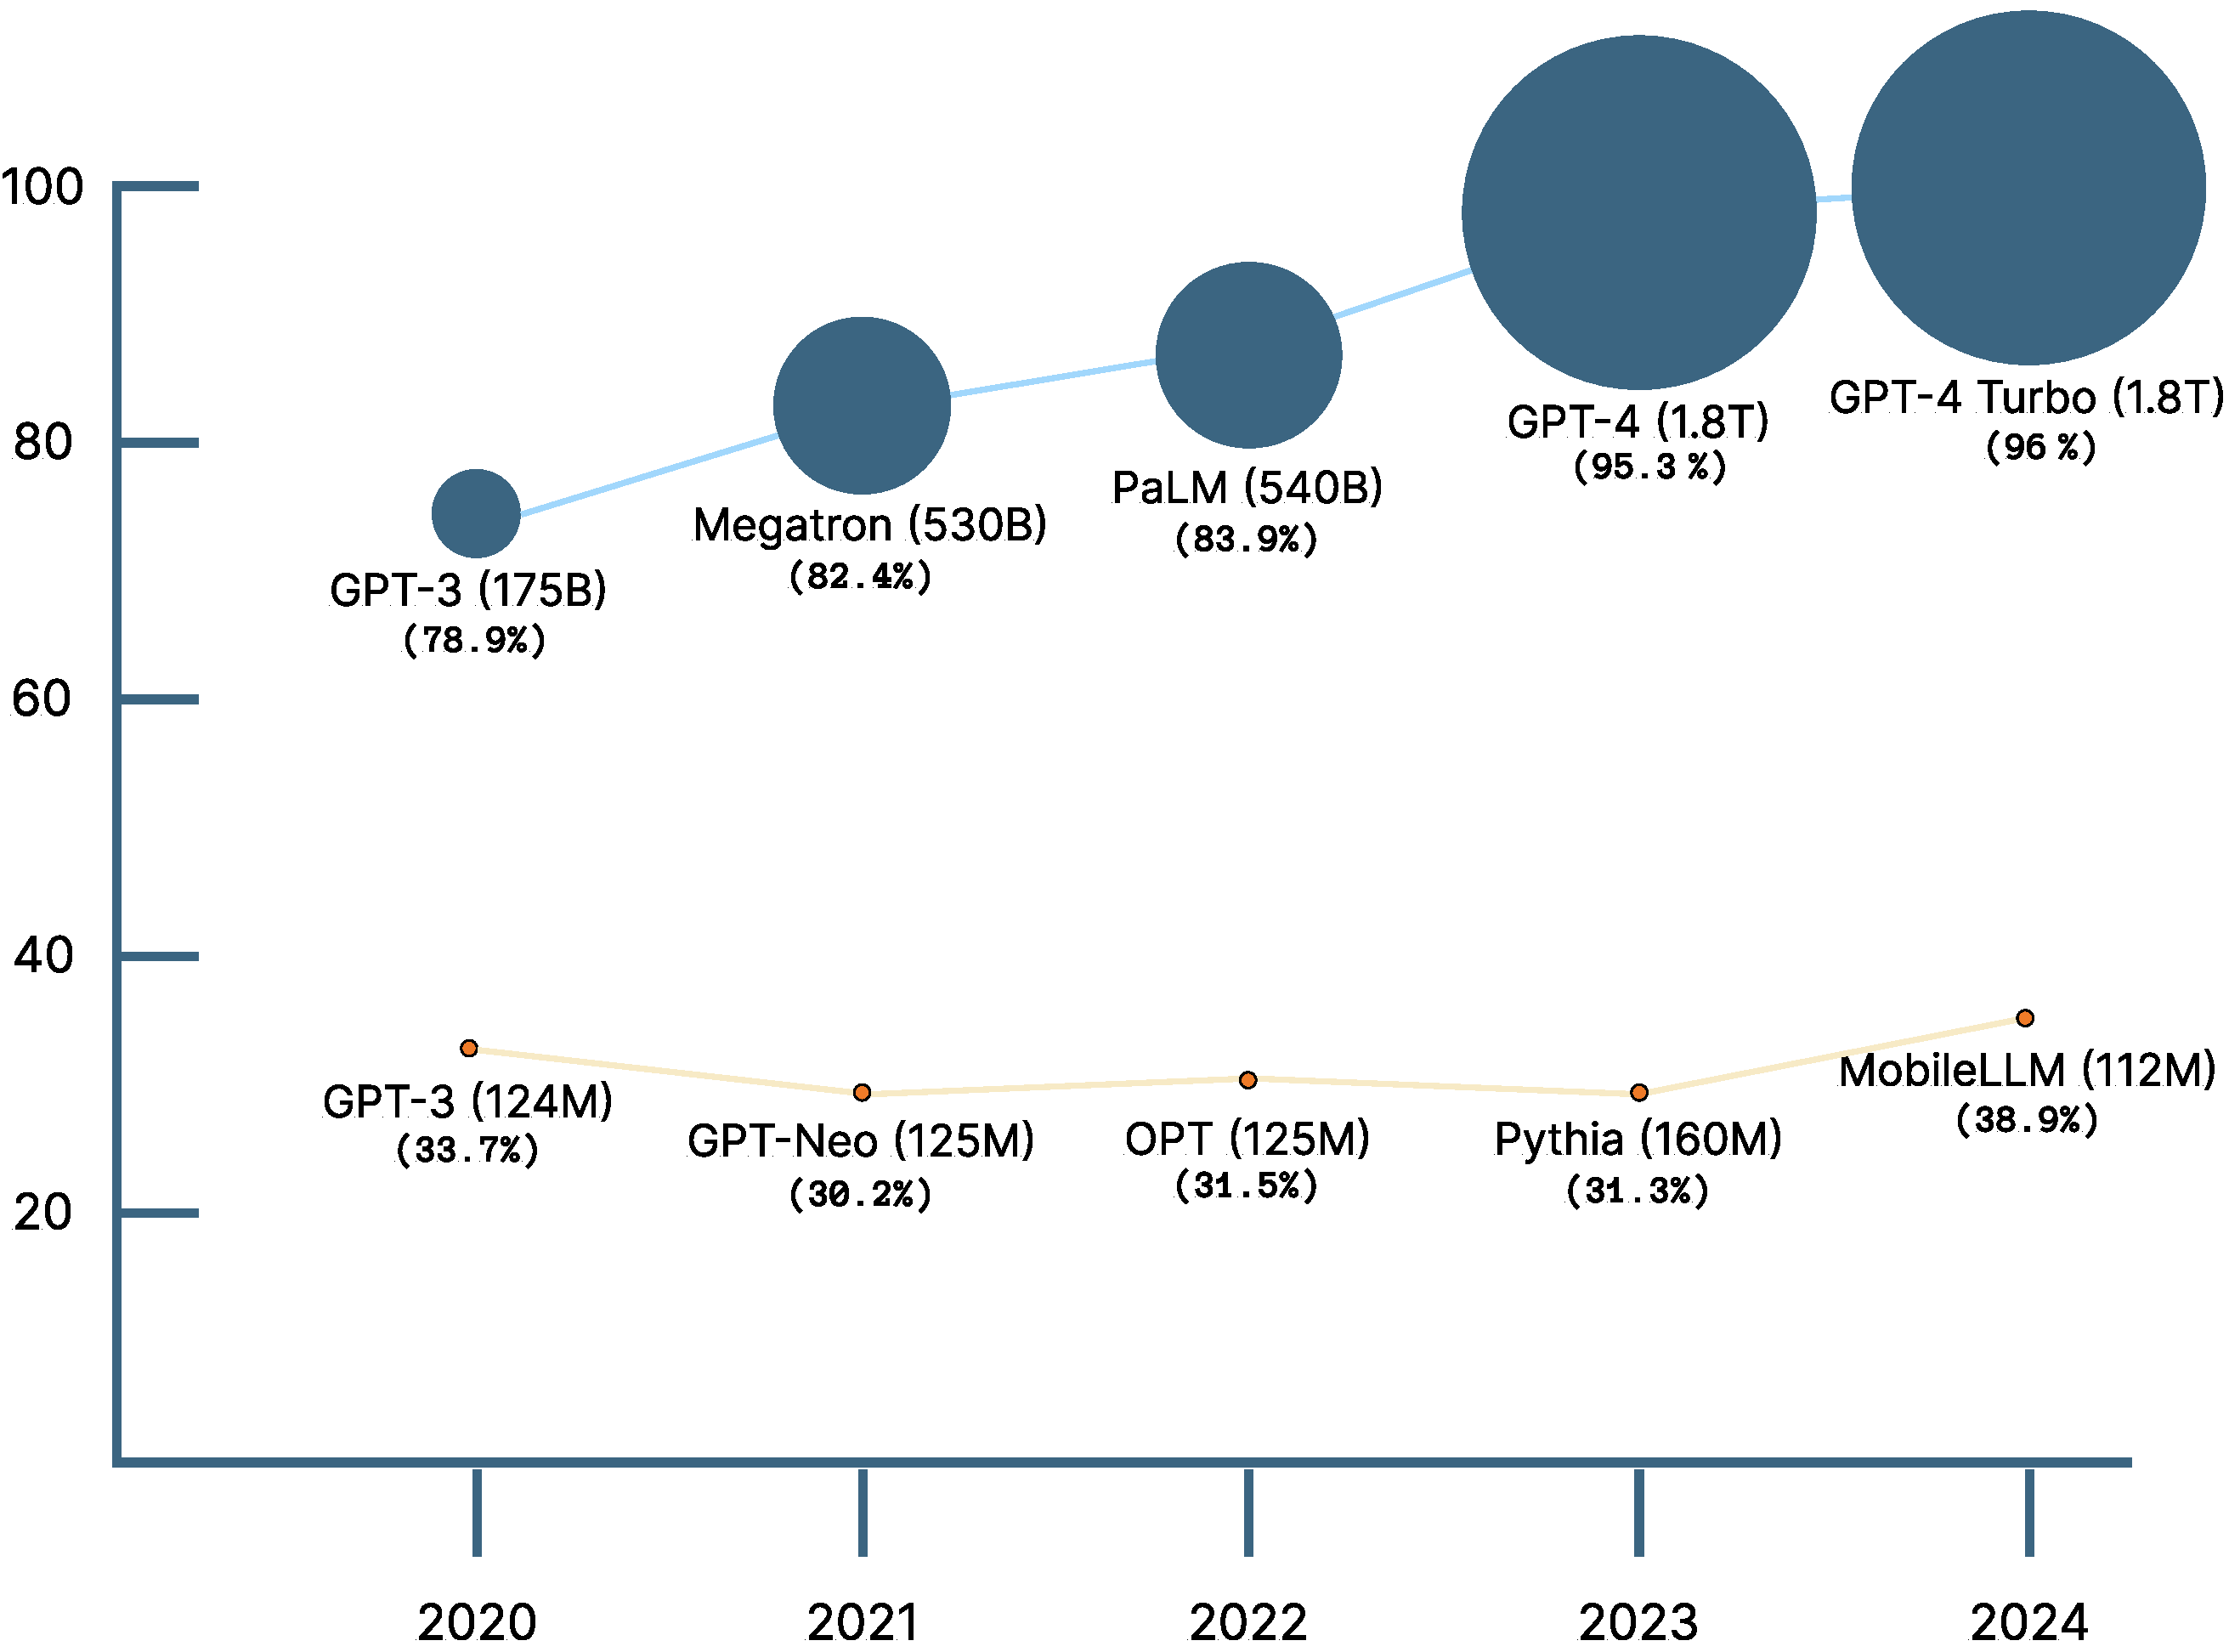
\includegraphics[width=0.8\textwidth]{chapters/introduction/figures/lm_performance_comparison.pdf}
    \caption{Performance of small and large language models on the HellaSwag dataset over time. The plot reveals a striking divergence: while \textbf{\textcolor[HTML]{37718E}{large}} models show consistent improvement, \textbf{\textcolor[HTML]{FF7F11}{small}} models have plateaued despite advances in training techniques.}
    \label{fig:model_size_vs_performance}
\end{figure}

This insight extends beyond academic interest. While frontier models dominate public and industrial attention, small language models remain vital for several reasons. %They are not only essential for deployment in resource-constrained environments—such as mobile devices and edge computing—but also play a critical role in enabling transparency, reducing costs, and improving accessibility across a wider range of applications.

\section*{Why Do Small Models Matter?}

% We should also probably define what we mean by small models.

The rapid scaling of language models has brought about remarkable capabilities, but it has also surfaced a host of challenges and risks \citep{bommasani2021foundation}. Small language models, which are compact, efficient, and accessible, offer a promising counterbalance.

\paragraph{Large models introduce significant societal risks.} As enumerated by the Stanford Center for Research on Foundation Models \citet{bommasani2021foundation}, these include the potential for generating disinformation and misinformation at scale, amplifying biases and discrimination present in training data, and memorizing and regurgitating sensitive or copyrighted content. The sheer scale of these models also raises concerns about labor displacement, environmental impact, and the creation of single points of failure, as a widely deployed model that is compromised could have cascading negative effects across all downstream applications. Notably, the authors highlight that the risks associated with large models are not just technical but also social, as they can entrench power in the hands of a few organizations and make it harder to adapt models to specific, local needs.

\paragraph{Large models pose serious environmental sustainability challenges.} As a result, researchers have increasingly emphasized energy efficiency as a core evaluation metric, on par with traditional measures like accuracy \citep{schwartz2020greenai}. Studies have quantified the financial and carbon costs of training state-of-the-art NLP systems, revealing orders-of-magnitude differences between large and small models \citep{strubell2019energy}. For example, a modest increase in translation accuracy can result in a dramatic rise in compute cost. Tools like the ML Emissions Calculator \citep{lacoste2019quantifying} and systematic reviews of emissions factors \citep{luccioni2023counting} have made it clear that model size, hardware, and training recipes all play a role in determining the environmental footprint of machine learning. Transformer-based models, in particular, are among the most energy-intensive, especially when techniques like neural architecture search are used. Benchmarks such as HULK \citep{zhou2021hulk} have compared pretrained models' energy efficiency, showing that smaller models are far more efficient in both time and cost. Furthermore, the location where models are trained can significantly affect emissions, and sparsely activated models can be much more energy-efficient than their dense counterparts \citep{patterson2021carbon}. The overall trend is clear: smaller models are more sustainable, and their adoption is crucial for reducing AI's environmental impact.
%TODO: Last two sentences are a bit of a non sequitur.

\paragraph{Data privacy and memorization risks are heightened in large models.} Research has shown that neural networks, especially large ones, can memorize and regurgitate rare or sensitive training data \citep{feldman2020neural, carlini2019secret}. Follow-up studies have demonstrated that memorization increases with model size and data duplication, and have introduced methods to extract such memorized content from models without access to the original training set \citep{carlini2021extracting, carlini2022quantifying}. Comprehensive surveys have categorized the security and privacy risks of large language models, including inference-time leakage, adversarial vulnerabilities, and systemic risks from centralization \citep{yao2024privacysurvey}. Larger models are more likely to leak personally identifiable information, especially when trained on duplicated or low-diversity data \citep{huang2022large, neel2023privacy}. Mitigation strategies such as differential privacy \citep{dwork2006calibrating} and federated learning \citep{mcmahan2017communication} have been proposed, but these often come with trade-offs in model utility. Scaling laws for memorization further confirm that as models grow, so does their propensity to memorize and leak sensitive information \citep{lu2024scaling, biderman2023emergent, kiyomaru2024comprehensive}. In contrast, smaller models, with less capacity to memorize, offer a more privacy-preserving alternative—especially when combined with privacy-focused training techniques.

\paragraph{Small models are uniquely suited for on-device and edge deployment.} Efficient inference with limited memory is essential for running language models on consumer hardware, and recent work has shown that even models with billions of parameters can be optimized for such use cases \citep{alizadeh2024llm}. Sub-billion parameter models are particularly important for energy-efficient, on-device applications, as demonstrated by \citet{liu2024mobilellm}. Earlier advances in mobile-friendly architectures, such as MobileNets \citep{howard2017mobilenets} and EfficientFormer \citep{li2022efficientformer}, laid the groundwork for efficient models in both vision and language domains. The importance of energy-proportional memory for datacenter and mobile applications has also been highlighted \citep{malladi2012towards}. These advances make it possible to run language models in privacy-sensitive, resource-constrained, or offline settings, broadening the reach and utility of AI.

\paragraph{Interpretability and scientific understanding are further reasons to prioritize small models.} The internal mechanisms of transformers and other neural architectures are more tractable in smaller models, making them better testbeds for developing scientific understanding \citep{elhage2021mathematical, elhage2022toy, bircken2023monosemanticity, anthropic2023components}. Tools such as influence functions are easier to apply at small scale, and the "manifold hypothesis" suggests that smaller models are ideal for probing the structure of neural representations \citep{olah2014manifolds}. Progress in understanding larger models often begins with insights gained from studying their smaller counterparts.

\paragraph{Finally, the democratization and accessibility of language technology depend on the availability of small, open models.} The cost of training and deploying large models is rising rapidly, with the financial and hardware requirements putting them out of reach for most organizations and individuals \citep{cottier2024rising, sharir2020cost}. Minimal, well-documented implementations like nanoGPT \citep{karpathy2023nanogpt} and Pico \citep{diehlmartinez2025pico} make language modeling accessible to a broader community, supporting education, experimentation, and innovation. By lowering the barrier to entry, small models enable more researchers, organizations, and communities to participate in the development and application of language technologies.

% In summary, small language models matter because they are more sustainable, privacy-preserving, interpretable, and accessible. They offer a practical and ethical path forward for language technology, especially as the risks and costs of large-scale models continue to mount.

\section*{Research Objectives}

This thesis aims to explore how small language models can be trained more efficiently and effectively, emphasizing principled approaches over brute-force scaling. The work is structured around two central research objectives:

\begin{quote}
    \textbf{Research Question 1: Can insights from human language acquisition be leveraged to develop more principled and effective training paradigms for small language models?}
\end{quote}

Despite recent advances in architecture design and compression techniques, small models continue to lag behind their larger counterparts. Yet they are critical for real-world deployment due to their efficiency, interpretability, and accessibility.

A persistent challenge in this area is that many of the methods proposed to improve small models, ranging from ad hoc architectural tweaks to various forms of regularization or data augmentation, often lack a strong scientific foundation. Progress is frequently incremental and difficult to interpret; new techniques sometimes offer only marginal gains or fail to generalize beyond specific benchmarks. Without a principled framework or guiding thesis, it becomes challenging to systematically understand what works, why it works, and how to build on prior results in a cumulative way.

One promising guiding thesis is to look to human language acquisition for inspiration. While today's large language models are trained on trillions of tokens, a typical 13-year-old human has been exposed to only around 100 million words. This dramatic discrepancy highlights a key inefficiency in current training paradigms and suggests an opportunity: do strategies that work well for the human brain also confer advantages in artificial models? And can cognitive science offer a roadmap toward more efficient, adaptable, and robust language modeling?

By grounding small model training in insights from human cognition, this thesis seeks to move beyond ad hoc heuristics and toward a more principled, theory-driven foundation. Rather than treating efficiency as an afterthought, the goal is to understand how cognitive strategies, such as curriculum learning, inductive biases, and compositional generalization, might translate into practical improvements in model design and training. In doing so, this work aims to bridge the gap between machine learning and cognitive science, offering not only empirical results but also conceptual tools for building small language models that are both efficient and robust.

To complement this exploration of training strategies, the second research objective focuses on understanding the learning dynamics of small models more deeply and rigorously.

\begin{quote}
    \textbf{Research Question 2: How can we more quantitatively understand how small models learn and what makes them different from large models?}
\end{quote}

Improving training efficiency is only part of the broader challenge. Equally important is developing a deeper understanding of the underlying learning dynamics that drive how language models learn: How can we quantitaively study the learning process of language models? And how can we characterize the differences in learning between small and large models in a systematic, interpretable way? These questions demand not just better engineering, but a more scientific, principle-driven approach to model understanding.

In recent years, efforts to improve small language models have often relied on empirical heuristics, ranging from architecture tweaks to training tricks, that offer marginal gains but lack deeper explanatory power. This trial-and-error mindset can obscure the mechanisms behind success and makes it difficult to generalize progress across tasks, model sizes, or domains. Small models, by contrast, offer an opportunity to observe the learning process more transparently. Their smaller size makes them easier to study, as they are less complex, faster to train, and more accessible for detailed analysis.

To make progress, we must go beyond outcome-based benchmarks and focus on the learning process itself: how knowledge is acquired, how model capacity is structured and used, and how different factors shape convergence dynamics. Small models provide a unique lens for this investigation not only because they are easier to analyze, but because their behavior often reveals the underlying structure of learning in ways large models conceal.

This research objective, therefore, is grounded in the belief that meaningful progress in model development must be built on a deeper understanding of the learning process itself. By focusing on measurable, interpretable properties of training, such as model convergence dynamics and representational capacity, we can begin to articulate a more cumulative and principled science of language model development.

\section*{Thesis Overview}

This thesis is organized into two parts, reflecting the two research threads:

\subsection*{Part I: Cognitive Insights for Efficient Training (Chapters 2–4)}

\begin{itemize}

    \item \textbf{Chapter 2:} \emph{The Evolution of Language Modeling: Foundations, Scale, and Efficiency} offers a comprehensive overview of the development of language modeling, tracing its trajectory from early statistical approaches to contemporary neural methods. The chapter begins with foundational concepts, including n-gram models, and progresses through key milestones such as neural language models, word embeddings, and the advent of attention mechanisms. It analyzes how large-scale language models have transformed the field, introducing emergent capabilities and shifting the research landscape. At the same time, it highlights the increasing relevance of smaller, more efficient models. The chapter reviews major strategies for enhancing the efficiency of small models, encompassing architectural innovations, optimization techniques, and data calibration methods. It concludes by drawing connections between machine learning and cognitive science, considering how insights from human language acquisition can inform more principled model development, especially in resource-constrained environments.


    \item \textbf{Chapter 3:} \emph{Language Learning with Limited Data: Insights from Human Development for Curriculum Design}  
    explores a systematic investigation of curriculum learning strategies inspired by human language acquisition, focusing on their application to small language models. The work is motivated by the striking efficiency of human language learning compared to current language models, raising the question: can insights from human development inform more efficient training paradigms for artificial systems?

    The chapter introduces \textbf{\texttt{CLIMB}} (Curriculum Learning for Infant-inspired Model Building), a framework that operationalizes three key aspects of human language acquisition into the framework of curriculum learning: a vocabulary curriculum that gradually expands the model's lexicon, mirroring infant vocabulary development; a data curriculum that orders training inputs by linguistic complexity; and an objective curriculum that transitions from coarse word-class prediction to fine-grained masked language modeling.

    Using the BabyLM Challenge's strict 10-million-word training cap as a testbed, the work develops a meticulously optimized "vanilla" BabyBERTa baseline that advances the state-of-the-art for small models through careful tuning of architecture, vocabulary, and preprocessing. The empirical results reveal that while individual curricula don't consistently outperform this baseline, they offer selective advantages on specific linguistic tasks, particularly in syntactic evaluation.

    \item \textbf{Chapter 4:} \emph{Learning Words Like Humans Do: Syntactic Smoothing for Language Model Training}  
    explores how language models can learn word representations more like humans do, by leveraging syntactic structure to improve the representation of infrequent tokens. This work addresses a fundamental challenge in language modeling: while humans excel at learning new words through their innate ability to leverage linguistic structure, current language models often struggle to effectively represent tokens that appear rarely in their training data. This inefficiency stems from the maximum likelihood training objective, which disproportionately optimizes frequent tokens while leaving infrequent ones with insufficient learning signals. In contrast to human language acquisition, where syntactic knowledge helps bootstrap understanding of new words, language models are forced to learn primarily through frequency statistics, pushing infrequent tokens into a narrow manifold of the representational space. This leads to both frequency bias and anisotropy in the model's linguistic capabilities. Inspired by how humans leverage syntactic knowledge to learn new words efficiently, we introduce \textbf{\texttt{Syntactic Smoothing}}, a novel technique that improves token representations by incorporating linguistic structure into the learning process. By using part-of-speech distributions as a proxy for syntactic similarity—mirroring how humans use grammatical knowledge to understand new words—our method enables infrequent tokens to benefit from the learning signals of syntactically similar tokens. This approach not only reduces frequency bias and anisotropy but also demonstrates how insights from human language acquisition can lead to more principled and effective training paradigms for language models.

\end{itemize}

\subsection*{Part II: An Analytical Lens on Learning Dynamics (Chapters 5-7)}

\begin{itemize}
    \item \textbf{Chapter 5:} \emph{Model Analysis Background} provides a background on the methods used to analyze language models, including activation patterns, parameter rank, and convergence behavior.

    \item \textbf{Chapter 6:} \emph{Tending Towards Stability: Convergence Challenges in Small Language Models}  
    investigates why small models often saturate during training. Using the Pythia model suite, it analyzes activation patterns, parameter rank, and convergence behavior.

    \item \textbf{Chapter 7:} \emph{Pico: A Lightweight Framework for Studying Language Model Learning Dynamics}  
    presents Pico, a modular framework for transparent training and in-depth analysis of learning dynamics, enabling reproducible experiments with small models.
\end{itemize}

\section*{Contributions}

This work contributes to the field by:

\begin{enumerate}
    \item Exploring an in-depth analysis of the curriculum learning paradigm from a cognitive perspective.

    \item Introducing novel methods—such as syntactic smoothing and structured curricula—for improving small model generalization.

    \item Developing analysis tools to diagnose and analyze inefficiencies in model training.

    \item Construction of an open-source framework for studying language model learning dynamics that can inform better training methods.
\end{enumerate}

Together, these contributions aim to support a more \textbf{accessible, efficient, and sustainable future} for language modeling—particularly for researchers and developers working under real-world constraints.

\section*{Publications}

The content of this thesis is comprised of the following published conference papers and software packages.

\begin{tcolorbox}[
    enhanced,
    colback=white,
    colframe=thesisblue,
    arc=0mm,
    boxrule=1pt,
    left=10pt,
    right=10pt,
    top=10pt,
    bottom=10pt,
    title=Published Works,
    fonttitle=\bfseries,
    coltitle=white
]
\subsection*{Thesis Publications}
The following papers and software packages form the core content of this thesis.

\begin{itemize}
    \item Richard Diehl Martinez, Zebulon Goriely, Hope McGovern, Christoper Davis, Andrew Caines, Paula Buttery, Lisa Beinborn (2023). {\color{thesisblue}\href{https://aclanthology.org/2023.conll-1.10/}{CLIMB – Curriculum Learning for Infant-inspired Model Building}}. In \emph{Proceedings of the BabyLM Challenge at the 27th Conference on Computational Natural Language Learning}, pages 138-154, Singapore. Association for Computational Linguistics.

    \item Richard Diehl Martinez, Zebulon Goriely, Andrew Caines, Paula Butery, Lisa Beinborn (2024). {\color{thesisblue}\href{https://aclanthology.org/2024.emnlp-main.486/}{Mitigating Frequency Bias and Anisotropy in Language Model Pre-Training with Syntactic Smoothing}}. In \emph{Proceedings of the 2024 Conference on Empirical Methods in Natural Language Processing}, pages 8541-8565, Miami, Florida, USA. Association for Computational Linguistics.

    \item Richard Diehl Martinez, Pietro Lesci, Paula Buttery (2024). {\color{thesisblue}\href{https://aclanthology.org/2024.findings-emnlp.246/}{Tending Towards Stability: Convergence Challenges in Small Language Models}}. In \emph{Findings of the Association for Computational Linguistics: EMNLP 2024}, pages 4253-4263, Miami, Florida, USA. Association for Computational Linguistics.

    \item Richard Diehl Martinez, David Demitri Africa, Yuval Weiss, Suchir Salhan, Ryan Daniels, Paula Buttery (2025). {\color{thesisblue}\href{https://github.com/pico-lm}{Pico: A Lightweight Framework for Studying Language Model Learning Dynamics}}. In Submission to \emph{2025 Conference on Empirical Methods in Natural Language Processing System Demonstration Track}.
\end{itemize}
\end{tcolorbox}

\newpage

\begin{tcolorbox}[
    enhanced,
    colback=white,
    colframe=thesisblue,
    arc=0mm,
    boxrule=1pt,
    left=10pt,
    right=10pt,
    top=10pt,
    bottom=10pt,
    title=Additional Works,
    fonttitle=\bfseries,
    coltitle=white
]
\subsection*{Mentored Works}
I mentored the following projects during my PhD.

\begin{itemize}
    \item David Demitri Africa, Richard Diehl Martinez, Paula Buttery (2025). {\color{thesisblue}{Examining the Performance Gap: Meta-Learning for Pretraining Small Language Models}}. In Submission to \emph{BlackBox Workshop at the 2025 Conference on Empirical Methods in Natural Language Processing}.
    \item Yuval Weiss, Richard Diehl Martinez, Andrew Caines, Paula Buttery (2025). {\color{thesisblue}{Investigating ReLoRA: Effects on the Learning Dynamics of Small Language Models}}. In Submission to \emph{BlackBox Workshop at the 2025 Conference on Empirical Methods in Natural Language Processing}.
\end{itemize}

\subsection*{Other Publications}
I also worked on the following papers during my PhD (not included in this thesis).

\begin{itemize}
    \item Cole Simmons, Richard Diehl Martinez, Dan Jurafsky (2024). {\color{thesisblue}\href{https://aclanthology.org/2024.ml4al-1.20/}{SumTablets: A Transliteration Dataset of Sumerian Tablets}}. In \emph{Proceedings of the 1st Workshop on Machine Learning for Ancient Languages}, pages 192-202, Bangkok, Thailand. Association for Computational Linguistics.
    \item Zebulon Goriely, Richard Diehl Martinez, Andrew Caines, Paula Buttery, Lisa Beinborn (2024). {\color{thesisblue}\href{https://aclanthology.org/2024.conll-babylm.4/}{From Babble to Words: Pre-Training Language Models on Continuous Streams of Phonemes}}, In \emph{Proceedings of the BabyLM Challenge at the 27th Conference on Computational Natural Language Learning}, pages 37-53, Miami, Florida, USA. Association for Computational Linguistics.
    \item Suchir Salhan, Richard Diehl Martinez, Zebulon Goriely, Paula Buttery (2024). {\color{thesisblue}\href{https://aclanthology.org/2024.conll-babylm.15/}{Less is More: Pre-Training Cross-Lingual Small-Scale Language Models with Cognitively-Plausible Curriculum Learning Strategies}}, In \emph{Proceedings of the BabyLM Challenge at the 27th Conference on Computational Natural Language Learning}, pages 174-188, Miami, Florida, USA. Association for Computational Linguistics.
    \item  Richard Diehl Martinez$^{\dagger}$, Suchir Salhan$^{\dagger}$, Zebulon Goriely, Paula Buttery (2025). {\color{thesisblue}{How Long Can a \textsc{BabyLM} Go? Investigating the Effect of Sequence Length on Small Language Model Pre-Training}}. In Submission to \emph{2025 BabyLM Workshop at the Conference on Empirical Methods in Natural Language Processing}. $^{\dagger}$Equal contribution.
\end{itemize}
\end{tcolorbox}

\chapter{Curriculum Learning for Infant-inspired Model Building: A Framework for Human-like Language Acquisition}
\label{chapter:CLIMB}

\newtcbox{\lightorangehighlight}{on line, colback=orange!10, boxrule=0.2mm, left=0.5mm, right=0.2mm, top=0.2mm, bottom=0.2mm}
\newtcbox{\darkorangehighlight}{on line, colback=orange!25, boxrule=0.2mm, left=0.5mm, right=0.2mm, top=0.2mm, bottom=0.2mm}

\newtcbox{\lightgreenhighlight}{on line, colback=green!10, boxrule=0.2mm, left=0.5mm, right=0.2mm, top=0.2mm, bottom=0.2mm}
\newtcbox{\darkgreenhighlight}{on line, colback=green!25, boxrule=0.2mm, left=0.5mm, right=0.2mm, top=0.2mm, bottom=0.2mm}
\newtcbox{\verydarkgreenhighlight}{on line, colback=green!40, boxrule=0.2mm, left=0.5mm, right=0.2mm, top=0.2mm, bottom=0.2mm}

\newtcbox{\lightpurplehighlight}{on line, colback=purple!10, boxrule=0.2mm, left=0.5mm, right=0.2mm, top=0.2mm, bottom=0.2mm}
\newtcbox{\darkpurplehighlight}{on line, colback=purple!25, boxrule=0.2mm, left=0.5mm, right=0.2mm, top=0.2mm, bottom=0.2mm}
\newtcbox{\verydarkpurplehighlight}{on line, colback=purple!40, boxrule=0.2mm, left=0.5mm, right=0.2mm, top=0.2mm, bottom=0.2mm}


While the background chapter established how human learning principles can inform language modeling, this chapter puts these ideas into practice through a concrete framework for curriculum learning. We present CLIMB (Curriculum Learning for Infant-inspired Model Building), a systematic approach to implementing developmentally plausible training protocols for language models. Our work is motivated by three key observations:

First, the current paradigm of language model training that relies on large datasets and computational resources stands in stark contrast to human language acquisition. Children acquire sophisticated language capabilities from only a few million words per year \citep{gilkerson2017mapping}, while state-of-the-art language models require trillions of tokens and extensive computational resources \citep{zhang2021need, zhao2023llmsurvey}. This discrepancy raises fundamental questions about the efficiency of current training approaches.

Second, conventional language model training differs from human learning in its structure: models operate on a predetermined static vocabulary and optimize a fixed objective on randomly shuffled data. In contrast, human language acquisition follows a carefully orchestrated progression: from babbling to simple utterances, and eventually to complex syntax and abstract meaning. This developmental trajectory suggests that structured learning protocols might enable more efficient model training.

Third, while curriculum learning has shown promise in various machine learning domains \citep{bengio2009curriculum}, its application to language modeling remains fragmented. Previous work has explored individual aspects such as vocabulary progression, data sequencing, or objective simplification but lacks a unified framework for implementing and evaluating these strategies, particularly in resource-constrained settings.

To address these challenges, we develop CLIMB within the context of the BabyLM Challenge \citep{warstadt2023babylm1}, which provides an ideal testbed for exploring cognitively plausible training protocols under strict data constraints (10 million words). Our framework systematically implements three curriculum dimensions:

\begin{itemize}
    \item \textbf{Vocabulary Curriculum:} Gradually expanding the model's lexicon, mirroring how children build their vocabulary from concrete nouns and verbs to more abstract terms.
    \item \textbf{Data Curriculum:} Structuring training data to progress from simpler to more complex linguistic structures, following the developmental trajectory observed in child language acquisition.
    \item \textbf{Objective Curriculum:} Evolving learning objectives from broad linguistic categories to specific token prediction, similar to how children first grasp word classes before mastering precise lexical distinctions.
\end{itemize}

Our work makes several key contributions:

\begin{enumerate}
    \item We establish a novel framework for categorizing and implementing curriculum learning strategies that simulate human language acquisition, providing a foundation for future research in cognitively inspired language modeling.
    
    \item Through extensive experimentation, we evaluate the effectiveness of different curriculum approaches under real-world constraints, offering concrete recommendations for when and how to apply specific curriculum strategies.
    
    \item We demonstrate that careful model and hyperparameter selection can yield strong performance even with limited data, with our vanilla models outperforming shared task baselines on grammatical knowledge (BLiMP) and approaching state-of-the-art performance on natural language understanding (SuperGLUE).
    
    \item We provide insights into the interaction between different curriculum dimensions, suggesting directions for developing more integrated approaches to curriculum learning in language modeling.
\end{enumerate}

The remainder of this chapter is organized as follows: Section 2 reviews the theoretical foundations of curriculum learning and its application to language modeling. Section 3 details our methodology, including the CLIMB framework and experimental setup. Section 4 presents our results and analysis, comparing different curriculum strategies and their combinations. Section 5 discusses the implications of our findings and directions for future work. Finally, Section 6 concludes with key insights and recommendations for implementing curriculum learning in language modeling.

\section{Methodology}

The work in this chapter is conducted within the context of the BabyLM Challenge \citep{warstadt2023babylm1}, which provides a constrained setting (10 million words) for exploring cognitively plausible training protocols. Before implementing our curriculum learning strategies, we first establish a strong baseline model and data processing pipeline. 

\subsection{Model Architecture and Training Setup}
All of our models are based on an 8-layer Transformer language model (\cref{subsec:baseline}) comparable to the BabyBERTa model \cite{huebner2021babyberta}. This architecture choice was motivated by the success of smaller models in low-resource settings, as demonstrated in the original BabyBERTa work. For all experiments, we leverage several key tools and frameworks to ensure robust and reproducible training. The Hugging Face Transformers library \cite{transformers} provides our model implementation, while Weights \& Biases \cite{wandb} enables comprehensive performance tracking and experiment monitoring. We use Hydra \cite{hydra} for experiment configuration management, allowing us to systematically explore different curriculum learning strategies. All training is conducted on a high performance computing cluster to ensure efficient model development and experimentation.

\subsection{Training Data}
\label{subsec:data}

\subsubsection{Data Source and Size}
We work exclusively with the training data provided in the \textsc{strict-small} track of the BabyLM challenge. This dataset is carefully constrained to 10 million words, compiled from 10 diverse corpora to ensure a representative sample of language use. Through our preprocessing pipeline, we reduce the initial 1,058,740 newline-delineated samples to 335,858 instances, corresponding to approximately 9.4 million words.\footnote{The word count is estimated by whitespace splitting, following the same metric used by the task organizers. When applying a tokenizer, the pre-processed dataset contains 11.7 million words (including punctuation) or 13.6 million subwords, reflecting the additional tokens introduced by subword tokenization.} This reduction in instances is primarily due to our concatenation strategy for shorter sequences, which we discuss in detail below.

\subsubsection{Data Preprocessing}
The diversity of our data sources (spanning books, subtitles, transcripts, and articles) necessitated careful curation to ensure consistency across corpora. Our preprocessing pipeline implements several key transformations. First, we standardize the text through lowercasing and punctuation normalization. We then apply regular expressions to standardize typographical conventions, ensuring consistent representation of numbers, dates, and special characters. The pipeline also removes extraneous content that could interfere with language modeling, including page numbers, bibliography entries, plain text tables, and one-word on-screen actions commonly found in subtitle data.

For transcribed speech corpora (with the exception of the British National Corpus), we implement a special concatenation strategy. Contiguous sections of five lines are combined into single data instances, addressing the challenge of relatively short sequence lengths in speech data. This approach helps maximize the effective use of our model's context window. Finally, at the point of model input, we join data segments to make full use of the available sequence length, which is set to 128 subtokens. This joining strategy is particularly important for maintaining the coherence of longer texts while staying within the model's context window constraints.

\subsubsection{Part-of-Speech Tagging}

While our preprocessing pipeline ensures consistent text formatting, we also need to capture linguistic structure to support our curriculum learning experiments. In particular, our vocabulary and objective curricula (Sections \cref{subsec:vocab-cl} and \cref{subsec:objective-cl}) rely on syntactic information to guide the learning process. However, the \textsc{strict-small} track's prohibition on external resources presented a unique challenge for implementing POS tagging, as we could not use supervised taggers.

\begin{wrapfigure}{r}{0.45\textwidth}
    \centering
    \small
    \begin{tabular}{lrrr}
    \toprule
    POS Tag & Precision & Recall & F1 \\
    \midrule
    NOUN & 0.786 & 0.790 & 0.788 \\
    DET & 0.820 & 0.772 & 0.795 \\
    CONJ & 0.969 & 0.821 & 0.895 \\
    NUM & 0.592 & 0.799 & 0.681 \\
    PRON & 0.592 & 0.962 & 0.733 \\   
    VERB & 0.816 & 0.823 & 0.819 \\
    PRT & 0.501 & 0.701 & 0.584 \\
    ADJ & 0.673 & 0.554 & 0.608 \\
    ADP & 0.842 & 0.888 & 0.864 \\
    PUNC & 0.944 & 0.960 & 0.952 \\
    \bottomrule
    \end{tabular}
    \caption{\label{tbl:unsupervised-pos-performance} Performance metrics of our unsupervised POS tagger compared to NLTK's supervised system.}
\end{wrapfigure}

To address this, we developed an unsupervised approach using the \texttt{anchor-features} algorithm \cite{stratos2016unsupervisedpos}, which identifies "anchor words" strongly associated with specific grammatical categories and uses these to learn a hidden Markov model (HMM). We ran this algorithm on the training dataset, and generated 30 clusters of features that each capture some latent syntactic information. We then manually mapped each cluster to a universal POS tag \cite{petrov2012universalpos}, with several clusters often mapping to the same grammatical category. Notably, our clustering approach failed to identify distinct groups for adverbs (ADV) and unknown tokens (X).

When evaluated against NLTK's supervised system \cite{bird2009natural}, our tagger showed strong performance on punctuation (F1: 0.952) and conjunctions (F1: 0.895), likely due to their consistent usage patterns. However, it struggled more with particles (F1: 0.584) and adjectives (F1: 0.608), which may have more variable usage patterns or semantic dependencies. These variations highlight the challenges of unsupervised grammatical category learning in low-resource settings.

\subsubsection{Data Availability and Observations}
To promote reproducibility and further research in this area, we provide our cleaned and tagged versions of the 10M word dataset on Hugging Face, along with the complete preprocessing scripts.\footnote{\url{https://huggingface.co/cambridge-climb}} This includes all the transformations described above, as well as the POS tagging pipeline. Interestingly, our experiments revealed that models trained on the raw, unprocessed data often outperformed those trained on our carefully preprocessed version. This counterintuitive finding, which we discuss in detail in \cref{sec:discussion}, suggests that the linguistic "noise" in raw data may actually provide valuable learning signals for language models, particularly in low-resource settings.

\subsection{Vanilla Models}
\label{subsec:baseline}

\begin{table*}
\centering
\small
\setlength{\tabcolsep}{4pt}  % Reduce column spacing
\begin{tabular}{l | rrrrr | rrrr}
\toprule
Model  & L & H & Hidden & Int. & Vocab & Steps & BLiMP & BLiMP. Supp & Perplexity \\
\midrule
Small  & 8 & 8 & 256 & 2,048   & 8,192   & 250K      & 75.43      & 61.14       & 9.46    \\
Medium & 10 & 10 & 500 & 2,000 & 8,192  & 156K      & 76.45      & 63.28        & 9.05  \\
Large  & 12 & 12 & 768 & 3,072 & 8,192   & 94K      & 75.80      & 60.83      & 9.34 \\[2mm]
\hline \\
Small  & 8 & 8 & 256 & 2,048   & 16,384  & 250K      & 76.16      & 60.85       & 13.80    \\
Medium & 10 & 10 & 500 & 2,000  & 16,384 & 94K      & 76.09      & 60.03        & 13.80     \\
Large  & 12 & 12 & 768 & 3,072 & 16,384  & 62K      & 75.08      & 63.45      & 14.22     \\
\bottomrule
\end{tabular}
\caption{\label{tbl:baseline-size-comparison} Our vanilla BabyBERTa-style models evaluated on original BLiMP and the BLiMP-like tasks prepared for BabyLM (BLiMP.Supp). Models are grouped by their vocabulary sizes. L denotes the number of Transformer layers and H the number of attention heads per layer. The Hidden dimension (Hidden) represents the size of token representations at each layer, while the Intermediate dimension (Int.) indicates the expanded dimension size in the feed-forward network (typically 4x the hidden dimension).}
\end{table*}

We investigate three different sizes of a vanilla Pre-Layer Norm RoBERTa model \cite{liu2019roberta} based on the BabyBERTa model \cite{huebner2021babyberta}: `small', `medium', and `large' -- \cref{tbl:baseline-size-comparison} lists the model configurations and presents the results for the different model sizes evaluated by perplexity, on BLiMP \cite{warstadt2020blimp} and on the supplementary BLiMP-like tasks issued by the BabyLM organizers (`Blimp.Supp'). We found the medium model with a small vocabulary size performed the best overall; however, the small model achieved similar results, and so to save on compute and keep to the restrained intentions of the \textsc{strict-small} track, we used the small model in our curriculum learning experiments.

\begin{wrapfigure}{r}{0.45\textwidth}
    \centering
    \small
    \begin{tabular}{lc}
    \toprule
         Parameter& Value\\
    \midrule
         Layer Norm EPS& 1e-5 \\
         Tie Word Embeddings & False \\
         Learning Rate & 0.001 \\
         Optimizer & AdamW \\
         Scheduler Type & Linear\\
         Max Steps & 400,000 \\
         Warm-up Steps & 100,000\\
         Per Device Batch Size & 32 \\
    \bottomrule
    \end{tabular}
    \caption{Hyperparameter settings which are constant across our vanilla models described in \cref{subsec:baseline}.}
    \label{tbl:baseline_hyperparams}
\end{wrapfigure}

We use Byte Pair Encoding (BPE) tokenization \cite{gage1994bpe} with a vocabulary of 8,192 because it yields better overall performance compared to a larger vocabulary of 16,384. The tokenizers we use in our experiments were trained on the cleaned data that we processed using the steps outlined in \ref{subsec:data}. In pilot experiments, we did not observe the benefits reported by \citet{huebner2021babyberta} from removing the unmasking procedure that is a standard component of the MLM objective \cite{devlin2019bert}, and therefore did not investigate this option further. In \cref{tbl:baseline_hyperparams} we report all of the hypereparemeters we use throughout our experiemnts.

All of the curriculum learning methods in the following sections were applied on top of our small vanilla BabyBERTa-style baseline -- to isolate the effect of the curriculum-learning training process, we fixed the architecture of the model and the model hyper-parameters. We use an AdamW optimizer with linear scheduling \cite{loshchilov2019decoupled}.

\section{A Three-Dimensional Framework for Curriculum Learning}
Curriculum learning \cite{bengio2009curriculum} is a machine-learning paradigm which optimizes a model's performance by gradually increasing the difficulty of training over time according to a set schedule (a `curriculum') -- based on the idea that learning should proceed from easy to hard, inspired by the way that humans learn \cite{elman1993learning}.
Within the context of curriculum learning, one of the central questions is how to define and manipulate the difficulty of the learning process over the course of training. In a recent survey, \citet{soviany2022curriculum} decompose this challenge into two main sub-problems: determining a sorting mechanism to assess the difficulty of instances and developing a pacing function for increasing difficulty over time. 

\begin{table*}[H]
    \centering
    \small
    \begin{tabular}{lll}
    \toprule
    \textbf{Curriculum Type} & \textbf{Parameter} &\textbf{Variants} \\
    \midrule
     \multirow{2}{*}{Vocabulary} & Selection & frequency, word class, mixed \\
     & Pacing & linear, logarithmic \\
     \midrule
     \multirow{3}{*}{Data} & Difficulty & source, unigram perplexity, self-perplexity \\
     & Pacing & linear, logarithmic \\
     & Initial Perplexity & unigram, random \\
      \midrule
     \multirow{2}{*}{Objective} & Tasks & noun-verb prediction, POS prediction, MLM\\
     & Learning Setup & sequential, multitask \\
    \bottomrule
    \end{tabular}
    \caption{\label{tbl:configurations} Curriculum learning experiments overview}
\end{table*}

\subsection{Defining Curricula across Three Dimensions}
Previous work in curriculum learning typically focuses on difficulty from a data-centric perspective, however, we note that difficulty can arise from (at least) three major elements of training a neural model: the input representation, the data sampling, and the training process. We explore curriculum learning strategies across three distinct dimensions: the vocabulary, the order of training data, and the objective function.

\subsection{Vocabulary Curriculum}
\label{subsec:vocab-cl}

We propose a novel \textbf{vocabulary curriculum} that gradually expands the model's lexicon during training, inspired by how children build their vocabulary. While large language models typically begin training with a full, fixed vocabulary, children acquire language through a more progressive process, starting with a small vocabulary that expands rapidly at a rate of eight to ten words per day \cite{weizman2001lexical}. Moreover, children prioritize learning certain word classes before others, typically mastering verbs and nouns before progressing to more abstract parts of speech \cite{bergelson2015early}.

To simulate this developmental trajectory, we implement a curriculum that begins with a limited vocabulary (10\% of tokens) and gradually expands it over the course of training. During the initial stages, tokens not included in the active vocabulary are mapped to an unknown token (\textsc{UNK}) representation. The curriculum regime spans from 25,000 to 350,000 training steps, after which all vocabulary tokens become available for the final 50,000 steps of training.

We explore three strategies for selecting which tokens to include at each stage of the curriculum:

\begin{enumerate}
    \item \lightgreenhighlight{\textbf{Frequency-based selection} (Freq)} Tokens are chosen based on their frequency in the corpus, approximated using the BPE tokenizer's ID assignments (lower IDs correspond to more frequent tokens).
    
    \item \darkgreenhighlight{\textbf{Word class-based selection} (POS)} Tokens are selected according to their grammatical category, following a progression from lexical to functional classes as observed in child language acquisition \cite{bergelson2015early}: NOUN, VERB, ADJ, PRON, DET, ADP, NUM, CONJ, PRT, PNCT. All words within a given part-of-speech category are introduced simultaneously.
    
    \item \verydarkgreenhighlight{\textbf{Hybrid selection} (Hybrid)} We combine frequency and word class constraints by sorting words by their frequency within each part-of-speech category. This approach allows for more granular control over vocabulary expansion while maintaining the developmental progression of word classes.
\end{enumerate}

The rate at which the vocabulary expands is controlled by a pacing function. We experiment with both linear and logarithmic pacing functions, with the latter potentially better reflecting the rapid early vocabulary growth observed in children. \cref{fig:pacing_fn} illustrates how the percentage of unmasked vocabulary increases over the course of training under these different pacing regimes.

\begin{wrapfigure}{r}{0.45\textwidth}    
    \centering
    \small
    \renewcommand{\arraystretch}{1}
    \begin{tabular}{cl}
    \toprule
    \textbf{Difficulty} & \textbf{Corpora} \\
    \midrule
    1 & AO-CHILDES \\
    \midrule
    \multirow{2}{*}{2} & BNC Spoken \\
                           & Switchboard \\
    \midrule
    \multirow{2}{*}{3} & Open Subtitles \\
                           & QED \\
    \midrule
    \multirow{2}{*}{4} & CBT \\
                           & Children's Stories \\
    \midrule
    5 & Simple Wikipedia \\
    \midrule
    \multirow{2}{*}{6} & Wikipedia \\
                           & Gutenberg \\
    \bottomrule
    \end{tabular}
    \caption{\label{tbl:source_order} Difficulty levels assigned to each dataset, ordered from 1 (easiest, e.g., child-directed speech) to 6 (hardest, e.g., complex written texts).}
    \vspace{-2em} % Try -0.5em, -1em, or -2em as needed
\end{wrapfigure}

This approach represents, to our knowledge, the first systematic attempt at implementing a vocabulary curriculum in language model training, offering a more cognitively plausible alternative to the standard practice of training with a fixed, full vocabulary from the outset.

\subsection{Data Curriculum}
\label{subsec:data-cl}

We implement a \textbf{data curriculum} that structures the presentation of training instances to mirror how children learn language. Unlike conventional language model training, which typically presents randomly ordered data after minimal cleaning, our approach carefully sequences training instances based on their difficulty. This is motivated by the observation that the order of training instances can significantly impact model performance \citep{schluter2018data} and by the "Goldilocks effect" in human learning, where optimal learning occurs when stimuli are neither too easy nor too hard \cite{kidd2012goldilocks}. We explore two complementary approaches to determining instance difficulty:


\begin{enumerate}

    \item \lightpurplehighlight{\textbf{Source-based difficulty} (Source)} Following \citet{huebner2021babyberta}, we order datasets based on their source, considering spoken samples as 'easier' and written texts as 'harder'. This ordering reflects the natural progression of language acquisition, where children typically learn from spoken language before mastering written forms. We implement a six-level difficulty hierarchy (\cref{tbl:source_order}), ranging from child-directed speech (CHILDES) to complex written texts (Wikipedia, Gutenberg).

    \item \darkpurplehighlight{\textbf{Static perplexity-based difficulty} (Static PPX)} While source-based difficulty provides a useful heuristic, it fails to capture the variation in complexity within each corpus. To address this limitation, we implement a more fine-grained approach using perplexity as a model-intrinsic metric of instance difficulty. Perplexity measures how well a language model predicts a sequence of words, with lower perplexity indicating that the model finds the sequence more predictable and thus potentially easier to learn from. 

    We use perplexity as a model-intrinsic metric of instance difficulty. Perplexity measures how well a language model predicts a sequence of words, with lower perplexity indicating that the model finds the sequence more predictable and thus potentially easier to learn from. We explore two distinct approaches to perplexity-based difficulty assessment. The first approach uses a static assessment, where we employ a unigram language model to evaluate perplexity once at the start of training. This method provides a simple, computationally efficient baseline that captures basic frequency patterns in the data. The unigram model's perplexity scores remain fixed throughout training, offering a consistent difficulty ranking of instances that reflects the inherent complexity of the text based on word frequencies.

    \item \verydarkpurplehighlight{\textbf{Dynamic perplexity-based difficulty} (Dynamic PPX)} The second approach implements a dynamic assessment strategy, where we periodically re-evaluate perplexity using the current model state. We perform these reassessments every 25,000 training steps, allowing the difficulty assessment to evolve with the model's growing capabilities. This dynamic approach better reflects the "Goldilocks effect" in learning, where optimal progress occurs when instances are neither too easy nor too hard \cite{kidd2012goldilocks}. As the model learns and develops, instances that were initially challenging may become more manageable, while others may reveal hidden complexities that weren't apparent at first.

    The dynamic approach presents several unique challenges that require careful consideration. The primary challenge arises at the start of training, when the model lacks sufficient exposure to provide meaningful perplexity scores. We address this initialization challenge through two complementary strategies. First, we can use a separately trained unigram model for initial perplexity evaluation, which provides a reasonable starting point for difficulty assessment (Dynamic PPX-U). Alternatively, we can begin with random sampling for the first 25,000 steps before switching to model-based perplexity evaluation (Dynamic PPX-R).

    The periodic reassessment of perplexity every 25,000 steps creates an adaptive curriculum that evolves with the model's capabilities. This approach allows us to identify instances that have become too easy (exhibiting low perplexity) and potentially deprioritize them in the training schedule. Simultaneously, we can maintain focus on instances that remain challenging (showing high perplexity) and discover instances that have moved into the "Goldilocks zone" of optimal difficulty for the current model state.

\end{enumerate}

\subsection{Objective Curriculum}
\label{subsec:objective-cl}

We develop an \textbf{objective curriculum} that evolves the learning task from broad linguistic categories to specific token prediction, mirroring how children progress from understanding word classes to mastering precise lexical distinctions. This approach is motivated by the observation that human language learning is guided by interactions with other agents (e.g., adult caregivers, siblings) who help shape the learning process. In machine learning, these interactions are modeled through the objective function that guides the model's optimization.

The standard approach to language model training uses masked language modeling (MLM), which has proven highly successful for training Transformer networks \cite{devlin2019bert}. However, psycholinguistic research suggests that MLM may not be cognitively plausible as an approximation of child language acquisition \cite{caucheteux2023evidence}. The MLM objective presents a challenging discriminative classification task, requiring the model to predict a masked token's identity from the entire vocabulary (an $N$-way classification problem). This stands in contrast to how children learn, where they first develop sensitivity to distributional patterns and gradually learn to recognize lexical categories before mastering specific word forms \cite{alishahi2010computational, gleitman1990structural}.

To better align with this developmental trajectory, we implement a curriculum that gradually increases the specificity of the learning objective. We begin with broader linguistic categories and progressively narrow down to specific token prediction. This approach is inspired by recent work that simplifies classification tasks by reducing the number of possible classes from $N$ to $K$ (where $K << N$). Previous research has explored mapping rare words to hypernyms \cite{bai2022better} or replacing words with part-of-speech tags \cite{wang2023language} or syntactic dependency relations \cite{cui2022lert}. These approaches significantly reduce task difficulty by working with a smaller set of categories.

In our implementation, we use the unsupervised POS tagger to estimate word classes and experiment with two levels of classification granularity:
\begin{enumerate}
    \item A three-way classification distinguishing between VERB, NOUN, and OTHER categories
    \item A more detailed ten-way classification using universal POS tags
\end{enumerate}

We explore two strategies for implementing this curriculum:

\begin{enumerate}
    \item \lightorangehighlight{\textbf{Sequential learning} (Seq)} We first train the model to predict word classes, then transition to the full MLM objective. This approach mirrors the developmental progression observed in children, where they first learn to distinguish between major word classes before mastering specific lexical items.
    
    \item \darkorangehighlight{\textbf{Multi-task learning} (MT)} We train the model to simultaneously predict both word classes and specific tokens, with separate task heads and optimizers for each objective. This approach allows the model to benefit from both coarse-grained and fine-grained learning signals throughout training.
\end{enumerate}

The psycholinguistic literature remains divided on how exactly word learning progresses from memorizing specific lexical items to developing generalized representations of word classes \cite{clark2015first}. Our framework provides a flexible approach to studying this progression by enabling systematic investigation of how different objective functions affect the acquisition of linguistic knowledge. By varying the timing and combination of learning objectives, we can explore different hypotheses about the relationship between category learning and specific word acquisition in language development.

This objective curriculum represents a novel approach to making language model training more cognitively plausible while maintaining the benefits of the MLM objective. By starting with broader linguistic categories and gradually increasing specificity, we aim to create a learning trajectory that better reflects human language acquisition while potentially improving the model's ability to generalize from limited training data.

\subsection{Pacing Functions} 

\begin{wrapfigure}{l}{0.50\textwidth}
    \centering
    \includegraphics[width=0.45\textwidth]{chapters/climb/figures/pacing_fns.png}
    \caption{Illustration of the linear and logarithmic pacing functions used in our vocabulary curriculum experiments. The red dotted lines denote the curriculum regime, during which the percentage of unmasked words available to the model grows.}
    \label{fig:pacing_fn}
\end{wrapfigure}

Once a notion of difficulty is set, a pacing function is needed to govern how quickly the model will progress from training on easier examples to training on harder ones \cite{wu2021when}.

We experiment with two different pacing functions: linear and logarithmic. Linear pacing functions involve a steady and consistent advancement through the curriculum. This approach ensures a gradual increase in difficulty over time. Logarithmic pacing functions, on the other hand, emphasize early exposure to ``easier'' concepts, with diminishing increments as the model's capabilities are assumed to increase. Both pacing functions have been proposed in the broader curriculum learning literature \citep{bai2022better, li2021curriculum, wu2021when}. In \cref{fig:pacing_fn} we illustrate the two pacing functions for the vocabulary curriculum.

\begin{figure}[htbp]
    \centering
    \includegraphics[width=0.9\textwidth]{chapters/climb/figures/babylm_blimp_diffs_boxplots.png}
    \vspace{1em}  % Add some vertical space between figures
    \includegraphics[width=0.9\textwidth]{chapters/climb/figures/babylm_superglue_diffs_boxplots.png}
    \caption{Comparison of model performance across BLiMP (top) and SuperGLUE (bottom) tasks. The plots show the differences in performance between our curriculum learning models and baseline models. Types of curriculum learning are indicated in the legend and highlighted with different colors with explanations in the text.}
    \label{fig:combined-boxplots}
\end{figure}


\section{Results}

Multiple evaluation metrics are employed in BabyLM. In our work, we focus on BLiMP \cite{warstadt2020blimp} and the supplementary BLiMP-style tests provided by the shared task organizers. We also report our results on the natural language understanding benchmark, SuperGLUE \cite{wang2019superglue}, and the ambiguous subset of MSGS (the Mixed Signals Generalization Set) \cite{warstadt2020msgs}. In brief, BLiMP evaluates specific linguistic abilities, MSGS evaluates linguistic preference over surface generalisation and SuperGLUE evaluates downstream task performance. For all scores, we report the average score across all categories, rather than test instances, as provided by the BabyLM evaluation pipeline.\footnote{For instance, there are 12 categories in BLiMP but 50+ individual tests. We average over the scores given for each category, rather than the scores given for each test.} All of our curriculum learning models are small BabyBERTa-style ones using the parameters shown in \cref{tbl:baseline-size-comparison} and the cleaned training dataset of 9.4M words (reduced from the 10M word dataset for the \textsc{strict-small} track) and their results can be found in \cref{tbl:result-vocab-cl}, \cref{tbl:result-data-cl} and \cref{tbl:result-obj-cl}. 


In the tables we compare to our small BabyBERTa-style vanilla model also trained on the clean data (\cref{subsec:baseline}). \cref{fig:combined-boxplots} visualizes these comparisons for the BLiMP and SuperGLUE tasks.

Furthermore, we experimented with some combinations of different curricula to see how they would interact (\cref{tbl:result-combination-cl}). For all of our runs, we use the same set of hyper-parameters that we report in \cref{tbl:baseline_hyperparams}. 


We find notable gains for our own vanilla models over the shared-task baselines, and, while we do not identify further large improvements in our curriculum learning models, we do notice some modest gains which suggest possibilities for future research and experimentation over variables. While the differences in performance between most of our experimental conditions are small, the large number of ablations we run enables us to provide a comprehensive set of recommendations for how and when different curriculum learning strategies may offer improved performance on linguistic tasks. Below we summarize our observations over the full results tables.

\begin{table*}
    \centering
    \small
    % \setlength{\tabcolsep}{3pt}  % Reduce column spacing further
    \begin{tabular}{ll|rrrrr}
    \toprule
    Pacing & Type & PPX & BLiMP & BLiMP.S & GLUE & MSGS \\
    \midrule
    \textsuperscript{\textdagger}Linear & \lightgreenhighlight{Freq} & 9.70 & 75.09 & \textbf{66.43} & 68.71 & 68.61 \\
    Linear & \darkgreenhighlight{POS} & 10.17 & 72.06 & 63.44 & 69.50 & 66.91 \\
    Linear & \verydarkgreenhighlight{Hybrid} & 10.21 & 73.37 & 66.11 & 69.22 & 66.61 \\
    Log & \lightgreenhighlight{Freq} & 9.26 & 74.97 & 64.63 & 69.94 & 66.82 \\
    Log & \darkgreenhighlight{POS} & 9.29 & 74.12 & 62.06 & \textbf{70.66} & \textbf{70.52} \\
    Log & \verydarkgreenhighlight{Hybrid} & 9.29 & 74.74 & 63.62 & 70.29 & 66.42 \\
    \midrule
    Vanilla & & \textbf{9.21} & \textbf{75.48} & 65.34 & 70.47 & 68.30 \\
    \bottomrule
    \end{tabular}
    \caption{\label{tbl:result-vocab-cl} Results for vocabulary curriculum models (\cref{subsec:vocab-cl}). All models score above 90 in the MSGS Control tasks. \textsuperscript{\textdagger} indicates the model we submitted to BabyLM, `CLIMB-tokens'. PPX = Perplexity, BLiMP.S = BLiMP.Supp, GLUE = (Super)GLUE, MSGS = MSGS Ambig.}
\end{table*}
    
We now group our experimental results according to the three curriculum learning approaches: \textbf{vocabulary}, \textbf{data}, and \textbf{objective} curricula. While our curriculum models do not uniformly outperform the vanilla BabyBERTa-style baseline, we do observe small but consistent gains in some areas. These findings point toward useful strategies for future research on curriculum learning in low-resource language modelling.

\subsection{Vocabulary Curriculum}

\paragraph{Different representations of vocabulary difficulty work better for different tasks.}
When representing difficulty in the vocabulary curriculum experiments, token ID -- our proxy for frequency -- appears to work better than word classes (POS tags) or a combination of token ID and POS tags on the BLiMP evaluation tasks, but worse than POS tags on SuperGLUE and MSGS (\cref{tbl:result-vocab-cl}).

\paragraph{Log pacing sometimes helps for vocabulary curriculum learning, but not consistently.}
While log pacing outperforms linear pacing on BLiMP in 2 out of 3 configurations and across all SuperGLUE settings (3/3), it performs worse across the board on the BLiMP Supplement tasks (0/3). This suggests that pacing strategies for vocabulary exposure are task-sensitive. It is possible that the diverse vocabulary required by BLiMP Supplement tasks may not be well captured by our current pacing functions, indicating room for future exploration of more tailored schedules or functions inspired by non-monotonic learning trajectories.

\subsection{Data Curriculum}

\begin{table*}
    \centering
    \small
%    \setlength{\tabcolsep}{3pt}  % Reduce column spacing further
    \begin{tabular}{ll|rrrrr}
    \toprule
    Pacing & Type & PPX & BLiMP & BLiMP.S & GLUE & MSGS \\
    \midrule
    Linear & \lightpurplehighlight{Source} & 10.41 & 73.32 & 61.99 & 69.68 & 66.22 \\
    Linear & \darkpurplehighlight{Static PPX} & 12.51 & 72.45 & 61.67 & 69.10 & 66.90 \\
    Linear & \verydarkpurplehighlight{Dynamic PPX-U} & 11.88 & 72.62 & 62.57 & 69.86 & 66.64 \\
    Linear & \verydarkpurplehighlight{Dynamic PPX-R} & 10.82 & 71.88 & 63.10 & 70.37 & 67.48 \\
    Log \textsuperscript{\textdagger} & \lightpurplehighlight{Source} & \textbf{9.21} & \textbf{75.87} & 64.29 & 70.20 & \textbf{70.99} \\
    Log & \darkpurplehighlight{Static PPX} & 9.39 & 75.03 & 63.78 & 69.90 & 66.69 \\
    Log & \verydarkpurplehighlight{Dynamic PPX-U} & 9.35 & 74.83 & 64.24 & 70.09 & 66.89 \\
    Log & \verydarkpurplehighlight{Dynamic PPX-R} & \textbf{9.21} & 75.81 & 63.03 & 68.93 & 66.64 \\
    \midrule
    Vanilla & & \textbf{9.21} & 75.48 & \textbf{65.34} & \textbf{70.47} & 68.30 \\
    \bottomrule
    \end{tabular}
    \caption{\label{tbl:result-data-cl} Results for data curriculum models (\cref{subsec:data-cl}). All models score above 92 in the MSGS Control tasks. \textsuperscript{\textdagger} indicates the model we submitted to BabyLM, `CLIMB-data-split'. PPX = Perplexity, BLiMP.S = BLiMP.Supp, GLUE = (Super)GLUE, MSGS = MSGS Ambig.}
\end{table*}


\paragraph{In multi-corpora datasets, ordering by difficulty is a good first step.}
Training data requirements have grown so much in modern NLP that usually training a language model from scratch will involve multiple datasets, or multiple domains. The results of our data curriculum experiments indicate that a good first step is to put these sub-corpora into some order of intuitive difficulty, as we did (\cref{tbl:result-data-cl}). In the case of BLiMP this approach outperforms our perplexity-based data curricula, and with log pacing our vanilla model. The same is true of MSGS  (with log pacing), as well as BLiMP-supplement and SuperGLUE (though the last two do not beat our vanilla model). 
Amongst the perplexity-driven models, the picture is less positive: out of 24 tests, only one model outperforms our vanilla model (log pacing, random initialisation + model perplexity in \cref{tbl:result-data-cl}).

\paragraph{Perplexity-driven approaches for data curriculum learning underperform.}
Although perplexity-based ordering intuitively reflects learning difficulty, it proves less effective in our experiments. Across 24 different perplexity-based configurations, only one outperformed our vanilla model (log pacing, random initialization + model perplexity) \cref{fig:baseline_obj_cl_superglue}. This suggests that our perplexity estimates may not capture relevant complexity for the model at small scales, and further work is needed to refine how perplexity is computed or used.


\subsection{Objective Curriculum}
\begin{table*}
    \centering
    \small
    \begin{tabular}{l@{\hspace{-15pt}}lll|rrrrr}
    \toprule
    & \multicolumn{3}{l}{Task duration (\% of training)} & & & & \\
    Type & 3 POS & 10 POS & MLM & PPX & BLiMP & BLiMP.S & S.GLUE & MSGS \\
    \midrule
    \lightorangehighlight{Seq} & -- & 0 - 12.5 & 12.5 - 100 & 9.58  & 73.87 & 62.98      & 69.85       & 66.70    \\
    \darkorangehighlight{MT} & -- & 0 - 100 & 12.5 - 100 & 9.78   & 74.60 & 62.17     & 69.12       & 66.64    \\
    \darkorangehighlight{MT} & -- & 0 - 100 & 0 - 100    & 9.30  & \textbf{75.82} & 65.77     & \textbf{70.74}       & 66.58    \\
    \lightorangehighlight{Seq} & 0 - 6.25 & 6.25 - 12.5 & 12.5 - 100 & 9.49  & 74.03 & 63.02      & 70.71       & 66.93    \\
    \darkorangehighlight{MT} & 0 - 6.25 & 6.25 - 100  & 12.5 - 100 & 9.72  & 73.68 & 63.89     & 70.07       & 67.00    \\
    \darkorangehighlight{MT} \textsuperscript{\textdagger} & 0 - 6.25 & 6.25 - 100  & 0 - 100    &  9.30 & 74.80 & \textbf{67.55}      & 69.89       & 67.65    \\
    \darkorangehighlight{MT} & 0 - 100  & -- & 0 - 100   & 9.25  & 74.48 & 63.98     & 69.77       & 67.72    \\
    \midrule
    Vanilla Model & &  & & \textbf{9.21}  & 75.48 & 65.34 & 70.47 & \textbf{68.30} \\
    \bottomrule
    \end{tabular}
    \caption{\label{tbl:result-obj-cl} Results for objective curriculum models (\cref{subsec:objective-cl}). All models score above 94 in the MSGS Control tasks. Task duration defines when an objective function was active during training, as a percentage of the total number of training steps. \textsuperscript{\textdagger} indicates the model we submitted to BabyLM, `CLIMB-multitask'. }
\end{table*}



\paragraph{Objective curricula, especially multitask setups combining POS tagging with MLM, show clear benefits on syntactic and downstream tasks.} \cref{fig:baseline_obj_cl_blimp_supp} and \cref{fig:baseline_obj_cl_superglue} compare our small BabyBERTa-style vanilla  model to our best objective curriculum learning setting -- a multi-task trained model with sequential POS-tag prediction -- on each task in BLiMP Supplement and (Super)GLUE. We find our curriculum-learning (CL) model outperforms our vanilla model on 5/6 tasks in BLiMP Supplement. While on (Super)GLUE, our CL model outperforms our baseline on 4/10 tasks and obtains comparable performance on another 4/10 tasks. This results illustrate the potential to further explore objective-curricula settings.


\begin{figure}[h]
    \centering
    \begin{subfigure}[b]{0.48\textwidth}
        \centering
        \includegraphics[width=\textwidth]{chapters/climb/figures/baseline_vs_obj_cl_blimp_supp_new.png}
        \caption{BLiMP supplementary tasks}
        \label{fig:baseline_obj_cl_blimp_supp}
    \end{subfigure}
    \hfill
    \begin{subfigure}[b]{0.48\textwidth}
        \centering
        \includegraphics[width=\textwidth]{chapters/climb/figures/baseline_vs_obj_cl_superglue.png}
        \caption{(Super)GLUE tasks}
        \label{fig:baseline_obj_cl_superglue}
    \end{subfigure}
    \caption{Comparison between our vanilla model and the best objective curriculum learning setting on different benchmark tasks.}
    \label{fig:baseline_obj_cl_comparison}
    \end{figure}

We also experimented with curriculum learning via variation in training objectives. These include sequential curricula (where objectives are swapped at fixed training stages) and multitask learning setups (where multiple objectives are trained jointly).

\paragraph{Multitask learning holds sway over sequentially swapping objective functions for now.}
In our experiments with curricula for the objective function, we compare training on simultaneous tasks -- known as multitask learning \cite{caruana1997multitask} -- with predefined sequences of objective functions which swap from one to another at set thresholds in the training process. We set up two sequential curricula: one with 2 tasks (predicting the 10 universal POS tags found in our dataset, and MLM) and the other with 3 (like the 2 task curriculum, additionally with noun/verb/other prediction). We compare these against multitasking alternatives. In general the sequential curricula are outperformed by the multitasking ones, though the 3-task sequential curriculum outperforms our BabyBERTa-style vanilla model on SuperGLUE and is second only marginally to our best-performing multitask model (\cref{tbl:result-obj-cl}). The multitask learning model with 10-class universal POS-tag prediction and MLM in place from the outset performs best on BLiMP and SuperGLUE. However, our best model on BLiMP-supplement -- a multitask one -- has an element of sequential task scheduling in that the two POS-tag prediction tasks are lined up one after the other, with a switch from 3-class to 10-class after 6.25\% of training steps. In \cref{fig:baseline_obj_cl_blimp_supp}, we visualize this result for each task in BLiMP-supplement, illustrating that our curriculum learning model improves over our vanilla model in 5/6 tasks.
Altogether, these results suggest that sequential objective function curricula do hold some potential for performance gains if further tuning of the tasks and scheduling can be carried out.

\paragraph{Sequential training has potential with tuning.}
Although multitask learning tends to dominate, some sequential objective curricula also perform well. In particular, a 3-task curriculum (noun/verb/other POS prediction $\rightarrow$ 10-class POS $\rightarrow$ MLM) yields strong performance on SuperGLUE and is only narrowly behind the multitask version. These results indicate that sequential curricula may offer further benefits if task timing and transitions are more carefully optimised.

\paragraph{Objective structure aids syntactic generalization.}
Models incorporating POS objectives---either in multitask or sequential form---often outperform vanilla models on BLiMP Supplement, which tests syntactic sensitivity. This supports the idea that structured auxiliary objectives guide the model toward syntactic generalisation, and could be explored further for syntactic evaluation tasks.


\subsection{Combined Curricula and Additional Observations}

\paragraph{In general, log pacing works at least as well as linear pacing across different curricula learning strategies.}
In our data curriculum experiments, models using the log pacing function outperform their linear counterparts in 4/4 settings on BLiMP, and 3/4 settings for BLiMP-supplement and SuperGLUE (\cref{tbl:result-data-cl}). This indicates that rapidly increasing the difficulty of training instances in the early stages brings downstream benefits on grammaticality and NLU tasks.

In our vocabulary curriculum experiments on the other hand, there is not such a clear picture. Log pacing outperforms linear in 2/3 settings on BLiMP and 3/3 on SuperGLUE, but 0/3 for BLiMP-supplement (\cref{tbl:result-vocab-cl}).
Presumably this is a reflection of the different vocabulary required by each set of evaluation tasks, which could be a matter for future investigation but also indicates that we do not yet have a clear generalizable pacing function for the vocabulary curriculum. There are of course other pacing functions to be tried.

\begin{table*}
    \centering
    \small
    \begin{tabular}{l@{\hspace{-10pt}}ll|rrrrr}
    \toprule
    Vocab \ & Data \ & Objective \ & PPX & BLiMP & BLiMP.S & S.GLUE & MSGS  \\
    \midrule
    -- & \lightpurplehighlight{Source} & \darkorangehighlight{MT} &                           9.29& 74.06 & 64.06 & 70.02 & 66.90 \\
    -- & \verydarkpurplehighlight{Dynamic PPX-R} & \darkorangehighlight{MT} &                9.44& 75.89 & 64.63 & 69.72 & 67.78 \\
    \lightgreenhighlight{Freq} & \lightpurplehighlight{Source} & -- &                     9.27& 75.89 & 64.62 & 70.24 & 67.90 \\
    \lightgreenhighlight{Freq} & \verydarkpurplehighlight{Dynamic PPX-R} & -- &        9.30& 75.88 & \textbf{65.79} & 70.42 & 66.63 \\
    \lightgreenhighlight{Freq} & \lightpurplehighlight{Source} & \darkorangehighlight{MT} &         9.22 & 74.86 & 62.82 & 70.09 & 66.68 \\
    \lightgreenhighlight{Freq} & \verydarkpurplehighlight{Dynamic PPX-R} & \darkorangehighlight{MT} & 9.46& \textbf{75.92} & 63.68 & 69.98 & \textbf{71.30} \\
    \midrule
    Vanilla Model & & & \textbf{9.21} & 75.48 & 65.34 & \textbf{70.47} & 68.30 \\
    \bottomrule
    \end{tabular}
    \caption{\label{tbl:result-combination-cl} Results for the combination curriculum models. The multitask objective curriculum refers to the 2-task 10-POS and MLM model shown in \cref{tbl:result-obj-cl}. }
\end{table*}

\paragraph{Combining all three curricula shows potential on BLiMP.}
While each individual curriculum learning experiment did not result in consistent improvements across tasks, we investigated whether combining aspects from the different curricula would, together, improve the model.
We do find that a combination of all three curricula outperforms any single curriculum model on BLiMP, but the same is not true for BLiMP-supplement and SuperGLUE (\cref{tbl:result-combination-cl}). This is another matter for future investigation, as it seems that improving each of the three curricula we investigate may lead to further gains if they are all combined.


\paragraph{In small data settings, filtering data which we intuitively think is noisy is in fact counter-productive.} Perhaps surprisingly, we find that the vanilla models trained on the raw data outperform those trained on the pre-processed data on BLiMP and MSGS. We surmise that models can learn even from linguistically non-standard datapoints.

\section{Discussion}\label{sec:discussion}

We set out to investigate a number of curriculum learning approaches to language model training, motivated by findings from the human language acquisition process and by the wish to successfully train smaller models for smaller budgets.
We first of all implemented a stronger model of our own, based on BabyBERTa \cite{huebner2021babyberta} and found that a small 8-layer vanilla model could outperform the provided BabyLM baselines on the BLiMP grammaticality tests and get close to the best RoBERTa shared-task baseline on SuperGLUE. This underlines the findings reported in the BabyBERTa paper: that with smaller datasets, it makes sense to use smaller models and a smaller vocabulary size.

The results of our curriculum learning experiments, trained with a small BabyBERTa-style vanilla model, suggest that we can further improve performance in certain linguistic tasks by careful application of a pacing function, how we represent and grow the model's vocabulary during training, select the next training instances according to their difficulty, and vary the objective function. Specifically, we find that a logarithmic pacing function works better for the data curriculum than a linear one, but the findings for the vocabulary curriculum are less clear. Other pacing functions might be tried in the future, including those that reflect acquisition theory around non-monotonic or `U-shaped' development trajectories.

It is apparent that ordering the subcorpora within a training set may be worthwhile, and that perplexity-based approaches to data selection hold potential even though we have not found a clear-cut best method for perplexity calculation as yet. As shown in other NLP work, multitask learning can be a beneficial approach, though MLM or next-word prediction remain preeminent as singular tasks used in language modeling. We find multitask learning models hard to beat in the objective curriculum, but do find good performance in our sequential settings. We believe that future work varying the timing of task switches and introducing more tasks could be worthwhile.

On a more general note, the Baby LM challenge evaluates a language model only on its final downstream performance on a set of tasks -- i.e.\ at a finite point in time. The challenge does not directly measure whether a given model is learning in a `human-like' fashion. Our contribution to the BabyLM challenge is to provide a set of curriculum learning strategies which are motivated by the language learning dynamics of infants and children. We encourage future research to study how to quantitatively evaluate whether the learning trajectory of a model parallels that of a human language learner and how similarities to human language learning results in downstream NLU performance. 


\section{Conclusions}

This chapter explored how principles from child language acquisition can guide the structure and pacing of language model training. Specifically, we implemented three curriculum learning strategies inspired by human development: gradually increasing vocabulary size (\textbf{vocabulary curriculum}), ordering training data by intuitive or model-based difficulty (\textbf{data curriculum}), and varying the specificity of the objective function over time (\textbf{objective curriculum}).

Across these experiments, we found that our BabyBERTa-style vanilla models already outperform the BabyLM baselines on BLiMP and MSGS, and perform competitively on SuperGLUE. Curriculum learning approaches offer modest but consistent gains in some areas, particularly when using log pacing functions, source-based data ordering, or multitask objectives. These results suggest that developmental structure in training can yield benefits even in resource-constrained settings.

Notably, models trained on raw, unfiltered data often outperformed those trained on cleaned data, reinforcing the idea that early exposure to linguistic variation—even if messy—may help small models generalize better, much like children learning from diverse, real-world input.

Beyond specific gains, this chapter establishes a computational framework for implementing curriculum learning strategies aligned with cognitive development. In doing so, it addresses the macro-level question posed at the start of this thesis: \textit{can language models benefit from learning more like humans do, by following a structured, developmentally inspired trajectory?} 

The next chapter builds on this foundation by shifting focus to the micro-level dynamics of representation. There, we introduce \texttt{Syntactic Smoothing}, a method motivated by how children use grammatical context to infer word meaning. While CLIMB explored how to structure the learning experience, Syntactic Smoothing investigates how to shape internal representations to support better generalization from limited exposure.


% \begin{table*}
% \centering
% \small
% \begin{tabular}{llrrrrr}
% \toprule
% Type              & Model    & PPX   & BLiMP & BLiMP.Supp & (Super)GLUE & MSGS Ambig \\
% \midrule
% Official Baseline & OPT-125m         & --    &   63.16 & 55.08 & 63.38 & 69.22 \\
%                   & RoBERTa-base      & --  &   
%                 69.84 & 50.52 & 71.42 & 70.25 \\
%                   & T5-base         & --    &   58.27 & 47.55  & 60.93 & 68.55 \\
% \midrule
% Vanilla Models    &CLIMB-base (medium)   & 9.01   & 75.66 & 66.13 & 70.75 & 67.62 \\
%                   & CLIMB-base-small & 9.21  & 75.48 & 65.34 & 70.47 & 68.30 \\
%                   & CLIMB-raw (medium)   &  8.47   & 77.97 & 66.16 & 70.63 & 69.44 \\
%                   & CLIMB-small-raw  & 8.64  & 76.42 & 64.60 & 69.46 & 70.65 \\
%                 & \emph{large-100M}      & 4.35      &   81.03 & 75.56 & 72.93 & 74.17 \\
% \midrule
% Vocab Curriculum          & CLIMB-tokens   &  9.70  & 75.09 & 66.43  & 68.71 & 68.61 \\
% Data Curriculum           & CLIMB-data-split & 9.21 & 75.87 & 64.29  & 70.20 & 70.99 \\
% Objective Curriculum      & CLIMB-multitask & 9.30 & 74.80 & 67.55  & 69.89 & 67.65 \\
% \bottomrule
% \end{tabular}
% \caption{\label{tbl:submission-comparison} Comparison between the official shared task baselines, our BabyBERTa-style vanilla models, and our submitted curriculum learning models on the main evaluation tasks: BLiMP, (Super)GLUE, and MSGS. Our *small and *medium models are defined in Section \ref{subsec:baseline}. All models are trained on pre-processed data except for those labelled with *-raw, which are trained on mostly unprocessed data (except we join the input sentences). The `large-100M' model was a larger BabyBERTa-style model trained on the 100M BabyLM training set (all others have been trained on the 10M dataset available in the \textsc{strict-small} track). }
% \end{table*}


% --- Additional Stuff ---

% \subsection{Curriculum Learning Approach}
% Our work introduces curriculum learning to three primary components of language model pre-training: vocabulary (Section \ref{subsec:vocab-cl}), data sampling approach (Section \ref{subsec:data-cl}), and objective function selection (Section \ref{subsec:objective-cl}). This multi-faceted approach is inspired by how humans learn language, where different aspects of language acquisition develop simultaneously but at different rates. For each component, we implement dynamic difficulty scaling that evolves over the course of training, simulating the progressive nature of human language learning. The specific variables and configurations for each curriculum learning experiment are detailed in Table~\ref{tbl:configurations}.

% \begin{table*}
%     \centering
%     \small
%     \begin{tabular}{llc}
%     \toprule
%          Type & Model & Training Time \\
%     \midrule
%          Vanilla Models & CLIMB-small-raw & 12h \\
%          & CLIMB-raw (medium) & 17h40m \\
%     \midrule
%          Data Curriculum & Log Source & 12h30m \\
%          & Log Random + model ppl & 17h10m \\
%          Objective Curriculum & Sequential All POS & 11h40m \\
%          & Multitask All POS & 15h30m \\
%          Vocabulary Curriculum & Linear POS & 11h50m \\
%          & Log Token ID & 12h10m \\
%     \midrule
%         Combination & Log Data Split + Log Token ID & 12h30m \\
%         & Log Random + model ppl + Log Token ID & 17h10m \\
%     \bottomrule
%     \end{tabular}
%     \caption{Compute required to train our models. We report the model with the shortest and longest runtime for each experiment type. Each model is trained for 400,000 steps with 4 A100 GPUs.}
%     \label{tbl:compute}
% \end{table*}

\chapter{Mitigating Frequency Bias and Anisotropy in Language Model Pre-Training with Syntactic Smoothing}

Humans possess a remarkable ability to quickly understand the meaning of unknown words, given contextual cues. Consider the sentence, ``the Golden Gate Bridge has been \emph{obnebulated} every morning this week, limiting visibility of the Pacific Ocean.'' For many readers, `obnebulated' is probably not a familiar term, but we are likely to infer that 1) it is almost certainly a verb because of the -ed suffix and occurrence after perfective and passive auxiliaries, and 2) its meaning relates to visibility and climatic conditions.\footnote{ `Obnebulate' is an obsolete word meaning, ``To obscure with or as with a mist; to befog'' (\emph{Oxford English Dictionary}).} The ability to integrate unknown words based on syntactic and semantic context is essential for robust language understanding and still poses a significant challenge for language models. Nevertheless, Pre-trained Transformer Language Models (PLMs) have proven tremendously capable of solving a wide array of language processing tasks \citep{touvron2023llama, chowdhery2023palm}. 

\begin{figure}[ht!]
    \centering
    \includegraphics[width=0.9\linewidth]{chapters/chapter 2/figures/blimp_bias_example.pdf}
    \caption{Illustration of the BLiMP \textbf{frequency bias} calculation used to evaluate a model's reliance on frequency statistics when making predictions. The example BLiMP values are from a baseline RoBERTa model.}
    \label{fig:blimp_bias}
    \vspace{-1em}
\end{figure}

Part of the success of PLMs can be attributed to the pre-training objective. Despite variations in architecture, the vast majority of language models are pre-trained to maximize the log-likelihood of a word, given the surrounding context \citep{devlin2019bert, brown2020gpt3, chowdhery2023palm, touvron2023llama}. As language use is characterized by a Zipfian distribution \citep{zipf1935zipflaw}, language models are exposed to frequent tokens exponentially more often than infrequent ones during pre-training. Consequently, the representations of these frequent tokens are optimized based on exponentially more learning signals than those of low-frequency tokens. It has been shown that maximum likelihood objectives lead to representation degeneration in English language models because infrequent tokens are pushed into a narrow manifold of the representational space \citep{gao2018representation}. This representation degeneration problem is linked to the broader problem of \textbf{anisotropy}: the hidden states of a language model tend to cluster together into a small cone-shaped subspace, rather than over their full representational capacity \citep{arora2016latent, ethayarajh2019contextual, gao2018representation}. As language model evaluation is based on cumulative evaluation scores that conceal how well a model processes infrequent words, the disparities in the representational space are difficult to assess.  

Conventional language modeling approaches require large model sizes to effectively capture long-tail vocabulary distributions, limiting the scalability of these methods \citep{feldman2020does,haviv2023understanding}. In this work, we propose \textbf{\texttt{Syntactic Smoothing}}: a syntactically-guided label smoothing approach to improve the representation of infrequent tokens in language models without resorting to perpetual increases of model and training data size. We smoothly distribute the backpropagation signal over syntactically similar tokens using a similarity metric based on part-of-speech (POS) tag distributions. Using this method, tokens that are seldom seen during training benefit from the more frequent updates of tokens that occur in similar syntactic functions. 
We evaluate our method using a new metric for quantifying the \textbf{frequency bias} of language models (illustrated in \cref{fig:blimp_bias}) and find that \texttt{Syntactic Smoothing} reduces both the frequency bias and the degree of anisotropy in a small English language model. We further explore the relationship between anisotropy and frequency bias and their effect on downstream performance.

\section{Related Literature}

Through maximum likelihood training, language models implicitly learn to encode token frequency statistics. This training process gives rise to a frequency bias in models that constrains their ability to generalize to infrequent tokens. In this section, we begin by reviewing literature that discusses the challenges of generalizing linguistic knowledge to infrequent tokens. We then examine recent work that links the impact of token frequency to anisotropy in the models' representational space.

\subsection{Generalization to Infrequent Tokens}

Current approaches to language modeling rely heavily on the memorization of infrequent tokens to perform well on downstream tasks \citep{feldman2020does}. Recent analytical work has shown that certain layers of transformer models implicitly store memorized long-tail data \citep{haviv2023understanding, kobayashi2023transformer}. \citet{feldman2020neural} demonstrate that models memorize atypical examples to achieve the highest accuracy on long-tailed data samples. This memorization hack, however, has only been shown to work well with over-parameterized models \citep{belkin2019reconciling}. While these studies present various metrics to evaluate memorization, these metrics do not capture how memorization impacts generalized linguistic understanding within the models. In our work, we address this gap by developing a metric that quantifies the extent of this frequency bias in relation to models' linguistic abilities.

Language use follows a Zipfian distribution, meaning that many tokens appear infrequently. Standard training objectives often require large models and noisy datasets with sufficient long-tail samples for effective generalization \citep{zheng2022memorization}. However, improving generalization without excessive scaling can be achieved by training models with inductive priors that leverage linguistic information. On the lexical level, the integration of morphological and orthographic information during representation learning has been explored to obtain more fine-grained word embeddings \citep{salle2018incorporating, vulic2017morphfitting, cotterel2015morphological, bhatia2016morphological, botha2014compositional}. To improve syntactic generalization, the objective function has been enriched with auxiliary tasks, such as predicting constituency labels \citep{wang2023language}, hypernyms \citep{bai2022better}, dependency tags \citep{cui2022lert}, and POS tags \citep{diehlmartinez2023climb}. Some approaches have also shown promising results on rare word performance by constructing token embeddings that consider a word's surface form and surrounding context \citep{schick2019attentive, schick2020rare}.

\subsection{Anisotropy in Representational Space}
While frequency bias and generalization capabilities can be observed by analyzing model behavior on input--output patterns, representational analyses indicate that these phenomena are linked to the distribution of token representations. Language models trained as likelihood maximizers have been shown to yield degenerate representations for rare tokens \citep{gao2018representation}. Throughout training, infrequent tokens are disproportionately pushed in the negative direction of most hidden states, resulting in their clustering together irrespective of their semantic or syntactic properties. This clustering behavior leads to anisotropy: rather than occupying a large region of the representational space, token representations lie along a narrow manifold \citep{gao2018representation, ethayarajh2019contextual}

\subsubsection{Defining Anisotropy}

Anisotropy is defined as the inverse of isotropy: $1-I(v(\cdot))$. A representational space is isotropic if all the vector directions are distributed uniformly, meaning no particular direction is favored over another.

\citeauthor{arora2016latent}\ and \citeauthor{mu2018all} define isotropy as:

\begin{equation}
    I(v(\cdot)) \coloneq \frac{\min_{\norm{c}=1} Z(c)}{\max_{\norm{c}=1} Z(c)}
\end{equation}
where $c$ is a unit vector and $Z(c)$ is defined as the partition function over all tokens $w$ in the vocabulary $V$ , with representations $v(w)$:
$$
    Z(c) = \sum_{w \in V} \exp(c^Tv(w))
$$
In practice, this definition of isotropy is analytically infeasible to solve. In this paper, we follow an empirical approximation proposed by \citeauthor{ethayarajh2019contextual}: 
\begin{equation}
\label{eq:empirical-isotropy}
    I(v(\cdot)) \coloneq \mathbb{E}_{i\ne j}\big(1-\cos(v(w_i), v(w_j))\big)
\end{equation}
Here, $w_i$ and $w_j$ are two tokens sampled from the vocabulary, and $\cos$ is defined as taking the cosine similarity of the two word representations for $w_i$ and $w_j$.  

Despite its prevalence, the impact of anisotropy on a model's language understanding abilities remains unclear. Some studies suggest that reducing anisotropy improves performance on non-contextual benchmarks, sentence comparison tasks, and multilingual benchmarks \citep{bis2021too, su2021whitening, rajaee2022isotropy}. Conversely, other research indicates that higher anisotropy might enhance semantic clustering tasks and that reducing anisotropy does not uniformly improve performance on common NLU tasks \citep{ait2023anisotropy, ding2022isotropy}. Furthermore, the relationship between anisotropy and maximum likelihood training has been questioned. Some researchers argue that isotropy exists in local manifolds of contextual word representations \citep{cai2020isotropy}, while others contend that anisotropy arises from the learning dynamics of the query and key attention matrices in transformer models \citep{godey2024anisotropy}.

\subsubsection{Reducing Anisotropy}

Existing methods to reduce anisotropy broadly fall into three categories. The first group of approaches transforms the hidden states of language models to remove semantically uninformative directions and to preserve the dimensions of maximal isotropy \citep{arora2016simple, mu2018all, raunak2019effective, su2021whitening,bis2021too}. This intervention style is based on the assumption that the top singular dimensions of pre-trained word representations encode frequency statistics rather than semantic or lexical information \citep{mu2018all}. The second category of methods introduces novel training objectives and regularization terms that reduce the effects of anisotropy \citep{gong2018frage, gao2018representation, wang2019improving}. This type of approach places an inductive bias on representations that push the embeddings of frequent and infrequent words to occupy a similar semantic space. The third set of approaches explores different training paradigms to directly minimize anisotropy, such as using normalizing flow models \citep{li2020sentence} or manipulating the gradients used in maximum likelihood models \citep{yu2022rare}

\vspace{1em}

While frequency bias and anisotropy are prevalent in language modeling, quantifying their effects and understanding their impact on generalization, particularly for infrequent words, remains an open area of research. Our paper introduces a novel method for improving the representation of infrequent tokens by integrating linguistic information. Moreover, we hypothesize that adjusting the learning process to better represent infrequent tokens will also reduce anisotropy, as these two phenomena are interconnected.

\section{Frequency Bias}
\label{section:freq-bias}

We investigate frequency effects using a zero-shot test of grammatical capability known as BLiMP: The Benchmark of Linguistic Minimal Pairs \cite{warstadt2020blimp}. BLiMP comprises 67 datasets (or ``subtasks''), each consisting of 1,000 pairs of grammatical and ungrammatical sentences that differ only with respect to a specific linguistic characteristic (covering syntax, morphology, and semantics). Language models are tasked with assigning a higher likelihood to the grammatical sentence. The grammatical generalization capabilities of a language model are often summarized by averaging the accuracies achieved across the 67 BLiMP tasks. While random guessing scores 0.5, state-of-the-art models have achieved scores of 0.87 when trained on large datasets, and models trained on the 10M-word BabyLM dataset have achieved scores up to 0.80 \citep{warstadt2023findings}. 

BLiMP is carefully balanced to ensure individual tokens occur equally in both sentence types. However, within a single pair, there may be an imbalance in average token frequency: For instance, the sentence
\textit{Grace's piano teachers are \textbf{known}} has a log frequency of 8.35 while its associated minimal pair \textit{Grace's piano teachers are \textbf{replied}} has a log frequency of 6.20.  We hypothesize that despite the minimal difference in BLiMP pairs, models trained in a typical manner will be biased by token frequency when determining grammatical acceptability.

Our goal is to quantify how language model performance differs between BLIMP pairs with large positive frequency differences (where the correct sentence has more frequently occurring tokens) and with large negative frequency differences (where the correct sentence has much less frequently occurring tokens). We do so in two steps.

First, for each BLIMP sentence pair, we calculate the average (natural log) frequency of the differing tokens. Frequencies of individual tokens are computed with respect to a model's training data; for instance, in the example above the token \textit{\textbf{known}} has a log frequency of 8.35 in the training data. Sentence pairs are then ranked by the relative difference in these average frequencies, where positive values indicate a higher average frequency for the acceptable sentence. These relative differences form a distribution, as shown in the middle plot of \cref{fig:blimp_bias}. 

Then, we compute the BLiMP score using pseudo log-likelihood \citep{salazar2020masked} for BLIMP pairs in the upper and lower thirds of the relative frequency difference distribution. We exclude the middle third, as these represent pairs with minimal frequency differences (see the frequency plot for details). We define a model's \textbf{frequency bias} as the difference between the two BLiMP scores. The entire process is illustrated in \cref{fig:blimp_bias}. 

In practice, we find that standard transformer language models, such as OPT-125M \citep{zhang2022opt}, RoBERTa-base \citep{liu2019roberta}, and T5-base \citep{raffel2020t5}, exhibit a frequency bias as high as 13.7\%. Our goal is to develop a model that can attain a frequency bias close to zero while attaining a high BLiMP score: that is, a model that makes determinations on the grammatical acceptability of sentences based solely on relevant linguistic aspects, rather than relying on possibly misleading statistical artifacts of the training data. 

\section{Syntactic Smoothing}

We hypothesize that transformer language models exhibit a strong frequency bias due to their maximum likelihood training objective, which limits infrequent tokens from receiving useful learning signals and thus hinders their ability to effectively encode linguistic information. To address this, we propose at each learning step to backpropagate the learning signal of a target token to all other tokens serving similar syntactic roles; this benefits infrequent tokens that appear less often in the training data.

\textbf{\texttt{Syntactic Smoothing}} implements this strategy by distributing a portion of every update signal to all syntactically similar tokens using a syntactic similarity metric (operationalized below). This results in the representation of infrequent tokens approaching the average representation of all tokens that serve a similar syntactic function; e.g., the representation of a niche word like `obnebulated' would encode its syntactic role as a verb.

Our method consists of two components; (1) a similarity metric that uses part-of-speech distributions as a coarse proxy for syntactic similarity, and (2) an adjustment to the loss function to smooth the backpropagation signal over syntactically similar tokens during pre-training. 

\subsection{Syntactic Similarity Score}\label{sec:sim}

The syntactic similarity between two tokens can be measured in multiple ways, e.g., by using surface features, dependency labels, or even the predictions of a teacher language model \citep{hinton2015distilling}. Here, we present a simple measure that acts as a coarse approximation for syntactic similarity: we consider two tokens to be similar if they have a similar distribution of part-of-speech tags in the training set.

We evaluate the syntactic similarity between tokens prior to training, as a one-off preprocessing step over the entire training set. First, we use the part-of-speech (POS) tagger from the NLTK package \citep{bird2009natural} to assign each word in the training set to one of 12 universal POS tags, based on its given context \citep{petrov2012universalpos}.\footnote{The 12 tags in the NLTK tagger are given here: \url{https://www.nltk.org/book/ch05.html\#tab-universal-tagset}. They are derived from the 17 tags in the Universal Dependencies tagset.} We then tokenize the training data into sub-word tokens and assign each token the POS tag corresponding to the word it belongs to in each instance. As words can take on a different part of speech depending on the context, we count the number of times each token in our vocabulary $V$ appears as each POS tag in the training data, producing a 12-valued vector. This results in a matrix $M \in \mathbb{R}^{|V|\times 12}$ containing the distribution over POS tags for each token. Finally, we can compute the similarity of two tokens $V_i$ and $V_j$ using the cosine similarity of their POS distributions: $$ \text{Syntactic Similarity(i, j)} = \frac{M_i^TM_j}{||M_i|| \cdot ||M_j||}$$ 


Note that while in this paper we define syntactic similarity via cosine similarity, any real-valued distance metric or divergence can be used. The similarity function does not need to be symmetric, although we note that symmetric functions provide computational advantages as only half the values need to be computed and stored. Also, note that our methodology does not depend on a specific choice of POS tagger.

We provide the POS distributions and similarity distributions for the example tokens ``blind'' and ``the'' in \cref{fig:distributions}. Notice that ``the'' occurs almost exclusively as a determiner and is not similar to many other tokens, whereas ``blind'' occurs as a noun, verb, adjective, and adverb and has a high similarity to more than half the other tokens in the vocabulary.

\begin{figure}[t]
    \centering
    \includegraphics[width=\linewidth]{chapters/chapter 2/figures/distributions.png}
    \caption{Part-of-speech distributions and similarity distributions for the subword tokens ``blind'' and ``the''. Similarities are computed as cosine-similarities against every other token in the vocabulary and sorted.}
    \label{fig:distributions}
    \vspace{-1em}
\end{figure}

\subsection{Smoothing the Backpropagation Signal}\label{section:smoothing}

Modern pre-training objectives implement likelihood maximization using a cross-entropy loss between the label of the correct word and predicted probabilities from a forward pass of the model. \texttt{Syntactic Smoothing} makes a small adjustment. Instead of a one-hot encoding, the target vector $t$ becomes a distribution across the entire vocabulary with some of the signal on the correct label $j$ and the rest of the signal distributed across all other tokens $i$ according to the syntactic similarity metric used:
\begin{equation}
\label{eq:signal-distribution}
    t_i=\left\{
  \begin{array}{@{}ll@{}}
    (1-\alpha), & \text{if}\ i=j \\
    \frac{s(i,j)}{\sum_{k=0}^{|V|}{s(i,k)}} \times \alpha & \text{otherwise}
  \end{array}\right.
\end{equation}

\noindent
where $\alpha$, the smoothing parameter, determines the proportion of the error signal reserved for the correct word and $s$ is our part-of-speech similarity metric. We experiment with different values for $\alpha$, noting that $\alpha=0$ is the standard likelihood maximization task. We also investigate the use of a pacing function that linearly decreases $\alpha$ so that at the start of training the majority of the signal is propagated to other syntactically similar tokens and by the end of training nearly all of the error signal is sent to the correct token to ensure that the model still optimizes perplexity. 

In practice, we also find it beneficial to apply a temperature scaling function to the syntactic similarity distribution. Thus, rather than using the raw syntactic similarity scores, $s(i,j)$, in \cref{eq:signal-distribution}, we use the temperature-scaled similarity scores:

$$
s'(i,j) = \frac{\exp\left(\frac{s(i,j)}{\tau}\right)}{\sum_{k=1}^{|V|} \exp\left(\frac{s(i,k)}{\tau}\right)}
$$
where $\tau$ defines the temperature which we set to $\tau=0.025$.

\subsection{Experimental Setup}
\label{subsection:experimental_setup}

Our experiments focus on smaller language models and datasets due to computational constraints and the particular challenges of generalizing to uncommon instances under resource-constrained training conditions \citep{warstadt2023findings, diehlmartinez2023climb}. 

\paragraph{Data} \label{paragraph:data} We use the dataset published as training data for the BabyLM challenge at the 2023 CoNLL workshop \citep{warstadt2023findings}. It contains roughly 10 million tokens sampled from pre-existing datasets, covering a wide range of domains including transcribed speech (both adult-directed and child-directed), movie subtitles, Wikipedia articles, and books. The dataset was constructed to be similar to the input received by children --- 56\% comes from transcribed speech and 40\% comes from sources intended for children.

\paragraph{Model} We use a small 8-layer encoder-style RoBERTa model with pre-layer normalization \cite{huebner2021babyberta}. We report the hyper-parameter settings we use throughout all experiments in \cref{tbl:appendix_hyperparams} (\cref{section:appendix-hyperparameters}) and computational requirements in \cref{section:appendix-computational-requirements}. We use a BPE tokenizer \citep{sennrich2016bpe} with a vocabulary size of 8192 as recommended in previous work \cite{diehlmartinez2023climb}. 

\paragraph{Evaluation} We evaluate the BLiMP frequency bias of our models, as defined in \cref{section:freq-bias}, on the evaluation set of BLiMP. To compute anisotropy we use the formulation defined in \cref{eq:empirical-isotropy}; We sample 1,000 pairs of random word tokens with their surrounding context from the training set, and compute the cosine similarity of their hidden representation at each of the 8 layers of the RoBERTa model. To obtain a model's final anisotropy value, we average the anisotropy scores across the 8 layers. Additionally, we finetune and evaluate each model on two downstream sentence-level tasks, COLA \citep{warstadt2019cola} and SST-2 \citep{socher2013sst}, as well as two language inference tasks, MNLI \citep{williams2018mnli} and QNLI \citep{rajpurkar2016squad, wang2018glue}.

\paragraph{Baselines}

We introduce three types of baselines: 
\begin{enumerate}
    \item \textbf{Popular open-source transformer models}: OPT-125M \citep{zhang2022opt}, RoBERTa-base \citep{liu2019roberta}, and T5-base \citep{raffel2020t5}, pre-trained from scratch on the same dataset we describe in \cref{subsection:experimental_setup}. We use the default configuration for each model resulting in a varied number of parameters.
    \item \textbf{Base Model}: The small RoBERTa model described above without \texttt{Syntactic Smoothing}.
    \item \textbf{Label Smoothing}: The base model trained with label smoothing \citep{szegedy2016rethinking}.  We train a baseline with a low-level of smoothing ($\alpha=0.2$) and a mid-level of smoothing ($\alpha=0.5$). Note that \texttt{Syntactic Smoothing} can be seen as a linguistically-guided version of the standard label smoothing approach, in which the learning signal is distributed to all tokens uniformly.
\end{enumerate}

\paragraph{Our Models} We train our models with \texttt{Syntactic Smoothing} using the same two $\alpha$ values as the label smoothing baselines to facilitate comparison. We also run variants using the linear pacing function presented in \cref{section:smoothing} which linearly decreases the smoothing from an initial value of $\alpha$ to zero across training. For these variants, we use the same two values of smoothing, as well as an additional high value of $\alpha=0.8$ giving a total of five \texttt{Syntactic Smoothing} variants.\footnote{We do not include unpaced \texttt{Syntactic Smoothing} with a high value of $\alpha$ as initial experiments found that distributing such a high proportion of the learning signal away from the correct token leads to high perplexity and poor downstream performance.}

\section{Results}
\label{sec:results}

\begin{table*}[ht!]
\centering
\small
\begin{tabular}{ll||cc|ccccc}
\toprule
\textbf{Model}  & $\alpha$ & \textbf{Bias}  & \textbf{Anisotropy} & \textbf{BLiMP} & \textbf{COLA} & \textbf{SST-2} & \textbf{MNLI} & \textbf{QNLI}  \\
\midrule
Base Model & -&9.8 & 51.3 & 71.4 & 71.4 & 82.9 & 69.6 & 79.7 \\
\midrule
\multirow{2}{*}{Label Smoothing} &Low & 5.5 & 40.2 & 73.2 & 70.7 & 84.0 & \textbf{70.1} & 80.0 \\
&Mid & 2.7  & 40.3 & 73.0 & 71.5 & 82.2 & 69.0 & 79.4 \\
\midrule
\multirow{5}{*}{\texttt{Syntactic Smoothing}}&Low  & 2.9 & 39.7 & \textbf{73.2} & 70.7 & 84.9 & 69.7 & 79.2 \\
&Mid  & \textbf{-0.2} & 33.8 & 72.1 & \textbf{71.9} & 83.5 & 67.2 & 79.4 \\
&Paced Low & 7.4 & 39.9 & 71.9 & 70.5 & \textbf{85.2} & 70.0 & \textbf{80.4}\\ 
&Paced Mid& 5.7 & 34.5 & 72.3 & 71.8 & 84.0 & 68.2 & 78.9\\ 
&Paced High & 5.2 & \textbf{31.0} & 72.2 & 70.5 & 83.7 & 67.7 & 79.1 \\ 
\bottomrule
\end{tabular}
\caption{\label{tbl:full-results} We report bias~($\downarrow$), anisotropy~($\downarrow$), BLiMP~($\uparrow$) score, and accuracy or correlation scores ($\uparrow$) on two downstream sentence-level tasks -- COLA and SST-2 -- and two downstream language inference tasks -- MNLI and QNLI -- for our MLM baseline, two label smoothing (LS) baselines, and five \texttt{Syntactic Smoothing} (\texttt{SyS}) variants. \texttt{SyS}-P variants use linear pacing to reduce the smoothing factor to zero over training.}
\end{table*}

Our results are summarized in \cref{tbl:full-results}. We find that our method reduces frequency bias while retaining strong language modeling capabilities. At the same time, we observe that the models with the lowest frequency bias also demonstrate the lowest anisotropy. We then extend our analysis beyond the specific phenomenon of frequency bias and anisotropy by examining the impact of \texttt{Syntactic Smoothing} on the linguistic generalization capabilities of the model and its downstream performance after finetuning. Finally, we find that an alternative syntactic scoring metric leads to similar results as the cosine-based definition.

\subsection{Anisotropy and Frequency Bias}
We conduct analyses to inspect the learning dynamics of our method and its effect on frequency bias and anisotropy in more detail. 
\begin{figure}[h]
    \centering
    \includegraphics[width=0.90\linewidth]{chapters/chapter 2/figures/biases.png}
    \caption{Frequency bias plotted for the three open source pre-trained models, our base model, the two label smoothing (LS) baselines and our two \texttt{Syntactic Smoothing} (\texttt{SyS}) models.}
    \label{fig:biases}
    \vspace{-1em}
\end{figure}

\paragraph{\texttt{Syntactic Smoothing} reduces frequency bias.}
We find that all four pre-trained models exhibit strong frequency bias (see \cref{fig:biases}); they are more likely to incorrectly prefer ungrammatical sentences if they contain tokens that occur more frequently during training. This confirms our hypothesis that the evaluation of generalization capabilities is obfuscated by frequency effects. 

By contrast, the two \texttt{Syntactic Smoothing} variants successfully reduce the frequency bias. The frequency bias is almost completely removed in the case of the \texttt{Mid} variant, which distributes exactly half of the training signal to syntactically similar tokens. We further observe that the Label Smoothing baselines also reduce bias but to a lesser extent than the corresponding \texttt{Syntactic Smoothing} models with the same degree of smoothing. 

\begin{figure}[h!]
    \centering
    \includegraphics[width=\linewidth]{chapters/chapter 2/figures/anisotropy-learning-dynamics.png}
    \caption{Anisotropy learning dynamics plotted for the baseline RoBERTa model, the two label smoothing (LS) baselines and our \texttt{Syntactic Smoothing} (\texttt{SyS}) models. Values in parentheses indicate the degree of smoothing.}
    \label{fig:anisotropy-learing-dynamics}
    \vspace{-1em}
\end{figure}

\paragraph{\texttt{Syntactic Smoothing} reduces anisotropy.}

As shown in \cref{tbl:full-results}, \texttt{Syntactic Smoothing} reduces anisotropy over both the base model and label smoothing baselines.\footnote{Note that we do not compute the anisotropy for the three open-source pre-trained models (OPT, RoBERTa, T5) because these models use different architectural configurations than the models we train (e.g., larger hidden dimensions).} Label smoothing reduces anisotropy, but not to the same extent as our \texttt{Syntactic Smoothing} models. To better understand how anisotropy develops in a model, we compute the model's anisotropy scores at eight checkpoints during training, as shown in \cref{fig:anisotropy-learing-dynamics}. We find that a greater degree of smoothing leads to a greater reduction in anisotropy for our \texttt{Syntactic Smoothing} variants (it is less clear if this is the case for label smoothing), supporting our hypothesis that syntactic initialization helps promote better representation learning across the model's vocabulary. We also find that the pacing method leads to lower anisotropy than the flat method, with \texttt{SyS}-P (High) achieving the lowest anisotropy throughout.

Over the course of training, we observe a consistent double-dip trend: an initial dip followed by a sudden rise, followed by a second slow decrease in anisotropy. The \texttt{Syntactic Smoothing} models do not see as large a sudden rise, maintaining a lower anisotropy throughout. To examine the learning dynamics in more detail, we also plot the evolution of the anisotropy across several layers of our baseline model and the \texttt{SyS}-P (High) variant, given in \cref{fig:anisotropy-layers}. Two observations stand out. The anisotropy of all layers in the \texttt{Syntactic Smoothing} model is lower than in the corresponding layers in the baseline model across the entire learning process. In both the baseline model and the \texttt{Syntactic Smoothing} model, earlier layers have lower anisotropy; this finding agrees with the same observation made by \citeauthor{ethayarajh2019contextual}. Notably, in the final layer—commonly used for sentence representations in downstream tasks—the anisotropy of the \texttt{Syntactic Smoothing} model remains consistently low and does not increase significantly during training, in contrast to the drastic fluctuation observed in the baseline model. 

\begin{figure}[h]
    \centering
    \includegraphics[width=\linewidth]{chapters/chapter 2/figures/anisotropy-layers.png}
    \caption{Anisotropy learning dynamics plotted for the baseline model and the paced \texttt{Syntactic Smoothing} model with high smoothing, across some of the models' layers. We highlight the difference in anisotropy of the final layer across the two models at the end of training.}
    \label{fig:anisotropy-layers}
    \vspace{-1em}
\end{figure}

\paragraph{Frequency bias and anisotropy are correlated.}

For each model, we compute the model's frequency bias and anisotropy at multiple training stages. We plot the learning dynamics of anisotropy and frequency bias in \cref{fig:bias-anisotropy-correlation}, only including the points after 50\% of training has been completed to avoid the noisy first dip observed in the anisotropy dynamics above. We find a positive Pearson correlation of 0.73 and a polynomial goodness-of-fit $R^2$ score of 0.63 between these two metrics.

It is also evident that the pacing approach re-introduces frequency bias towards the end of training, as the degree of smoothing is linearly reduced to zero. It is noteworthy that the final anisotropy and bias are lower than the baseline model, and completing training without any smoothing may be beneficial for downstream tasks, as explored in the next section.

\begin{figure}[h]
    \centering
    \includegraphics[width=\linewidth]{chapters/chapter 2/figures/bias-vs-anisotropy.png}
    \caption{Pairs of anisotropy, and frequency bias for the baseline RoBERTa model, the two label smoothing baselines and our \texttt{Syntactic Smoothing} models. The arrows indicate increasing training progress (starting after 50\% of training has completed).}
    \label{fig:bias-anisotropy-correlation}
\end{figure}

\subsection{Effects of Smoothing on Downstream Tasks}
While our method primarily aims to enhance the representation of infrequent tokens, we sought to investigate the potential for improvement in standard evaluation measures, given the limited number of affected test instances. Nonetheless, we observe that all the \texttt{Syntactic Smoothing} models, as well as the label smoothing models, achieve better BLIMP scores than our baseline model (see \cref{tbl:full-results}). These results suggest that methods that smooth label distributions, whether through a syntactic prior or a simpler uniform smoothing approach, enhance the representation of all tokens, including the more frequent ones.

We had concerns that softening the frequency bias with our method might lead to degraded performance in downstream tasks for which frequency can be a strong proxy. As a control condition, we finetune our model on two sentence-level tasks (COLA, SST-2) and two language inference tasks (MNLI and QNLI), both of which are part of the GLUE \citep{wang2018glue} benchmark. We find that none of the \texttt{Syntactic Smoothing} objectives result in substantial performance degradation on these NLU tasks (see the last four columns of Table~\cref{tbl:full-results}), and in fact note that for some tasks, such as SST-2, the \texttt{Syntactic Smoothing} models yield uniform increases in performance.\footnote{While not comparable apples-to-apples, we report NLU performance for the open-source baselines in \cref{section:opensource-baselines-nlu-results}.}  

\subsection{Alternative Measures of Syntactic Similarity}

In \cref{sec:sim} we define the syntactic similarity score that is used by the \texttt{Syntactic Smoothing} approach as the cosine similarity between POS distributions. To examine how this specific choice of similarity metric impacts our approach, we replace the cosine-based definition with a Jensen Shannon-based definition:
$$ \frac{1}{2}\big[ \text{KL}(M_i, M_j ) + \text{KL}(M_j, M_i)\big],$$
where KL$(M_i, M_j)$ is the Kullback-Leibler divergence between the POS distributions, $M_i$ and $M_j$, for the vocabulary items $V_i$ and $V_j$.

\begin{table}[t]
\centering
\small
\begin{tabular}{l||cc|ccccc}
\toprule
\textbf{Model}  &  \textbf{Bias}  & \textbf{Anisotropy} & \textbf{BLiMP} \\
\midrule
Base Model & 9.8 & 51.3 & 71.4  \\
\midrule
\texttt{SyS} (Mid) \hspace{0.42cm} [JS]  & 3.6 & 34.7 & 71.3 \\
\texttt{SyS} (Low) \hspace{0.38cm} [JS]  & 4.1 & 34.6 & 73.3  \\
\texttt{SyS}-P (High) \hspace{0.05cm} [JS] & 6.6 & 36.7  & 72.5  \\ 
\texttt{SyS}-P (Mid) \hspace{0.15cm} [JS] & 8.4 & 39.1 &  73.0 \\ 
\texttt{SyS}-P (Low) \hspace{0.12cm} [JS] & 5.0 &  34.5 & 72.9 \\ 
\bottomrule
\end{tabular}
\caption{\label{tbl:jsd-similarity-metric-results}
Results for bias~($\downarrow$), anisotropy~($\downarrow$), and BLiMP~($\uparrow$) score for \texttt{Syntactic Smoothing} (\texttt{SyS}) models that use a Jensen Shannon-based [JS] definition of the similarity metric.}
\end{table}

Summarized in \cref{tbl:jsd-similarity-metric-results}, we note that the effect of using a Jensen Shannon-based definition of the similarity metric yields a similar (albeit slightly smaller) decrease in frequency bias and anisotropy, as compared to the standard cosine-based definition of the similarity metric.   
\section{Conclusion}

Our work studies the phenomenon of \textbf{frequency bias} in language models that degrades the performance of these models on tokens infrequently observed during training. We develop a novel method for quantifying the degree to which a language model prefers grammatically incorrect sentences that contain frequent tokens over grammatically correct sentences containing infrequent tokens.  We introduce a new training approach, \texttt{Syntactic Smoothing}, that distributes the backpropagation signal to syntactically similar tokens. Using a coarse approximation of syntactic similarity based on part-of-speech tags, we show that this approach can remove the frequency bias without degrading broader language understanding. We also find that reductions in frequency bias are strongly correlated with reductions in a model's anisotropy. Our findings provide a novel angle through which to observe the role of anisotropy in language modeling. 

\section{Experimental Hyperparameters}
\label{section:appendix-hyperparameters}
\begin{table}[h!]
    \centering
    \small
    \begin{tabular}{l|r}
        \toprule
             Parameter & Value \\
        \midrule
             Layer Norm EPS& 1e-5 \\
             Learning Rate & 0.001 \\
             Optimizer & AdamW \\
             Scheduler Type & Linear\\
             Max Steps & 200,000 \\
             Warm-up Steps & 50,000 \\
             Total Batch Size & 512 \\
             Vocab Size & 8192 \\
             Hidden Dimension Size & 256 \\
             Max. Sequence Length & 128 \\
             Num. Attention Layers & 8 \\
             Num. Attention Heads & 8 \\
             Model Architecture & RoBERTa (Pre-LN) \\
        \bottomrule
    \end{tabular}
    \caption{Hyperparameter settings which are constant across all experiments}
    \label{tbl:appendix_hyperparams}
\end{table}

These hyperparameters are taken from \citet{diehlmartinez2023climb} who tuned the RoBERTa model for the 10M-word BabyLM dataset. 

\section{Computational Requirements}
\label{section:appendix-computational-requirements}

We purposefully train a small-scale LM for our experiments. The total amount of the trainable parameters in our model is \textbf{12,750,336}. Each of our experiments trains for approximately 14-20 GPU hours, using a server with one NVIDIA A100 80GB PCIe GPU, 32 CPUs, and 32 GB of RAM for all experiments. Below, we report a subset of the output of the \emph{lscpu} command:

\begin{tcolorbox}[left=5pt,right=5pt,top=5pt,bottom=5pt]
\small
\begin{verbatim}
Architecture:        x86_64
CPU op-mode(s):      32-bit, 64-bit
Address sizes:       46 bits physical, 
                     48 bits virtual
Byte Order:          Little Endian
CPU(s):              32
On-line CPU(s) list: 0-31
Vendor ID:           GenuineIntel
Model name:          Intel(R) Xeon(R)
                     Silver 4210R CPU
                     @ 2.40GHz
CPU family:          6
Model:               85
Thread(s) per core:  1
Core(s) per socket:  1
Socket(s):           8
Stepping:            7
BogoMIPS:            4800.11
\end{verbatim}
\end{tcolorbox}
\vfill
\section{Word Class Versus Word Frequency Analysis}
\label{section:word-class-versus-word-frequency}

Broadly, we find that content words, primarily nouns, are over-represented in low-frequency tokens. We moreover, find that the syntactic distribution across POS tags changes considerably when comparing the top 100 and bottom 100 most and least frequently occurring tokens. This analysis suggests that poor performance on infrequent tokens has a particularly strong effect on a model's inability to correctly model specialized noun vocabulary items. 

\begin{figure}[h!]
    \centering
    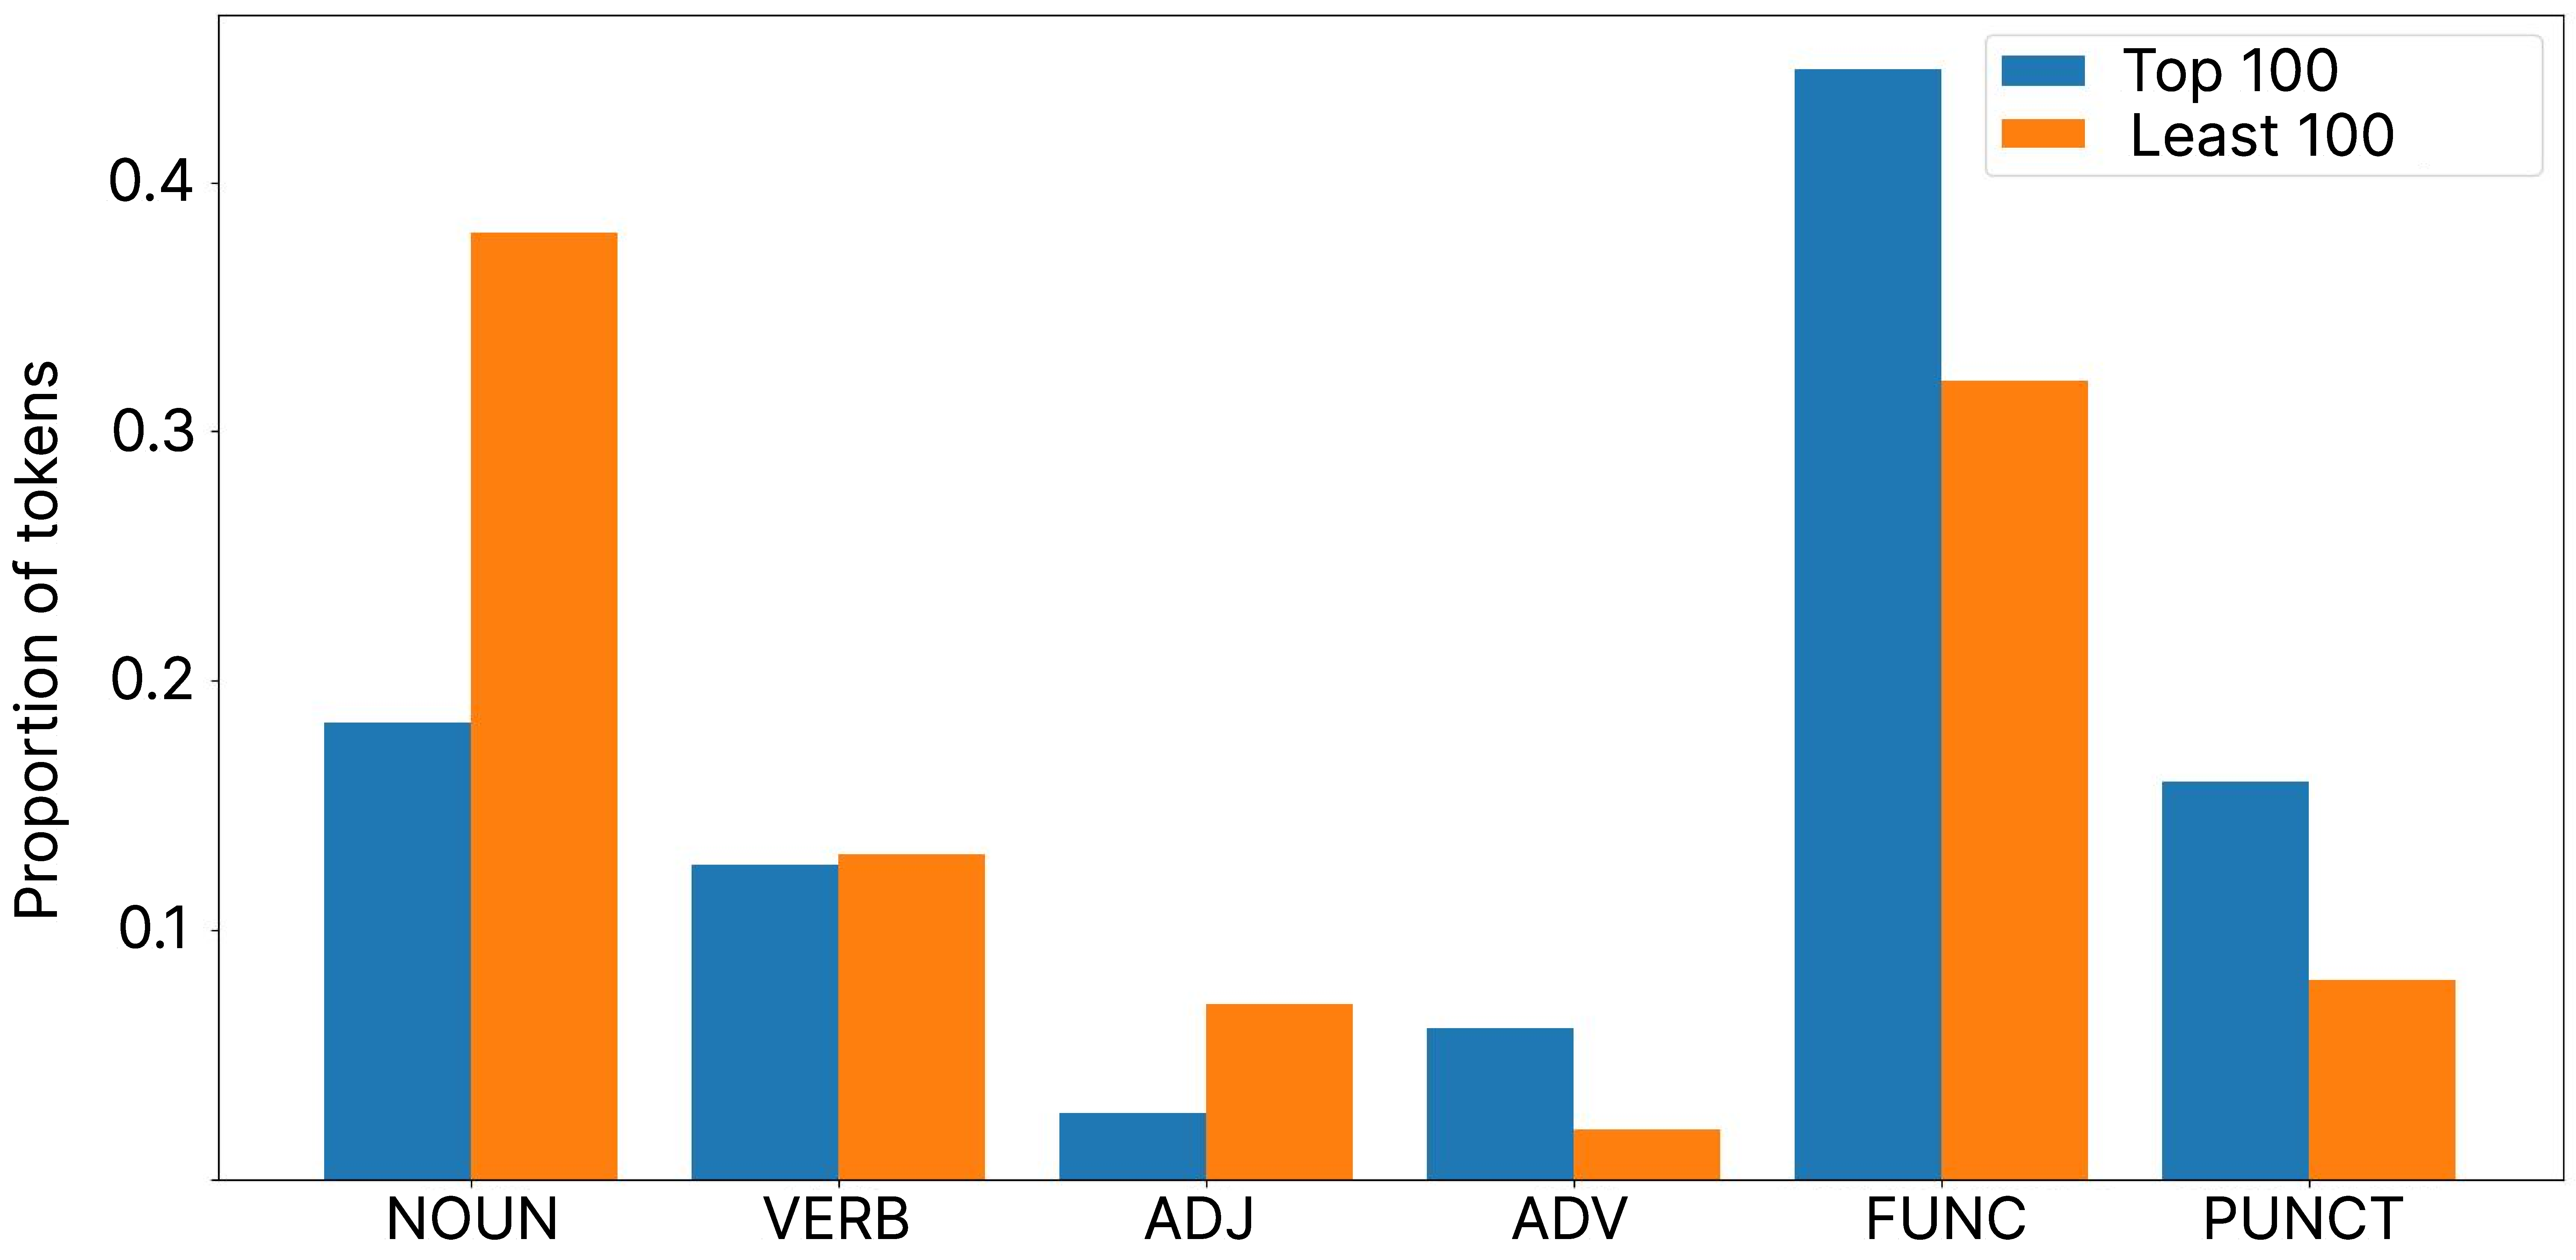
\includegraphics[height=4cm]{chapters/chapter 2/figures/top_versus_bottom_pos_dist.png}
    \caption{Distribution across POS tags of the top versus bottom 100 most frequent tokens.}
    \label{fig:top-100-pos-dist}
\end{figure}

\section{BLiMP Data Filtering}
\label{section:appendix-data-filtering}

We filter the BLiMP data to only focus on pairs of sentences where one set of tokens has been replaced by another set and ignore sentence pairs that only differ in the order of tokens. We also remove pairs where tokens have only been added to one sentence, rather than replaced. This filtering only removes 15\% of BLiMP pairs and 9 of the 67 subtasks from consideration. 

\section{NLU Performance of Open-Source Baselines}
\label{section:opensource-baselines-nlu-results}

\begin{table}[ht!]
\centering
\small
\setlength{\tabcolsep}{5pt} % Adjust column separation
\begin{tabular}{l|c|cccc}
\toprule
\textbf{Model} & \textbf{BLiMP} & \textbf{COLA} & \textbf{SST-2} & \textbf{MNLI} & \textbf{QNLI} \\
\midrule
OPT & 63.2 & 64.6 & 81.9 & 57.6 & 61.5 \\
RoBERTa & 69.8 & 70.8 & 87.0 & 73.2 & 77.0 \\
T5 & 58.3 & 61.2 & 78.1 & 48.0 & 62.0 \\
\bottomrule
\end{tabular}
\caption{\label{tbl:opensource-baselines-nlu-results} BLiMP~($\uparrow$) score and accuracy ($\uparrow$) on sentence-level tasks (COLA, SST-2) and language inference tasks (MNLI, QNLI) for the three open-source transformer baselines.}
\end{table}

\chapter{Tending Towards Stability: Convergence Challenges in Small Language Models}
\label{chapter:tending-towards-stability}

Large-scale language models (LMs) have driven recent breakthroughs in natural language processing, demonstrating remarkable performance across a range of tasks \citep{hendrycks2021mmlu, chowdhery2023palm}. These gains are largely attributed to scale: increasing model size has become the dominant paradigm for improving performance. However, large models come with steep computational and environmental costs \citep{schwartz2020greenai}, making them less accessible and less practical in many real-world settings.

Small language models offer a more sustainable and democratized alternative, enabling training on proprietary or domain-specific data, improving privacy, and reducing deployment costs \citep{huang2022large, bender2021dangers}. Yet despite their advantages, small models often lag significantly behind their larger counterparts—not only in final performance, but in the learning process itself. Empirical studies have observed that small models tend to degrade in performance late in pretraining, a phenomenon known as saturation \citep{godey2024small}. While this behavior is often attributed to limited representational capacity, the precise learning dynamics that give rise to these failures remain poorly understood.

In this chapter, we build on the analytical frameworks introduced in Chapter 5 and provide a detailed investigation into the convergence behavior of language models across scales. Specifically, we focus on how internal representations—especially the outputs of attention and feedforward layers—evolve during training. We use tools like Centered Kernel Alignment (CKA) and a new metric we term Proportional Effective Rank (PER) to examine how quickly and smoothly different layers in a model converge to their final state, and how this varies with model size.

Using the Pythia model suite \citep{biderman2023pythia}, which offers consistent training checkpoints across a range of model sizes, we show that larger models exhibit faster and more monotonic convergence in their internal activations. In contrast, smaller models show delayed and more erratic convergence, particularly in deeper layers. We find that these differences correlate with the effective rank of each layer’s parameters and gradients—suggesting that small models not only struggle to converge, but also tend to use a narrower subspace of their available capacity throughout training.

These findings offer a new lens on training inefficiency in small models and help formalize how and why learning breaks down as scale decreases. They also motivate new directions for improving small models, such as targeted interventions that increase effective rank or promote smoother convergence dynamics.

\paragraph{Contributions.}
Our main contributions are as follows:
\begin{enumerate}
    \item We perform a detailed convergence analysis of attention and MLP layer activations across models ranging from 70M to 2.8B parameters. We show that larger models converge faster and more smoothly to their final representations.

    \item We introduce the metric of Proportional Effective Rank (PER) to compare how efficiently models use their parameter space, adjusting for differences in model size.

    \item We find that layers with higher PER values (in both weights and gradients) tend to converge earlier, revealing a strong correlation between representational richness and learning stability.

    \item We highlight that small models underutilize their representational space during training, leading to slower convergence and increased instability in deeper layers.
\end{enumerate}

In the following sections, we define our methodology, describe our empirical setup, and present results that reveal systematic differences in how large and small models learn—and how these differences may ultimately explain the persistent performance gap.


\section{Methodology and Analytical Framing}
\label{sec:methodology}

To better understand training inefficiencies in small language models (LMs), we examine how internal representations evolve during pretraining across model sizes. Our analysis focuses on the \textit{residual stream}---the central information pathway in transformers---and tracks both activation dynamics and parameter behavior through the lens of representation similarity and dimensionality metrics. 

This section outlines the analytical tools we use and how they allow us to quantify differences in convergence patterns across layers and model scales.

\paragraph{Residual Stream and Layer Updates.}
Each layer in a transformer updates the model's residual stream by composing two subcomponents: multi-head self-attention ($\attention$) and a feedforward network ($\mlp$). These updates can be expressed as:
\begin{align}
    \xdata' &= \xdata_{\layer-1} + \attention(\xdata_{\layer-1}) \\
    \xdata_{\layer} &= \xdata' + \mlp(\xdata')
\end{align}
where $\xdata_{\layer} \in \mathbb{R}^{\seqlen \times \residualdim}$ denotes the residual stream after layer $\layer$. The residual stream provides a continuous trace of how information is transformed as it flows through the network.

Each subcomponent writes back to the residual stream via parameterized projections: $\attention$ updates involve low-rank writes using output matrices $W_O W_V$ per attention head, while $\mlp$ uses a full-rank transformation. This structure underpins our focus on the write operations from both $\attention$ and $\mlp$ as the locus of learning dynamics.

\paragraph{Activation Convergence via CKA.}
To quantify how each layer's representation stabilizes during training, we compute the similarity of its activations over time using the Centered Kernel Alignment (CKA) metric \citep{kornblith2019cka}. For a given layer $\layer$, we compare the activations at checkpoint $t$ to those at the final checkpoint $T$:
\begin{align}
    \cka(\actcenter_{t}, \actcenter_{T}) = 
    \frac{\|\actcenter_{t}^{\top} \actcenter_{T}\|_F^2}
         {\|\actcenter_{t}^{\top} \actcenter_{t}\|_F \cdot \|\actcenter_{T}^{\top} \actcenter_{T}\|_F}
\end{align}
where $\actcenter$ denotes mean-centered activations and $\|\cdot\|_F$ is the Frobenius norm. Higher CKA values indicate greater similarity, reflecting convergence toward a layer's final activation behavior.

While CKA and related metrics (e.g., SVCCA) have been widely used to study representational similarity \citep{wu2020similarity, phang2021finetuned, brown2023understanding}, we adapt this tool to a new setting: analyzing the temporal dynamics of activation convergence across model sizes, rather than comparing across models or tasks.

\paragraph{Parameter Structure via Proportional Effective Rank.}
We further analyze the expressivity of each layer by computing the \textit{effective rank} of its write parameters—the projection matrices that return intermediate representations to the residual stream. The effective rank of a matrix $\vtheta \in \mathbb{R}^{d \times h}$ is defined as the entropy of its normalized singular values \citep{roy2007effectiverank}:
\begin{align}
    \er(\vtheta) = \exp\left(-\sum_{k=1}^K \frac{\sigma_k}{\|\sigma\|_1} \log \frac{\sigma_k}{\|\sigma\|_1}\right)
\end{align}
To facilitate comparisons across models of varying sizes, we normalize this quantity by the number of hidden dimensions $h$, resulting in the \textbf{Proportional Effective Rank (PER)}:
\begin{align}
    \per(\vtheta) = \er(\vtheta) / h
\end{align}
We compute PER for both weight matrices ($\vtheta$) and their gradients ($\nabla \vtheta$), capturing how richly each layer utilizes its capacity and how broadly learning signals are distributed during training. Intuitively, a higher PER indicates that a layer operates across a more diverse subspace of its available dimensions—rather than collapsing into a narrow, low-rank direction—suggesting more expressive updates and reduced redundancy. This makes PER a useful diagnostic for identifying inefficiencies in learning: when PER is low, it implies that despite having many parameters, a layer may not be effectively leveraging its full representational capacity.


\paragraph{Novel Analytical Angle.}
While prior work on small model saturation has largely focused on representational limitations at the output layer \citep{godey2024small, yang2018breaking}, our study introduces a new perspective: we examine convergence inefficiencies earlier in the network. By connecting convergence dynamics (via CKA) with representational underutilization (via PER) throughout the entire network, we identify specific structural bottlenecks that arise during training—especially in smaller models.

These tools allow us to pose and answer key questions: Do different-sized models converge at the same rate across layers? Are slower convergence dynamics associated with lower-rank parameter usage? And can these insights inform better training or design strategies for small language models?



% % ============
% % RELATED WORK
% % ============
% \section{Related Work}\label{sec:related_work}

% Prior work has studied various learning dynamics of the Pythia suite, including memorization \citep{biderman2023pythia, lesci2024causal}, training data influence \citep{chai2024training}, and statistics of learned embeddings \citep{belrose2024neural}.
% Related to our work, \citet{godey2024small} examine the differences in the rank of the unembedding matrix (mapping from hidden representations to tokens) across model sizes, known as the softmax bottleneck \citep{yang2018breaking}. Unlike their findings, we focus on the convergence dynamics of all layers.

% Similarity metrics like $\cka$ and Singular Vector Canonical Correlation Analysis (SVCCA) are widely used to analyze language model properties. \citet{nguyen2020wide} find that architectural decisions, such as model width and depth, affect hidden representation similarity. \citet{wu2020similarity} show that models within the same architectural family share similar hidden structures, a similarity that persists even in fine-tuned models \citep{phang2021finetuned}. Additionally, SVCCA has been used to study token representation distribution in multilingual models \citep{singh2019bert} and syntactic element learning in monolingual models \citep{saphra2019understanding}.
% Most similar to our work, \citet{brown2023understanding} use representation similarity metrics, including $\cka$, to study Pythia generalization capabilities. However, our study is the first to use the $\cka$ metric to examine the convergence dynamics of layers' activations across model sizes.


% % ===========
% % METHODOLOGY
% % ===========
% \section{Methodology}\label{sec:methodology}

% We first describe the residual stream view of transformer-based models and define layers' activations. Then, we introduce the $\cka$ and proportional effective rank metrics.

% \paragraph{The \textit{Residual Stream} view.}
% The residual stream view of the transformer architecture \citep{vaswani2017attention} is an analytical framework to study how information flows through its layers \citep{elhage2021mathematical}. 
% This conceptualization focuses on the residual connections as they provide a direct reference to the inputs. Specifically, the set of residual connections across layers is termed the \defn{residual stream}. Each layer can be seen as providing modifications to the residual stream via addition operations.
% Layers have two main components, $\attention$ and $\mlp$, that sequentially update the residual stream. Formally, a sequence of $\seqlen$ tokens, $\sequence = \langle \token_1, \smalldots, \token_\seqlen\rangle$ is first converted into a matrix $\xdata_0 \mathop{\in} \R^{\mathop{\seqlen\times\residualdim}}$ by the embedding layer: each column is a token representation of size $\residualdim$. Then, each layer $\layer\mathop{\in}\{1,\smalldots, \numlayers\}$ updates these representations as follows:
% \begin{align}\label{eq:residual_stream}
%     \xdata' &= \xdata_{\layer-1}  + \dashuline{\attention(\xdata_{\layer-1})} \\
%     \xdata_\layer &= \xdata' + \dashuline{\mlp(\xdata')}
% \end{align}
% Finally, the $\seqlen$-th column of $\xdata_\numlayers$ is used to predict the $(\seqlen\mathop{+}1)$-th token. 

% The residual stream is a mathematical formalization through which to study how transformer models process inputs \citep{elhage2021mathematical}. Under this framework, each of the $L$ layers of a transformer model processes a series of input tokens $\sequence = \langle \token_1, \smalldots, \token_\seqlen\rangle$ consecutively and communicate the result of their computation for each token to subsequent layers via a residual stream of dimension $\residualdim$. 
% The reading, processing, and writing of the residual stream occur independently in each $\attention$ head via combinations of the query, key, value and output matrices, $W_Q$, $W_K$, $W_V$, $W_O$: The \textbf{query-key circuit}, $W_Q^{\top}W_K$, of the $\attention$ mechanism controls how the residual stream should be recomposed, and the \textbf{output circuit}, $W_OW_V$, writes to the residual stream an update that is mediated by the query-key circuit. The write operation of each $\attention$ head is of low rank relative to $\residualdim$. After each $\attention$ head has written to the residual stream, a bottleneck $\mlp$ projection performs a full-rank transformation on the residual stream.  Due to their pivotal role in updating the state of the residual stream, our work analyses the learning dynamics of the two operations that write to the residual stream: the output circuit of each head of the $\attention$ layer---that we refer to as $\attention$---and the $\mlp$ projection layer---that we denote $\mlp$ for conciseness.


% \paragraph{\textit{Activations} and \textit{Parameters}.}
% The updates to the residual stream---\dashuline{underlined} in \cref{eq:residual_stream}---are the layer's \defn{activations} and have the same dimensions as the residual stream, i.e., $\R^{\mathop{\seqlen\times\residualdim}}$. Both $\attention$ and $\mlp$ first project, or \enquote{read}, the residual stream into lower-dimensional intermediate representations; then project these representations back, or \enquote{write}, into the residual stream. Here, we study the behavior of the \defn{parameters} that write to the residual stream.
% We use $\actatt$ and $\actmlp$ to denote the activations and $\attweight$ and $\mlpweight$ to denote the parameters of, respectively, $\attention$ and $\mlp$.

% \paragraph{Activations' Similarity.}
% Given a set of activations, either $\actatt$ or $\actmlp$, of a layer $\layer$ at a particular checkpoint $\checkpoint$, $\act_{\layer, \checkpoint}$, we measure how similar they are to those at the last checkpoint $\numcheckpoints$, $\act_{\layer, \numcheckpoints}$, using the linear variant of the Centered Kernel Alignment metric \citep[$\cka$;][]{kornblith2019cka}:
% \begin{align}\label{eq:cka}
%     \cka(\actcenter_{\checkpoint}, \actcenter_{\numcheckpoints}) = \frac{\norm{\actcenter_{\checkpoint}{}^{\top}\, \actcenter_{\numcheckpoints}}^2_F}{\norm{\actcenter_{\checkpoint}{}^{\top}\,\actcenter_{\checkpoint}}_F\; \;\norm{\actcenter_{\numcheckpoints}{}^{\top}\,\actcenter_{\numcheckpoints}}_F}
% \end{align}
% where $\actcenter$ denotes the centered activations, and $\norm{\cdot}_F$ is the Frobenius norm; we omit the layer subscript $\layer$ for clarity.
% We compute \cref{eq:cka} for both $\actatt$ and $\actmlp$ across all layers and checkpoints throughout training, allowing us to examine the convergence dynamics of each layer's activations.

% \paragraph{Parameters' \textit{Proportional Effective Rank}.}
% Let $\hiddendim$ be the dimension of the intermediate representation of either $\attention$ or $\mlp$. For a layer $\layer$, let $\vtheta_{\layer} \in \R^{\mathop{\residualdim\times\hiddendim}}$ be the subset of parameters of either $\attweight$ or $\mlpweight$ that comprise the matrix that projects from the hidden space into the residual stream.
% We measure the effective number of dimensions onto which $\vtheta_{\layer}$ projects the intermediate representations using the definition of  \defn{effective rank} introduced in \citet{roy2007effectiverank}. The effective rank is computed as the entropy over the normalised singular values of the parameter matrix $\vtheta_{\layer}$, that is:
% \begin{align}\label{eq:per}
%     \er(\vtheta_{\layer}) = \exp \left( -\sum_{k=1}^K \frac{\sigma_k}{\norm{\sigma}_1} \; \log \frac{\sigma_k}{\norm{\sigma}_1}\right)
% \end{align}
% where $\sigma = \langle\sigma_1, \smalldots, \sigma_K\rangle$ is the vector of singular values and $\norm{\cdot}_1$ is the $\ell_1$ norm.
% In this paper, we introduce the notion of a \defn{proportional effective rank} ($\per$) computed as the effective rank normalized by the number of hidden dimensions: 
% \begin{align}
%     \per(\vtheta_{\layer}) = \er(\vtheta_{\layer}) \, / \, \hiddendim
% \end{align}
% The $\per$ allows us to compare the effective rank of layers with different sizes consistently. We compute the $\per$ of both $\attweight$ and $\mlpweight$, as well as the gradients of these parameters, across all layers and checkpoints throughout training. 



% ==================
% EXPERIMENTAL SETUP
% ==================
\section{Experimental Setup}\label{sec:experimental_setup}

We use the Pythia model suite \citep{biderman2023pythia}, composed of \integer{8} transformers of different sizes trained for \q{143}{\thousand} steps on the deduplicated\footnote{There exists a non-deduplicated (or standard) version of the Pile dataset used to train a first version of the Pythia suite.} version of the Pile dataset \citep{gao2020pile}.
Intermediate checkpoints are available every \q{1}{\thousand} steps and at log-spaced intervals early in training.
To comply with our computational budget, we consider models up to \q{2.8}{\billion} parameters---i.e., \sevenmil, \sixmil, \fourmil, \onebil, and \twobil---evaluated at the following steps: \integer{0}, all log-spaced steps $\{1, 2, 4, \smalldots, 512\}$, \q{1}{\thousand}, \q{3}{\thousand}, and then every \q{10}{\thousand} steps up to \q{143}{\thousand}.
We evaluate each checkpoint on the last batch of the training set and collect its activations.

We use the publicly available Pythia model suite \citep{biderman2023pythia}, which was trained on the Pile \citep{gao2020pile}. Both the preprocessed training data and intermediate checkpoints are publicly available.\footnote{\href{https://github.com/EleutherAI/pythia}{\myemph{github.com/EleutherAI/pythia}} (Apache License 2.0).} 

\paragraph{Data.}
The Pile is a \q{300}{\billion}-token curated open-source collection of English documents, spanning a wide range of domains (e.g. books, academic publications, Wikipedia). \footnote{\href{https://github.com/EleutherAI/the-pile}{\myemph{github.com/EleutherAI/the-pile}} (MIT License).}  
The deduplicated version of the dataset is obtained by applying a near-deduplication method based on \myemph{MinHashLSH} and has \q{207}{\billion} tokens.
Thus, models trained on this version of the dataset are trained for circa \float[1]{1.5} epochs to keep an equal token count relative to the non-deduplicated versions.
The dataset is shuffled, tokenised, and \enquote{packed} into sequences of \integer{2049} tokens with no end-of-document token\footnote{\href{https://github.com/EleutherAI/pythia/issues/123}{\myemph{github.com/EleutherAI/pythia/issues/123}}.}.
Noticeably, the packing process implies that the second half-epoch of deduplicated data contains the same documents but not necessarily the same sequences. 
By design, each sequence can pack multiple documents and tokens can attend across document boundaries.

\paragraph{Models.}
The Pythia model suite is composed of 16 models: transformers of \integer{8} different sizes trained on the Pile as-is and deduplicated.
All model sizes were trained using a cosine learning rate schedule with warm-up, the same data order, and a batch size of \integer{1024} sequences, resulting in exactly \q{143}{\thousand} optimization steps.
Checkpoints are available at initialization (step \integer{0}), and after every \q{1}{\thousand} iterations (steps \q{1}{\thousand}-\q{143}{\thousand}) resulting in \integer{144} checkpoints evenly spaced throughout training. 
Additionally, log-spaced checkpoints are available early in training (steps $\{2^i\}_{i=0}^{9}$). In \cref{tab:model_hparams} we report more details about the architecture and training hyper-parameters of the models in the suite.

\begin{table}[!t]
    \centering
    \begin{tabular}{lcccccc}
    \toprule
    \textbf{Size} & $\numlayers$ & $\residualdim$ & \textbf{\# Heads} & \textbf{Batch Size} & \textbf{Learning Rate} & \textbf{Checkpoints} \\
    \midrule
    \sevenmil & \integer{6} & \integer{512} & \integer{8} & \q{2}{\million} & \snum{1e-3} & \href{https://huggingface.co/EleutherAI/pythia-70m}{\myemph{Standard}}, \href{https://huggingface.co/EleutherAI/pythia-70m-deduped}{\myemph{Deduped}} \\
    \sixmil & \integer{12} & \integer{768} & \integer{12} & \q{2}{\million} & \snum{6e-4} & \href{https://huggingface.co/EleutherAI/pythia-160m}{\myemph{Standard}}, \href{https://huggingface.co/EleutherAI/pythia-160m-deduped}{\myemph{Deduped}} \\
    \fourmil & \integer{24} & \integer{1024} & \integer{16} & \q{2}{\million} & \snum{3e-4} & \href{https://huggingface.co/EleutherAI/pythia-410m}{\myemph{Standard}}, \href{https://huggingface.co/EleutherAI/pythia-410m-deduped}{\myemph{Deduped}} \\
    \onebil & \integer{24} & \integer{2048} & \integer{16} & \q{2}{\million} & \snum{2e-4} & \href{https://huggingface.co/EleutherAI/pythia-1.4b}{\myemph{Standard}}, \href{https://huggingface.co/EleutherAI/pythia-1.4b-deduped}{\myemph{Deduped}} \\
    \twobil & \integer{32} & \integer{2560} & \integer{32} & \q{2}{\million} & \snum{1.6e-4} & \href{https://huggingface.co/EleutherAI/pythia-2.8b}{\myemph{Standard}}, \href{https://huggingface.co/EleutherAI/pythia-2.8b-deduped}{\myemph{Deduped}} \\
    \bottomrule
\end{tabular}
    
    \caption{Details on the architecture and training hyper-parameters for models in the Pythia suite used in this paper. $\numlayers$ is the number of layers, $\residualdim$ is the dimension of the residual stream. The number of hidden dimensions per head is simpl the number of heads divided by the number of dimensions in the residual stream.}
    \label{tab:model_hparams}
\end{table}


% =======
% RESULTS
% =======
\section{Results}
\label{sec:tending-towards-stability-results}

Our analysis reveals systematic differences in the learning dynamics of transformer layers across model scales. We study these dynamics through two complementary lenses: the convergence behavior of layer activations and the proportional effective rank ($\per$) of layer parameters and their gradients. Together, these measures provide insight into how layers develop and utilize capacity over time during training.

\begin{wrapfigure}{r}{0.6\columnwidth}
    \centering
    \includegraphics[width=0.58\columnwidth]{chapters/tending-towards-stability/figures/cka_main_plot.pdf}
    \caption{$\cka$ similarity (current vs.\ last checkpoint) of $\attention$ and $\mlp$ activations for Pythia \sixmil and \twobil. Distribution across layers: \integer{10}, \integer{25}, \integer{50}, \integer{75}, and \integer{90}-th percentiles per checkpoint.}
    \label{fig:cka_main_plot}
\end{wrapfigure}

Before presenting our detailed analyses, we briefly describe the structure of the main figures. \cref{fig:main-results} summarizes our core findings across three axes: (1) the convergence of activations as measured by $\cka$ similarity to final checkpoint activations (first column), (2) the proportional effective rank ($\per$) of layers' parameters (second column), and (3) the $\per$ of the corresponding parameter gradients (third column). Each row shows statistics for a different operation—$\attention$ (top) and $\mlp$ (bottom)—and each line represents the mean value across layers for five Pythia models ranging from 70M to 2.8B parameters.

In addition to these averaged results, \cref{fig:cka_main_plot} displays the inter-quartile range of $\cka$ similarity values averaged across layers for the smallest and largest models, and \cref{fig:cka-layer-wise-lines}, \cref{fig:per_weight-layer-wise-lines}, and \cref{fig:per_grad-layer-wise-lines} provide a layer-wise breakdown of convergence and rank dynamics (for both weights and gradients), respectively. These figures allow us to distinguish aggregate trends from layer-specific behaviors and to track how representational capacity and learning signals evolve during training.

\clearpage

\begin{figure*}[h!]
    \centering
    \includegraphics[width=0.9\linewidth]{chapters/tending-towards-stability/figures/cka_full_lines.pdf}
    \vspace{-5pt}
    \caption{$\cka$ similarity (current vs last checkpoint) of the activations of $\attention$ and $\mlp$ in each layer of Pythia \q{70}{\million}, \q{160}{\million}, \q{410}{\million}, \q{1.4}{\billion} and \q{2.8}{\billion} throughout training.}%
    \label{fig:cka-layer-wise-lines}
\end{figure*}
\clearpage

\begin{figure*}[h!]
    \centering
    \includegraphics[width=0.9\linewidth]{chapters/tending-towards-stability/figures/per_weight_lines.pdf}
    \vspace{-5pt}
    \caption{$\per$ of the weight matrices of $\attention$ and $\mlp$ in each layer of Pythia \q{70}{\million}, \q{160}{\million}, \q{410}{\million}, \q{1.4}{\billion} and \q{2.8}{\billion} throughout training.}%
    \label{fig:per_weight-layer-wise-lines}
\end{figure*}
\clearpage

\begin{figure*}[h!]
    \centering
    \includegraphics[width=0.9\linewidth]{chapters/tending-towards-stability/figures/per_grad_lines.pdf}
    \vspace{-5pt}
    \caption{$\per$ of the gradients of the weight matrices of $\attention$ and $\mlp$ in each layer of Pythia \q{70}{\million}, \q{160}{\million}, \q{410}{\million}, \q{1.4}{\billion} and \q{2.8}{\billion} throughout training.}%
    \label{fig:per_grad-layer-wise-lines}
\end{figure*}
\clearpage



\begin{result}[Activations of larger models converge faster and more monotonically to their final state than those of smaller models]
\label{result:cka}


As shown in the first column of \cref{fig:main-results}, $\cka$ similarity between a layer's activations at a given checkpoint and its final state rises more quickly in larger models. For instance, by 20\% of training, the $\cka$ score in \twobil reaches $\sim$0.8 for $\mlp$ and $\sim$0.7 for $\attention$, compared to values around 0.5 in \sevenmil and \sixmil. This trend reflects more rapid and stable convergence.

\cref{fig:cka_main_plot} adds further evidence: across checkpoints, the interquartile range (25th to 75th percentiles) of $\cka$ similarity across layers is both narrower and higher in larger models, confirming convergence is more uniform layer-wise.

\cref{fig:cka-layer-wise-lines} provides a more granular, layer-wise view: in \twobil, many layers—especially earlier ones—achieve high similarity early in training, whereas in smaller models convergence is delayed and less monotonic.

% As observed in \cref{fig:main-results} (first column), larger models show, on average, earlier convergence of $\attention$ and $\mlp$ activations. For example, by \q{20}{\percent} of training, the $\cka$ score in \twobil is \float[1]{0.8} for $\mlp$ and \float[1]{0.7} for $\attention$, where in \sevenmil and \sixmil it is around \float[1]{.5}.
% This fast convergence pattern holds across layers, as shown by the distributions in \cref{fig:cka_main_plot}.
\end{result}

\begin{result}[Activations of earlier layers converge faster, regardless of the model size]
Across model sizes, earlier layers' activations converge faster to their final state than those of later layers. As shown in \cref{fig:cka-layer-wise-lines}, the faster average convergence in larger models is due to more of their later layers converging earlier, whereas smaller models' layers only reach their final state towards the end of training.
\end{result}

\vspace{9pt}
Based on recent work that identifies parameter rank differences across model sizes \citep{godey2024small}, in the next paragraphs, we study whether the different convergence behaviours are related to the effective rank of layers' parameters and gradients.
\vspace{9pt}

\begin{result}[Parameters of layers in larger models proportionally span more dimensions] 
\label{result:weight-effective-rank} 
Parameters in layers of larger models span a slightly larger fraction of their available dimensions compared to smaller models, as shown in \cref{fig:main-results} (second column). 
Moreover, the $\per$ of larger models stabilises early, while it keeps decreasing throughout training for smaller ones. This finding is further underscored when visualising the $\per$ for each layer, as shown in \cref{fig:per_weight-layer-wise-lines}; we observe that in smaller models the $\per$ of later layers tends to decrease over the course of training, while in larger models the $\per$ of all layers stabilises early in training. This difference is even more pronounced in the $\per$ of these layers' gradients, as shown in \cref{fig:main-results} (third column).
\end{result}

\begin{result}[Parameters of layers in larger models receive gradient updates along proportionally more dimensions]
\label{result}
The $\per$ of gradients reflects the proportion of the learning signal transmitted by the gradients relative to the available parameter dimensions. In \cref{fig:main-results} (third column), we observe that throughout training gradients in larger models consistently span a larger fraction of the available dimensions, with this fraction gradually decreasing over time. In contrast, smaller models display more variability. At first glance, the averaged $\per$ of gradients in the $\attention$ layer of the \twobil model might appear to contradict the observed trend. However, this discrepancy is clarified when examining the $\per$ of gradients across individual layers, as shown in \cref{fig:per_grad-layer-wise-lines}. Once again, we observe that the $\per$ of gradients in later layers of smaller models are less stable compared to larger models. The reason the average $\per$ of gradients in the $\attention$ layer of the \twobil model is smaller than in smaller models is that, early in training, all layers of the larger model stabilise at their final values. At this stage, the stabilised layers of the larger model have lower gradient $\per$ values compared to those of smaller models, which have not yet converged. Overall, our findings suggest that layers in larger models converge both more quickly and tend to receive proportionally larger rank updates during training.
\end{result}


\begin{figure*}[h!]
    \centering
    \includegraphics[width=\linewidth]{chapters/tending-towards-stability/figures/results.pdf}
    \vspace{-15pt}
    \caption{$\cka$ similarity (current vs.\ last checkpoint) of layers' activations (first column), $\per$ of layers' parameters (second column) and gradients (third column) for $\attention$ (top row) and $\mlp$ (bottom row) in Pythia \sevenmil, \sixmil, \fourmil, \onebil, and \twobil averaged (mean) across layers per each checkpoint.}
    \label{fig:main-results}
\end{figure*}


\begin{result}[The dynamics of the parameters' effective rank and the activations' convergence patterns are correlated]
We investigate the correlation between a layer's activations convergence rate and the rank of its parameters and gradients. Broadly, we find that layers with higher effective rank in both weights and gradients converge faster.
To measure this correlation, we first create two binary variables for each layer indicating whether (i) it converges early in training and (ii) maintains a stable $\per$ throughout training. Then, we calculate the Matthew's Correlation Coefficient between these two statistics across layers and report them in \cref{tab:model_correlation}.
Specifically, for each layer of a given model, we determine whether that layer exhibits early activations' convergence and large and stable parameters' and gradients' $\per$s (relative to other model layers) using the following heuristics: 
\begin{itemize}
    \item \textbf{Early activations' convergence.} Activations' $\cka \mathop{\geq} \float[2]{0.45}$ by the first \q{10}{\percent} of training (applies to both the $\attention$ and $\mlp$ layers).
    
    \item \textbf{Large parameters' $\per$.} Parameters' $\per \mathop{\geq} \float[2]{0.95}$ by the end of training (applies to both the $\attention$ and $\mlp$ layers).
    
    \item \textbf{Large gradients' $\per$.} We note that gradients' $\per$ slightly decreases throughout training for each model size. Rather than choosing a fixed value to determine large and stable gradients' $\per$s, we dynamically set the threshold at \q{90}{\percent} of the largest $\per$ attained by any layer at the end of training.
\end{itemize}
We observe a strong correlation for the $\attention$ layers across model sizes. For the $\mlp$ layers, the correlation with the gradients' $\per$ is strong for models up to \onebil, while the correlation with the parameters' $\per$ is strong only for the \sevenmil model. We hypothesize that this discrepancy can be explained by the fact that $\mlp$ layers have a large $\per$ throughout training across all model sizes, apart from those of the \sevenmil model. 

While these results are correlational, they provide a foundation for future work to test whether methods that specifically increase the PER of layers' parameters and gradients induce faster convergence of the layers' activations in small models.
\end{result}

\begin{table}[!t]
    \centering
    \begin{tabular}{crrrr}
\toprule
 \textbf{Size} & $\attweight$  & $\nabla \attweight$ & $\mlpweight$ & $\nabla\mlpweight$\\ 
\midrule
\sevenmil  & \float[2]{1.000} & \float[2]{1.000} & \float[2]{0.632} & \float[2]{1.00} \\ 
\sixmil & \float[2]{1.000} & \float[2]{0.845} & \float[2]{0.357} & \float[2]{0.714} \\ 
\fourmil & \float[2]{0.837} & \float[2]{0.916} & \float[2]{0.192} & \float[2]{0.777} \\ 
\onebil & \float[2]{0.775} & \float[2]{0.845} & \float[2]{0.209} & \float[2]{0.641} \\ 
\twobil & \float[2]{0.728} & \float[2]{0.521} & \float[2]{0.112} & \float[2]{0.179} \\ 
\bottomrule
\end{tabular}
    \caption{Matthew's Correlation Coefficient %($\phi$)
    between binary variables indicating whether a given layer converges early in training and whether it maintains a stable PER of the parameters ($\vtheta$) and gradients ($\nabla\vtheta$) throughout training for both $\attention$ and $\mlp$.}
    \label{tab:model_correlation}
\end{table}



% ===========
% CONCLUSIONS
% ===========
\section{Conclusion}

Our findings reveal consistent and interpretable distinctions in learning dynamics across model scales. Larger models exhibit faster and more monotonic convergence in their layer activations, and make fuller use of their representational capacity; this is evidenced by higher and more stable proportional effective ranks ($\per$) of both weights and gradients. In contrast, smaller models display delayed convergence, greater instability, and under-utilization of available capacity. These patterns suggest that part of the capability gap between small and large models may stem not from optimization failure per se, but from inefficient or truncated learning trajectories.

Importantly, these insights offer actionable hypotheses: for instance, that inducing higher-rank updates or more distributed gradient flows might help smaller models converge more like their larger counterparts. However, testing such hypotheses directly, for instance by intervening on training dynamics and re-evaluating learning behavior, is difficult in practice.

Ideally, we would now like to modify the Pythia models (for example, to encourage higher effective rank early in training) and retrain them to see whether convergence patterns improve. Yet retraining Pythia is non-trivial. There are several practical limitations:

\begin{itemize}[label=\xmark]
    \item \textbf{The dataset (the Pile)} is not easily streamable in its deduplicated format, and lacks a flexible preprocessing pipeline. Simply downloading the dataset is non-trivial because it requires a large amount of disk space and running a custom preprocessing script.
    \item \textbf{The model and training code requires Megatron-DeepSpeed}, which introduces heavy engineering overhead, tightly coupled dependencies, and strict hardware requirements. This additionally makes reading the code and intervening in the model architecture and training pipeline cumbersom.
    \item \textbf{The training pipeline is distributed in Docker environments} with kubernetes for large-scale distributed training. Although this is good engineering practice in industry, these tools add overhead and complexity that is not necessary for small-scale research.
    \item \textbf{Checkpointing is limited to weights}, meaning that intermediate activation or gradient states of the model are missing, and difficult to recover. For instance, it is not obvious how to determine the exact set of data that was seen by the model at a given checkpoint which would be necessary to reproduce the activations at that checkpoint.
    \item \textbf{Pythia checkpoints do not natively plug in with analysis libraries}, making it difficult to use existing analysis tools to study learning dynamics.
\end{itemize}

To rigorously study learning dynamics, and in particular, to test targeted training interventions, we need a framework that makes model retraining as accessible as analysis. Such a framework should:

\begin{tcolorbox}[
    colback=white,
    colframe=thesisblue,
    title=\textbf{Design Requirements for Intervention-Friendly Language Model Platforms},
    fonttitle=\bfseries,
    coltitle=white,
    arc=0mm,
    boxrule=1pt,
    left=10pt,
    right=10pt,
    top=10pt,
    bottom=10pt,
    enhanced,
    breakable
]
To effectively support intervention-based research on language model training dynamics, an ideal platform should meet the following criteria:

\begin{itemize}[label=\cmark]
    \item \textbf{Transparency and Modularity}: Fully open-source with minimal external dependencies. Code should be clean, auditable, and modular to support rapid iteration and debugging.
    
    \item \textbf{Reproducible Training and Evaluation}: Provide ready-to-use scripts and configuration files for full training and evaluation pipelines. Baselines should be reproducible with minimal tuning.
    
    \item \textbf{Streamable and Standardized Data}: Support tokenized datasets in streaming formats with built-in preprocessing, packing, and filtering. Avoid proprietary dataset formats or brittle pipelines.
    
    \item \textbf{Intermediate Checkpointing}: Include well-timed checkpoints (e.g., log-spaced or per epoch) to track learning dynamics. Checkpoints should be saved in consistent formats and compatible with analysis tools.
    
    \item \textbf{Structured Logging}: Capture training statistics, gradients, and loss metrics in structured logs (e.g., JSONL, CSV) to enable downstream learning dynamics analysis.
    
    \item \textbf{Flexible Model Configuration}: Allow for easy experimentation with model size, layer depth, attention mechanisms, and other architectural choices through config files or flags.

    \item \textbf{Automatically Plug-in With Existing Third-Party Tools}: Allow for easy integration with existing third-party tools (HuggingFace, Wandb, etc.) for analysis and visualization.

    
    \item \textbf{Lightweight Hardware Requirements}: Be optimized for small and mid-sized models to enable training and analysis on affordable GPU setups, supporting high-velocity prototyping.
\end{itemize}
\end{tcolorbox}

These requirements motivate the development of \pico: a lightweight, transparent framework designed to close the gap between training and analysis for small language models. In the next chapter, we introduce \pico and illustrate how it enables a full cycle of reproducible training, learning dynamics analysis, and hypothesis-driven interventions.




\chapter{The \picosupabig Framework: A Modular Framework for Hypothesis-Driven Language Model Research}
\label{sec:pico-intro}

The rapid progress of large language models (LLMs) has produced systems that excel at a wide range of natural language tasks, from reasoning and summarization to coding and multilingual translation \citep{hendrycks2021mmlu, cobbe2021gsm8k, srivastava2023bigbench}. Yet this progress has also introduced new challenges: as models grow larger and more complex, they become harder to analyze, diagnose, and refine. Developing language models as a result is typically more of an art than a science.

This chapter introduces \pico, a framework designed to transform language model development from empirical guesswork into a rigorous scientific process. \textbf{Pico} enables researchers to systematically observe learning dynamics, formulate testable hypotheses about model behavior, and iterate on design choices through controlled experimentation. By bridging the gap between training and analysis in a single, accessible framework, \textbf{Pico} makes it possible to build language models in a more principled, hypothesis-driven manner. In 


Existing model development frameworks such as DeepSpeed \citep{rasley2020deepspeed}, Megatron-LM \citep{narayanan2021megatron}, and MosaicML's MPT \citep{mosaic2023mpt} have pushed the boundaries of efficient, large-scale training. However, their emphasis on production performance and throughput often comes at the cost of transparency. Intermediate representations, gradients, and activations are rarely captured in a structured way, and instrumentation for fine-grained interpretability is typically an afterthought. As a result, researchers seeking to study learning dynamics or test training interventions face steep technical overhead.

Conversely, frameworks built for interpretability, including TransformerLens \citep{nanda2022transformerlens}, SAELens \citep{bloom2024saelens}, and ACDC \citep{conmy2023towards}, enable detailed circuit-level analysis but are mostly limited to post-hoc exploration of fully trained models. They rarely support modifications to the training process itself, and when they do, such interventions tend to be tightly coupled to specific checkpoints, architectures, or datasets. Even frameworks explicitly designed for developmental analysis, like DevInterp \citep{devinterpcode}, rely on external checkpointing pipelines and are often decoupled from model training.

To support the growing demand for training-time interpretability—that is, the ability to track and intervene in the learning process as it unfolds—we need a framework that makes the training loop itself an object of study. We need infrastructure that not only logs activations and gradients but also invites experimentation with training interventions, architectural variants, and representational diagnostics. Crucially, this framework should be lightweight and accessible, making it possible to iterate quickly without requiring industrial-scale compute or engineering resources.

\textbf{Pico} is a modular, extensible framework designed to fill this gap. Built for training and analyzing small-to-medium scale models (1M--1B parameters), \textbf{Pico} is engineered to support the scientific methodology demonstrated in the previous chapter: systematic observation, hypothesis generation, controlled experimentation, and iterative refinement. It consists of two components:

\begin{enumerate}
    \item \texttt{pico-train}, a customizable training library that makes it easy to train models from scratch while recording rich internal signals (weights, gradients, activations) at regular checkpoints.
    \item \texttt{pico-analyze}, a companion toolkit for querying, visualizing, and analyzing these signals—designed to integrate smoothly with standard scientific workflows and support user-defined metrics.
\end{enumerate}

Together, these tools make it possible to perform fine-grained, in-situ analysis of how models learn over time, test hypotheses about representation development, and prototype interventions that might improve training outcomes—particularly for small models, where interpretability and efficiency are especially critical.

\textbf{Pico} was built to address a concrete gap identified in the previous chapter: existing suites like Pythia offer rich insights into learning dynamics after training, but lack the flexibility and transparency needed to test interventions during training. The findings from \cref{chapter:tending-towards-stability}—such as the correlation between effective rank and convergence speed—generate specific, testable hypotheses that require tools for systematic experimentation. \textbf{Pico} provides these tools, bringing the same level of rigor to the training process as to post-hoc analysis.

The rest of this chapter is structured as follows. We begin by situating \textbf{Pico} within the broader ecosystem of language model training and interpretability frameworks, reviewing both large-scale production platforms and experimental research toolkits. We then describe the key architectural and design decisions behind \texttt{pico-train} and \texttt{pico-analyze}, highlighting how they support training-time experimentation. Finally, we demonstrate \textbf{Pico}'s value through case studies that show how it enables researchers to systematically test and refine hypotheses about language model learning dynamics.

{
\renewcommand{\arraystretch}{1.25}
\setlength{\tabcolsep}{4pt}

\begin{table}[htbp]
    \centering
    \footnotesize
    \begin{tabular}{@{}p{2.7cm} p{1.7cm} p{2.4cm} p{2.3cm} p{2.3cm} p{2.2cm}@{}}
    \toprule
    \textbf{Tool} &
    \textbf{Custom \newline Training} &
    \textbf{Checkpoint \newline Support} &
    \textbf{Feature \newline Extraction} &
    \textbf{Analysis \newline Tools} &
    \textbf{Low-Budget \newline Friendly} \\
    \midrule
    \textbf{\pico} & 
    \cmark \newline Modular \newline PyTorch &
    \cmark \newline Optimizer, \newline weights \& data &
    \cmark \newline Activations \& \newline gradients &
    \cmark \newline \texttt{pico-analyze} \newline metrics &
    \cmark \newline Academic \newline GPU-scale \\

    \midrule

    TransformerLens & 
    \xmark & \xmark & \cmark & \cmark & \cmark \\

    ACDC & 
    \xmark & \xmark & \cmark & \cmark & \cmark \\

    SAELens & 
    \xmark & \xmark & \warnmark & \cmark & \cmark \\

    \midrule

    SmolLM2 & 
    \cmark & \warnmark & \xmark & \xmark & \cmark \\

    Pythia Suite & 
    \warnmark & \warnmark & \xmark & \warnmark & \cmark \\

    OLMo & 
    \cmark & \warnmark & \xmark & \xmark & \warnmark \\

    \bottomrule
    \end{tabular}

    \caption{Comparison of Pico and related frameworks for interpretability and learning dynamics. 
    \label{tab:pico_comparison} \newline
    \textbf{Legend:} \cmark = Fully supported; \warnmark = Partial; \xmark = Not supported.}
\end{table}
}

\section{Situating \picolarge Among Language Model Frameworks}
\label{sec:pico-related}

Language model research increasingly depends on infrastructure that is not just for scaling up training, but for opening up models to analysis. As interest grows in how models acquire structure, allocate capacity, and evolve over time, researchers need frameworks that support more than just performance benchmarking. They need transparency into the training process itself.

Today's ecosystem of LLM tooling is rich but uneven. On one end are large-scale training platforms that emphasize throughput, hardware optimization, and production readiness—such as DeepSpeed \citep{rasley2020deepspeed}, Megatron-LM \citep{narayanan2021megatron}, and MosaicML's MPT \citep{mosaic2023mpt}. On the other are interpretability toolkits that provide detailed post-hoc analysis of model internals, often at the level of neurons, circuits, or activations—examples include TransformerLens \citep{nanda2022transformerlens}, ROME \citep{meng2022locating}, and ACDC \citep{conmy2023towards}. However, few systems support both perspectives simultaneously: training frameworks rarely expose the internal states needed for interpretability, and interpretability tools rarely integrate with the training loop.

\textbf{Pico} is designed to bridge this gap. It supports full training from scratch, while offering built-in mechanisms to log and analyze activations, gradients, and other internal signals throughout training. This makes it possible to study learning dynamics not only retrospectively, but as they unfold which can then inform future design choices.

To understand the niche \textbf{Pico} fills, it helps to situate it relative to two major categories of tools: training frameworks and analysis frameworks.

\paragraph{Training Frameworks}
Large-scale systems like DeepSpeed \citep{rasley2020deepspeed}, Megatron-LM \citep{narayanan2021megatron}, and MosaicML \citep{mosaic2023mpt} are highly optimized for training massive models. They handle distributed computation and mixed-precision arithmetic efficiently, but their training pipelines are complex and often opaque. Modifying or instrumenting them to inspect model internals (let alone run repeated training interventions) can require significant effort. These frameworks are indispensable for production-scale pretraining, but ill-suited for small-scale, experiment-driven research.

In contrast, lightweight training frameworks such as NanoGPT \citep{karpathy2023nanogpt}, SmolLM2 \citep{allal2025smollm2}, TinyLlama \citep{zhang2024tinyllama}, and TinyStories \citep{eldan2023tinystories} emphasize simplicity and fast iteration. Their codebases are accessible and easy to modify, making them ideal for prototyping new ideas. However, they tend to treat training as a black box. Logging activations or inspecting weight evolution generally requires manual modification, and internal state tracking is minimal or absent. These frameworks make it easy to run experiments, but hard to measure what is happening inside.

\textbf{Pico} aims to combine the best of both worlds. It is optimized for small and mid-sized models (1M--1B parameters) and is built in modular PyTorch for ease of use. But unlike most lightweight suites, it is designed from the ground up to expose model internals. It logs key training signals by default—weights, activations, gradients—and does so in structured, extensible formats. This makes \textbf{Pico} not just a tool for training models, but a platform for studying how they learn.

\paragraph{Analysis Frameworks}
Where training frameworks help build models, analysis frameworks help interpret them. Recent progress in mechanistic interpretability has produced tools like TransformerLens \citep{nanda2022transformerlens}, ROME \citep{meng2022locating}, and ACDC \citep{conmy2023towards}, which allow detailed inspection of trained transformer circuits. These tools have been invaluable for understanding how attention heads specialize or how knowledge is stored and retrieved. But they are mostly post-hoc: they assume a trained model and operate over static checkpoints.

Complementing these are tools like DevInterp \citep{devinterpcode}, which begin to trace how models develop during training by analyzing intermediate checkpoints. This shift toward developmental interpretability has revealed that models undergo discrete representational shifts, acquire capabilities in phases \citep{hoogland2023towards, hoogland2025losslandscape}, and sometimes diverge in ways that are hard to recover from. Still, most of these frameworks remain downstream—they depend on external training pipelines and cannot modify or influence the training process itself.

Here again, \textbf{Pico} closes a key loop. By integrating training and analysis into the same workflow, it enables fine-grained, in-situ investigation of representational dynamics. Rather than relying on occasional checkpoints saved by another framework, \textbf{Pico} makes detailed logging a native part of the training loop. This allows researchers to monitor changes in capacity usage, representation similarity, or sparsity metrics in real time, and to test hypotheses by intervening directly in training.

\paragraph{Toward Integrated Research Infrastructure}
The distinctions between training and analysis frameworks have historically reflected different goals—efficiency vs. interpretability, scale vs. visibility. But to understand how language models learn, especially at small and intermediate scales, these goals need to be brought together. \textbf{Pico} is an attempt to unify them into a single research workflow, one that enables controlled experimentation, rapid iteration, and structured analysis without sacrificing clarity or flexibility.

\cref{tab:pico_comparison} provides a comparative summary of how \textbf{Pico} fits into the current landscape, alongside other commonly used frameworks. While each tool has strengths of its own, \textbf{Pico} is distinct in offering custom training, rich logging, and built-in analysis—all in a lightweight package designed for learning dynamics research.

\section{\picolarge}

In this section we provide a concise overview of the two \textbf{Pico} libraries: \texttt{pico-train} and \texttt{pico-analyze}. 

\subsection{\texttt{pico-train}: A Minimalist Approach to Model Training}

\texttt{pico-train} is a lightweight, transparent framework for training small- to medium-scale language models. Unlike many existing training libraries that prioritize efficiency at the cost of clarity, \texttt{pico-train} is designed to be simple, modular, and easy to modify—making it a flexible foundation for experimentation in language model research.

Out of the box, \texttt{pico-train} implements \texttt{pico-decoder}, a LLaMA-style transformer \citep{touvron2023llama} that incorporates key features of modern auto-regressive language models, including Grouped Query Attention (GQA) \citep{ainslie2023gqa}, Rotary Position Embeddings (RoPE) \citep{su2024rope}, FlashAttention \citep{dao2022flashattention}, SwiGLU activations \citep{shazeer2020glu}, and RMSNorm \citep{zhang2019rmsnorm}. All components—except FlashAttention—are re-implemented from scratch in plain PyTorch \citep{paszke2017pytorch}, with an emphasis on readability and documentation. Future iterations of \textbf{Pico} will introduce additional architectures, such as \texttt{pico-diffusion} and \texttt{pico-statespace} models, all adhering to the same guiding principle: every \texttt{pico-*} model must be simple, well-documented, and serve as a clear base implementation for the given model architecture.

To ensure efficient multi-GPU and distributed training, \texttt{pico-train} is built on Lightning Fabric \citep{lightning-fabric}—a framework that, like \textbf{Pico}, prioritizes simplicity and flexibility. Lightning Fabric enables users to scale up training across multiple GPUs or nodes without introducing excessive abstractions and ensures that the core training logic remains easy to understand and modify.

A distinguishing feature of \texttt{pico-train} is its systematic checkpointing and version control system. It automatically saves:
\begin{itemize}
    \item \textbf{Model states in both PyTorch- and Hugging Face-compatible formats} \citep{huggingface}. This dual-format checkpointing enables straightforward loading with vanilla PyTorch or integration into the Hugging Face ecosystem, facilitating downstream tasks such as fine-tuning, inference, or model sharing. Researchers can thus easily plug \texttt{pico-train} outputs into existing pipelines or community projects.

    \item \textbf{Intermediate activations and gradients.} At user-defined intervals, the library gathers layerwise activations and gradients from the forward and backward passes on the current training batch. Optionally, it can also capture these metrics from a fixed evaluation batch for consistent comparisons over training. Collecting these tensors at each checkpoint provides a granular record of how representations and gradient flows evolve over time.

    \item \textbf{Evaluation results.} During training, \texttt{pico-train} records user-defined evaluation metrics (e.g., validation perplexity or accuracy) alongside model checkpoints.
\end{itemize}
\vspace{-0.2em}
All checkpoints are automatically uploaded and version-controlled on Hugging Face, ensuring that researchers can revisit any point in training to analyze how the model evolved over time. These structured checkpoints integrate seamlessly with \texttt{pico-analyze}, enabling learning dynamics research with minimal setup.

\subsection{Pretokenized Dataset: \texttt{pretokenized-dolma}}

To simplify experimentation, we also release a pre-tokenized, pre-chunked, and pre-shuffled version of Dolma \citep{soldaini2024dolma}, a large, open-source English dataset: \textbf{\texttt{pretokenized-dolma}}. This dataset removes preprocessing overhead, ensures consistency across runs, and supports streaming to reduce storage needs. Using it is optional; users can substitute their own data if they prefer. 

To prepare the \textbf{\texttt{pretokenized-dolma}} dataset, we begin by downloading the Dolma corpus and selecting a random 30\% subset. The text is then tokenized using the open-sourced \textbf{\texttt{allenai/OLMo-7B-0724-hf}} tokenizer and split into fixed-length sequences of 2049 tokens (2048 + 1 for next-token prediction). We ensure consistency across shards by chunking token streams without overlap, dropping any remainder shorter than the full sequence length.

After tokenization and chunking, we shuffle the dataset and sample a fixed number of sequences per shard, generating 100 shards in total. To facilitate scalable loading and training, we further fine-shard the dataset into 10,000 pieces using a secondary script. These final shards are compact (~78MB each), randomly shuffled, pre-tokenized, and ready for streaming via the Hugging Face datasets API. This preprocessing ensures that all models see data in a consistent order, which is critical for learning dynamics analysis. We release all of the scripts we use for preprocessing data in our GitHub repository. The resulting dataset is saved as Parquet files and uploaded to our Hugging Face organization under \href{https://huggingface.co/datasets/pico-lm/pretokenized-dolma}{\textcolor{blue}{\textbf{\texttt{pico-lm/pretokenized-dolma}}}}.

The design philosophy for the dataset is the same as for \texttt{pico-train}: minimalism, modularity, and transparency, that enable users to easily modify all aspects of the training pipeline. 

\subsection{\texttt{pico-analyze}: A General-Purpose Framework for Studying Learning Dynamics}

\texttt{pico-analyze} is a companion tool to \texttt{pico-train} designed to make analyzing learning dynamics seamless and reproducible. It directly integrates with the checkpoints saved by \texttt{pico-train}—including model weights, optimizer states, activations, and gradients—allowing researchers to systematically compute the learning dynamics of trained models.

At its core, \texttt{pico-analyze} follows a simple abstraction: it applies metrics to components. Metrics provide quantitative insights into various aspects of model behavior, while components define the specific model elements being analyzed. This design allows for flexible and fine-grained analysis of training dynamics.

\paragraph{Metrics.} Out of the box, \texttt{pico-analyze} supports a range of built-in metrics, including:
\begin{itemize}
    \item \textbf{Sparsity Measures}: \textit{Gini coefficient} \citep{hurley2009gini} and \textit{Hoyer metric} \citep{hoyer2004sparsity} gauge how concentrated the values of a tensor are around zero.

    \item \textbf{Rank-Based Metrics}: \textit{Proportional Effective Rank} \citep{diehlmartinez2024tending} captures a matrix’s “effective dimensionality,” while \textit{Condition Number} evaluates its numerical stability.

    \item \textbf{Representation Similarity}: \textit{CKA} \citep{kornblith2019cka} and \textit{PWCCA} \citep{morcos2018pwcca} compare activation patterns across layers or checkpoints, revealing how internal representations evolve.
    
    \item \textbf{Norms}: \textit{Frobenius}, \textit{Nuclear}, and \textit{Infinity} norms measure the scale of a tensor, spotlighting issues such as vanishing or exploding parameters.
\end{itemize}

\paragraph{Components.} Metrics can be computed on different types of components, which fall into two categories: 
\begin{itemize} 
\item \textbf{Simple components}: Individual weight matrices, gradients, or activations from a single layer. 
\item \textbf{Compound components}: Higher-level structures that combine multiple model elements. One example is the OV circuit, which tracks how information flows in transformer models by combining the value projection and output projection matrices in self-attention layers \cite{elhage2021mathematical}. 
\end{itemize}

This two-step abstraction is designed for extensibility—new metrics and component types can be easily defined, allowing researchers to tailor analyses to specific hypotheses about language model learning. 


\section{Usage Demonstration} 
\label{sec:usage-demonstration}

To illustrate how \textbf{Pico} enables rigorous, hypothesis-driven research in practice, this section walks through a minimal end-to-end workflow. Rather than simply showing how to run code, this demonstration highlights how researchers can configure, train, and analyze small models to test specific learning dynamics hypotheses. \textbf{Pico} forms a closed scientific loop of observation, intervention, and refinement.

\subsection{Training Models with \texttt{pico-train}}

Setting up the \texttt{pico-train} codebase is as easy as:

\begin{center}
    \begin{codelisting}
        git clone https://github.com/pico-lm/pico-train.git
        cd pico-train
        echo "HF_TOKEN=your_huggingface_token" >> .env
        echo "WANDB_API=your_wandb_key" >> .env
        source setup.sh
    \end{codelisting}
\end{center}

We provide a simple \verb|setup.sh| script that uses Poetry \citep{poetry} to install dependencies and configure the environment.

Training a model requires only a configuration file. \texttt{pico-train} uses flexible dataclasses with sensible defaults that can be easily customized for each run. We report all of the defaults in \cref{tab:default_configs}. For demonstration purposes, we include a sample configuration file in \texttt{pico-train} that can be found under \href{https://github.com/pico-lm/pico-train/blob/main/configs/demo.yaml}{\textcolor{blue}{\texttt{configs/demo.yaml}}}. The toy model trained by this configuration is a tiny 11M parameter model, trained for only 100 steps. Here we show an abridged version of this configuration:


\begin{center}
    \begin{configlisting}
        data:
            # dataset and dataloading configurations
            ...

        checkpointing:
            run_name: "pico-decoder-demo-run"
            save_to_hf: true

            hf_checkpoint_id:
                repo_id: "pico-lm/demo"
        
        model:
            # model and model loading configurations
            ...

        evaluation:
            # evaluation configurations
            ...

        monitoring:
            # monitoring and monitoring loading configurations
            save_to_wandb: true
            wandb:
                project: "pico-demo"
                entity: "pico-lm"
            
        training:
            # training configurations
            ...
    \end{configlisting}
\end{center}
% \begin{figure}[h!] 
%     \centering
%     \includegraphics[width=0.7\columnwidth]{chapters/pico/figures/demo/demo_config.png}
%     \caption{The abridged demo configuration setup that we include with \texttt{pico-train}.}
%     \label{fig:demo_config}
% \end{figure}

In general, the configuration file consists of six main components, each controlling key aspects of model training. 

Using this demo configuration file, we can now easily launch a training run:

\begin{center}
    \begin{codelisting}
        poetry run pico-train --config_path configs/demo.yaml
    \end{codelisting}
\end{center}

Training will start immediately, automatically saving learning dynamics checkpoints both locally and on Hugging Face.


In \cref{tab:default_configs} we report the default configuration settings used in \texttt{pico-train}; users should refer to this table when configuring their own runs.

\begin{table*}[h!]
    \centering
    \renewcommand{\arraystretch}{1.2} % Adjust row spacing
    \setlength{\tabcolsep}{8pt} % Adjust column spacing
    \footnotesize
    \begin{tabular}{|>{\centering\arraybackslash}p{3cm}|p{5cm}|p{5.5cm}|}
        \hline
        \textbf{Category} & \textbf{Parameter} & \textbf{Default Value} \\
        \hline
        \multirow{10}{*}{\textbf{Model}}  
            & Model Type & \texttt{pico\_decoder} \\
            & Hidden Dimension ($d_{\text{model}}$) & 768 \\
            & Number of Layers ($n_{\text{layers}}$) & 12 \\
            & Vocabulary Size & 50,304 \\
            & Sequence Length & 2,048 \\
            & Attention Heads & 12 \\
            & Key/Value Heads & 4 \\
            & Activation Hidden Dim & 3,072 \\
            & Normalization Epsilon & $1 \times 10^{-6}$ \\
            & Positional Emb. Theta & 10,000.0 \\
        \hline
        \multirow{7}{*}{\textbf{Training}}  
            & Optimizer & AdamW \\
            & Learning Rate & $3 \times 10^{-4}$ \\
            & LR Scheduler & Linear w/ Warmup \\
            & Warmup Steps & 2,500 \\
            & Gradient Accum. Steps & 128 \\
            & Max Training Steps & 200,000 \\
            & Precision & BF16 Mixed \\
            %& Accelerator & CUDA \\
            %& Nodes & 1 \\
            %& Devices per Node & 1 \\
        \hline
        \multirow{3}{*}{\textbf{Data}}  
            & Dataset Name & \texttt{pretokenized-dolma} \\
            & Batch Size & 1,024 \\
            & Tokenizer & \texttt{allenai/OLMo-7B-0724-hf} \\
        \hline
        \multirow{6}{*}{\textbf{Checkpointing}}  
            & Auto Resume & True \\
            & Save Every N Steps & 1,000 \\
            %& Save to Hugging Face & False \\
            & Learning Dynamics Layers & \texttt{"attention.v\_proj",} \newline \texttt{"attention.o\_proj",} \newline \texttt{"swiglu.w\_2"} \\
            & Learning Dynamics Data & \texttt{pretokenized-paloma-tinsy} \\
        \hline
        \multirow{3}{*}{\textbf{Evaluation}}  
            & Metrics & \texttt{["paloma"]} \\
            & Eval Dataset Name & \texttt{pretokenized-paloma-tinsy} \\
            & Eval Batch Size & 16 \\
        \hline
        \multirow{3}{*}{\textbf{Monitoring}}  
            & Logging Level & INFO \\
            & Log Every N Steps & 100 \\
            %& Save to Weights \& Biases & False \\
        \hline
    \end{tabular}
    \caption{Default configuration settings used in \texttt{pico-train}, organized by configuration category.}
    \label{tab:default_configs}
\end{table*}

\subsection{Analyzing Models with \texttt{pico-analyze}}


Once training is complete, we can inspect various aspects of the model's learning dynamics using \texttt{pico-analyze}. The setup process mirrors that of \texttt{pico-train}, making it simple to switch between training and analysis within the same workflow. \texttt{pico-analyze} works directly on the structured checkpoints saved by \texttt{pico-train}, computing metrics on model weights, gradients, and activations to provide insights into how the model evolves during training. To streamline experimentation, it uses a YAML-based configuration system that lets users specify which layers, metrics, and training steps to analyze. We include a complete sample configuration at \href{https://github.com/pico-lm/pico-analyze/blob/main/configs/demo.yaml}{\textcolor{blue}{\texttt{configs/demo.yaml}}} within the \texttt{pico-analyze} repository.

To illustrate how this works in practice, one part of the demonstration configuration uses Centered Kernel Alignment (CKA) to test how much the model's internal representations change over training.

One simple way to test whether a model is developing meaningful internal structure is to measure how similar its representations are at different points in training. Centered Kernel Alignment (CKA) is a well-established metric for comparing the similarity of activations between layers, checkpoints, or even different models. In this demonstration, we use CKA to track the similarity between the output and value projection layers at the first and last layers of the transformer.

The intuition is that, as training progresses, these representations should diverge or specialize. Therefore, we would expect the CKA similarity to decrease over time if the model is meaningfully learning. However, since this toy example only trains for 100 steps, we hypothesize that there should be little representational change, and the CKA score should remain relatively high. This simple check illustrates how we can turn a vague question such as “are the representaitons of my model changing?” into a testable, quantitative hypothesis.

Below is an abridged YAML configuration that specifies this CKA analysis:

\begin{center}
\begin{configlisting}
    metrics:
    - metric_name: cka # Centered Kernel Alignment
      target_checkpoint: 100
      data_split: "val"
      components: 
        - component_name: ov_circuit
          data_type: "activations"
          layer_suffixes: 
            output_layer: "attention.o_proj"
            value_layer: "attention.v_proj"
          layers: [0,11]

\end{configlisting}
\end{center}

As expected, when we inspect the automatically generated plots (see \cref{fig:demo_full_run}), we see that the CKA similarity changes very little between the start and end of training (top left plot); at the start of training, the representations in both layers are already over 96\% similar to their final representations. This confirms that the toy model has barely begun to learn meaningful representations and highlights the obvious next step: train the model for longer. While this insight is trivial in a toy example, the same process generalizes to larger models and more complex training regimes where the relationship between training dynamics and representation learning is less obvious. The takeaway is that this hypothesis-driven loop — define a question, run the experiment, inspect the dynamics — can be scaled up to test more nuanced ideas about capacity, specialization, or generalization.

\begin{figure}[t]
    \centering
    \includegraphics[width=0.9\textwidth]{chapters/pico/figures/demo_full_run.png}
    \caption{Sample analysis output of a dummy model trained using \texttt{pico-train} and analyzed with \texttt{pico-analyze}. The top row illustrates some sample metrics computed by \texttt{pico-analyze} on the dummy model that was trained for 100 steps using \texttt{pico-train}, the bottom row shows training logs.}
    \label{fig:demo_full_run}
\end{figure}

In general, users can easily adapt these configuration files to test different metrics, components, or hypotheses. The full list of built-in metrics is provided in \cref{tab:pico_analyze_metrics}.

With a configuration file in place, launching an analysis is as simple as:

\begin{center}
    \begin{codelisting}
    poetry run pico-analyze
        --config_path configs/demo.yaml
        --repo_id pico-lm/demo
        --branch pico-decoder-demo-1
    \end{codelisting}
\end{center}

This command runs the specified analysis directly on the checkpoints uploaded by \texttt{pico-train}, using the given \verb|repo_id| and \verb|branch| to locate the training run. Results can be stored locally or automatically logged to Weights \& Biases (wandb) \citep{wandb} for easy comparison and visualization.

By integrating seamlessly with \texttt{pico-train}, \texttt{pico-analyze} provides a structured, reproducible workflow for studying learning dynamics, helping researchers see how representations form, change, and stabilize over time.

\begin{table*}[h!]
    \centering
    \renewcommand{\arraystretch}{1.2} % Adjust row spacing
    \setlength{\tabcolsep}{4pt}
    \footnotesize
    \begin{tabular}{|p{4cm}|p{7.2cm}|p{1.9cm}|p{1.7cm}|}
        \hline
        \textbf{Metric} & \textbf{Description} & \textbf{Data Type} & \textbf{Category} \\
        \hline
        \hline
        \textbf{CKA \newline (Centered Kernel \newline Alignment)} \citep{kornblith2019cka} &  
        Measures similarity between activations at different checkpoints using kernel methods to track representation evolution. & Activations & \textbf{Similarity} \\
        \hline
        \textbf{PWCCA \newline (Projection-Weighted \newline CCA)} \cite{morcos2018pwcca} & 
        Measures activation similarity across training, emphasizing important components via projections. & Activations & \textbf{Similarity} \\
        \hline
        \hline
        \textbf{Condition Number} &  
        Computes the ratio of largest to smallest singular value, indicating sensitivity to small input changes. & Weights\newline Activations\newline Gradients & \textbf{Rank} \\
        \hline
        \textbf{PER \newline (Proportional Effective Rank)} \citep{diehlmartinez2024tending} &  
        Measures entropy of normalized singular values to estimate effective parameter usage. & Weights\newline Gradients & \textbf{Rank} \\
        \hline
        \hline
        \textbf{Gini \newline Coefficient} \citep{hurley2009gini} &  
        Measures sparsity via inequality in the distribution of weights, activations, or gradients. & Weights\newline Activations\newline Gradients & \textbf{Sparsity} \\
        \hline
        \textbf{Hoyer's \newline Sparsity} \citep{hoyer2004sparsity} &  
        Measures sparsity using the ratio of L1 to L2 norms. & Weights\newline Activations\newline Gradients & \textbf{Sparsity} \\
        \hline
        \hline
        \textbf{Norm} &  
        Uses Frobenius, Nuclear, or Infinity matrix norms to quantify magnitude. & Weights\newline Activations\newline Gradients & \textbf{Norm} \\
        \hline
    \end{tabular}
    \caption{Overview of built-in metrics in \texttt{pico-analyze}. \textbf{Data Types} indicates on what types of checkpoint data the metrics can be applied. The \textbf{Category} column classifies metrics based on their primary purpose.}
    \label{tab:pico_analyze_metrics}
\end{table*}

\section{Case Studies}

We illustrate how \textbf{Pico} enables systematic, hypothesis-driven experimentation through two case studies: (1) meta-learning pre-training, (2) low-rank adapter pre-training. In each of these examples, we will demonstrate the cycle of implementation, analysis, and hypothesis refinement.

\subsection{Meta-Learning Pre-Training}

Model-Agnostic Meta-Learning (\citealp[MAML]{finn2017maml}) trains models to adapt quickly by alternating between short bursts of task-specific learning and a global update that improves generalization. This setup encourages models to find initialization points that adapt well to new tasks. While MAML is typically used for fine-tuning , we follow prior work \citep{bansal2020smlmt, li2021semisupervised} in applying it during pretraining.%, using synthetic token classification tasks.


\paragraph{Implementation} We implemented MAML in \texttt{pico-train} by adding a lightweight inner loop that updates a classification head on masked token tasks, followed by a meta-update to the full model. \texttt{pico-train} automatically handles distributed GPU synchronization, requiring no changes to \textbf{Pico}'s core training logic.

\begin{figure}[h!]
    \centering
    \includegraphics[width=0.6\textwidth]{chapters/pico/figures/maml-example.pdf}
    \caption{Training dynamics under MAML.
    \textbf{Top to bottom:} Training loss and proportional effective rank (PER) of weights and gradients.
    Sharp drops in PER align with spikes in loss. Shaded regions correspond to different observed phases in training. 
    }
    \label{fig:maml_example}
\end{figure}


\paragraph{Analysis} We evaluate MAML on Paloma perplexity and observe consistent 4-15\% gains over standard pretraining. To better understand this improvement, we analyze the proportional effective rank (PER) \citep{diehlmartinez2024tending} of both weights and gradients over time. PER captures the dimensionality of a tensor's signal. In meta-learning, one concern is that inner-loop updates may overly constrain model updates to a low-dimensional subspace, potentially limiting generalization. As shown in \cref{fig:maml_example}, we observe synchronized troughs in PER and spikes in both loss and perplexity. This suggests that inner-loop updates temporarily compress the model's capacity into a low-rank subspace before the outer-loop update restores variance and expressivity.


\paragraph{New Hypothesis and Next Steps}
These results support the hypothesis that MAML's learning dynamics involve cycles of compression and recovery. This raises concrete follow-up questions: could adjusting the inner-loop learning rate reduce excessive compression? Would alternative meta-learning schedules or task mixes stabilize the representational space more effectively? Using Pico's modular training and built-in logging, these variants can be tested with minimal friction. By comparing learning dynamics and outcomes across runs, researchers can refine their design choices in a reproducible, hypothesis-driven loop.% — illustrating Pico’s role as a practical sandbox for systematic small LM research.


\subsection{Low-Rank Adapter Pre-Training}

ReLoRA \citep{lialin2023relora} adapts LoRA \citep{hu2021lora}, a fine-tuning technique that freezes pretrained weights and injects trainable low-rank matrices, into the pretraining loop. In theory, this could provide a sample-efficient way to train large models by constraining updates to a low-rank subspace. %However, its impact on pretraining stability remains poorly understood.

\paragraph{Implementation} We incorporate ReLoRA into \texttt{pico-train} by adding a lightweight wrapper around attention and MLP weight matrices, and by modifying the learning rate schedule to handle periodic resets. We evaluated the model on BLiMP \citep{warstadt2020blimp}, which we configured via a single config entry. % and required minimal code modification. 

\begin{figure}[h!]
    \centering
    \includegraphics[width=0.6\textwidth]{chapters/pico/figures/relora-example.pdf}
    \caption{Training dynamics under ReLoRA.
    \textbf{Top to bottom:} BLiMP accuracy over time, averaged condition numbers of the gradient updates for the attention value and output projection matrices. Condition number shows wide inter-layer variance.
    }
    \label{fig:relora_example}
\end{figure}

\paragraph{Analysis} We find that ReLoRA surprisingly underperforms standard pretraining on BLiMP (see \cref{fig:relora_example}, top) \citep{warstadt2020blimp}. To investigate this, we analyze the condition numbers of the gradient updates across layers and training checkpoints. This metric reflects how sensitive gradient-based updates are to numerical instability, a relevant concern for methods like ReLoRA that repeatedly project updates into a low-rank subspace. As shown in \cref{fig:relora_example} (bottom), ReLoRA gradients are substantially more ill-conditioned and exhibit high inter-layer variance. 

% If the optimization geometry becomes poorly conditioned, learning can become more erratic.

\paragraph{New Hypothesis and Next Steps}
This pattern suggests that repeated low-rank resets may amplify gradient instability, undermining ReLoRA's intended efficiency gains. Several next steps follow naturally: for example, adding layerwise condition number regularization, adjusting the rank dynamically, or modifying the reset schedule to reduce instability. Because \texttt{pico-train} and \texttt{pico-analyze} modularize core components and log detailed in-situ signals, researchers can test these changes quickly, track their effects on gradient stability, and iterate systematically. This demonstrates \textbf{Pico}'s value as a scientific sandbox for implementing, analyzing, and refining design choices in the small LM regime.


\section{Pico Model Suite}

We train a suite of \textbf{\texttt{pico-decoder}} models at various scales using \texttt{pico-train}, all of which are open-sourced on our \href{https://huggingface.co/pico-lm}{\textcolor{blue}{Hugging Face organization}}. These models range from 11M to 570M parameters, with plans to extend up to 1B, and serve both as evaluations of our training pipeline and as testbeds for research on scaling laws and interpretability. We provide a comparison of these models in \cref{tab:pico-decoder-configs}.

\begin{table}[h!]
    \centering
    \renewcommand{\arraystretch}{1.2}
    \begin{tabular}{|p{0.30\textwidth}||p{0.13\textwidth}|p{0.13\textwidth}|p{0.13\textwidth}|p{0.13\textwidth}|}
    \hline
    \multicolumn{5}{|c|}{\textbf{Pico-Decoder Model Comparison}} \\
    \hline
    \textbf{Attribute} & \texttt{tiny} & \texttt{small} & \texttt{medium} & \texttt{large} \\
    \hline
    Parameter Count & 11M & 65M & 181M & 570M \\
    Hidden Dimension ($d_{\text{model}}$) & 96 & 384 & 768 & 1536 \\
    Feed-forward Dim & 384 & 1536 & 3072 & 6144 \\
    Training Time (50K steps) & 10d 9h & 15d 6h & 17d 15h & 23d 16h \\
    \hline
    \end{tabular}
    \vspace{0.5em}
    \caption{Comparison of \texttt{pico-decoder} model variants trained with default \texttt{pico-train} configurations. Except for hidden and feed-forward dimension, all models share the training settings detailed in \cref{tab:default_configs}. Models are trained for 125,000 total training steps on 16 NVIDIA A100-SXM4-80GB GPUs.}
    \label{tab:pico-decoder-configs}
    \end{table}

Each model is trained for 125,000 steps (covering 250B tokens) on our open-sourced \textbf{\texttt{pretokenized-dolma}} dataset. We evaluate the final model checkpoints on the Paloma benchmark \citep{magnusson2024paloma}, HellaSwag \citep{zellers2019hellaswag}, Arc-Easy \citep{clark2018arc} and Truthful QA \citep{lin2022truthfulqa}, comparing performance against established decoder models. As shown in \cref{tab:model_benchmarks}, our models achieve comparable reults to Pythia and OPT models, despite running on an academic-level compute budget (4 nodes of 4 A100s each). This illustrates that although simple and minimal, \texttt{pico-train} is able to efficiently train models that are competitive with state-of-the-art models of the same scale.

\begin{table*}[htbp!]
    \centering
    \renewcommand{\arraystretch}{1.1}
    \setlength{\tabcolsep}{6pt}
    \small
    \begin{tabular}{lcccccc}
    \hline
    \textbf{Family} & \textbf{Size} & \textbf{\#Tokens} &
    \textbf{Paloma$\;\downarrow$} &
    \textbf{HellaSwag$\;\uparrow$} &
    \textbf{ARC-Easy$\;\uparrow$} &
    \textbf{TruthfulQA$\;\uparrow$} \\
    \hline\hline
    
    \textbf{\pico} & 11M  & 250B & 136.17 & 25.62 & 32.79 & 51.75 \\
                   & 65M  & 250B &  42.24 & 27.25 & 38.22 & 46.13 \\
                   & 181M & 250B &  30.08 & 30.69 & 44.65 & 41.85 \\
                   & 570M & 250B &  22.96 & 37.33 & 48.99 & 36.33 \\
    \hline
    
    \textbf{Pythia} & 14M  & 300B &  86.64 & 26.15 & 31.31 & 50.14 \\
                    & 70M  & 300B &  43.76 & 27.56 & 36.23 & 47.02 \\
                    & 160M & 300B &  29.96 & 30.26 & 43.73 & 44.51 \\
                    & 410M & 300B &  20.55 & 40.55 & 52.10 & 41.23 \\
    \hline
    
    \textbf{OPT}    & 125M & 300B &  27.22 & 31.33 & 43.48 & 42.89 \\
                    & 350M & 300B &  20.91 & 36.66 & 44.06 & 41.01 \\
    \hline
    \end{tabular}
    \caption{Performance of small-scale language models on four benchmarks.
    Lower is better for Paloma perplexity ($\downarrow$); higher is better for
    HellaSwag, ARC-Easy, and Truthful QA accuracies ($\uparrow$).}
    \label{tab:model_benchmarks}
    %\vspace{-0.5cm}
\end{table*}

\section{Conclusion}

% We introduce \pico, a modular framework for training and analyzing small to medium-scale language models. \texttt{pico-train} provides a minimal yet flexible environment for training language models that emphasizes transparency and checkpointing for learning dynamics research. \texttt{pico-analyze} then uses these checkpoints to facilitate a broad set of learning dynamics analyses including model convergence patterns, sparsity, and rank dynamics.

% In addition, we presented the \textbf{Pico} Model Suite, a collection of  \textbf{\texttt{pico-decoder}} models ranging from 11M to 570M parameters, with future plans to scale to 1B+. These models are trained under controlled conditions, supporting research on scaling laws and representation learning.

% By bridging training and analysis in a lightweight, extensible framework, \textbf{Pico} lowers the barrier for studying language model learning dynamics. Future work will expand the model suite and integrate advanced interpretability tools, further enhancing its utility for rigorous and reproducible research.

In this chapter, we introduced \textbf{Pico}, a modular framework designed to transform language model development from empirical guesswork into a more rigorous, hypothesis-driven scientific process. By integrating transparent, checkpoint-rich training (\texttt{pico-train}) with systematic, reproducible analysis (\texttt{pico-analyze}), \textbf{Pico} bridges the gap between building models and understanding how they learn.

Unlike traditional frameworks that treat training and interpretability as separate, \textbf{Pico} combines them in a single, lightweight toolkit. This enables researchers to observe learning dynamics as they unfold, formulate concrete hypotheses about model behavior, and test interventions in situ. The case studies and demonstration workflow show how this integrated loop makes language model research more principled and accessible.

The \textbf{Pico} Model Suite further supports this goal by providing open, reproducible checkpoints that serve as testbeds for scaling laws and interpretability research. By lowering the technical barriers to developmental analysis, \textbf{Pico} empowers researchers to study representation formation, capacity allocation, and training stability without requiring industrial-scale compute.

Looking ahead, our goal is to expand \textbf{Pico} with additional architectures and more analysis tooling to make language model research more systematic, transparent, and reproducible.


\vspace{1em}
Below, we provide links to the \textbf{Pico} Model Suite, the \textbf{Pico} GitHub repository, the \textbf{Pico} website, and the \textbf{Pico} demo video.

\begin{center}
    \begin{tblr}{
      colspec = {X[c] X[c] X[c] X[c]},
      colsep = 10pt,
      stretch = 0
    }
      \parbox{2.5cm}{
        \centering
        \raisebox{-0.2em}{\includegraphics[width=1.9em]{chapters/pico/figures/assets/huggingface-logo.png}}\\
        {\footnotesize\href{https://huggingface.co/pico-lm}{\textcolor{blue}{pico-lm}}}\\
        {\tiny (Apache 2.0)}
      }
      &
      \parbox{2.5cm}{
        \centering
        \raisebox{-0.2em}{\includegraphics[width=1.5em]{chapters/pico/figures/assets/github-logo.png}}\\
        {\footnotesize\href{https://github.com/pico-lm}{\textcolor{blue}{pico-lm}}}\\
        {\tiny (Apache 2.0)}
      }
      &
      \parbox{2.5cm}{
        \centering
        \vspace{-0.5cm}
        \raisebox{-0.2em}{\includegraphics[width=1.4em]{chapters/pico/figures/assets/pico-tiny-logo.png}}\\
        {\footnotesize\href{https://www.picolm.io/demo-paper}{\textcolor{blue}{picolm.io}}} \\
        { }
      }
      &
      \parbox{2.5cm}{
        \centering
        \vspace{-0.5cm}
        \raisebox{-0.2em}{\includegraphics[width=1.5em]{chapters/pico/figures/assets/youtube-logo.png}}\\
        {\footnotesize\href{https://youtu.be/llRUKwqMah4?si=F4Ol8P5Tj2ZQB7Fm}{\textcolor{blue}{Demo Video}}} \\
      }
    \end{tblr}
\end{center}





\chapter{Concluding Remarks}

Lfg this is the ending


%%%%%%%%%%%%%%%%%%%%%%%%%%%%%%%%%%%%%%%%%%%%%%%%%%%%%%%%%%%%%%%%%%%%%%%%%%%%%%%%
%% References:
%%
% If you include some work not referenced in the main text (e.g. using \nocite{}), consider changing "References" to "Bibliography".
%

% \renewcommand to change default "Bibliography" to "References"
\renewcommand{\bibname}{References}
\cleardoublepage
\phantomsection
\addcontentsline{toc}{chapter}{References}
\bibliographystyle{plainnat}
\bibliography{thesis}


%%%%%%%%%%%%%%%%%%%%%%%%%%%%%%%%%%%%%%%%%%%%%%%%%%%%%%%%%%%%%%%%%%%%%%%%%%%%%%%%
%% Appendix:
%%

\appendix


%%%%%%%%%%%%%%%%%%%%%%%%%%%%%%%%%%%%%%%%%%%%%%%%%%%%%%%%%%%%%%%%%%%%%%%%%%%%%%%%
%% Index:
%%
\printthesisindex

\end{document}